\documentclass[11pt,oneside]{book}
\usepackage{fontspec}
\setmainfont{Noto Serif}
\setsansfont{Noto Sans}
\setmonofont{Noto Sans Mono}
\newfontfamily\proseunicodefont{DejaVu Serif}
\usepackage[margin=1in]{geometry}
\usepackage{microtype}
\usepackage{amsmath,amssymb,amsthm,mathtools,bm}
\usepackage{graphicx}
\usepackage{adjustbox}
\usepackage{xcolor}
\usepackage{booktabs}
\usepackage{array}
\usepackage{longtable}
\usepackage{enumitem}
\usepackage{float}
\usepackage{caption}
\usepackage{hyperref}
\usepackage{fancyhdr}
\usepackage{tikz}
\usetikzlibrary{arrows.meta,positioning,calc,decorations.pathmorphing}

\hypersetup{
  colorlinks=true,
  linkcolor=blue!50!black,
  urlcolor=blue!50!black,
  citecolor=blue!50!black
}

\setlength{\parskip}{0.5em}
\setlength{\parindent}{0pt}
\setlist[itemize]{topsep=0.25em,itemsep=0.2em}
\setlist[enumerate]{topsep=0.25em,itemsep=0.2em}
\setlength{\headheight}{40pt}
\numberwithin{equation}{chapter}

\newtheorem{theorem}{Теорема}[chapter]
\newtheorem{proposition}[theorem]{Утверждение}
\newtheorem{lemma}[theorem]{Лемма}
\newtheorem{corollary}[theorem]{Следствие}
\theoremstyle{definition}
\newtheorem{definition}[theorem]{Определение}
\newtheorem{example}[theorem]{Пример}
\theoremstyle{remark}
\newtheorem{remark}[theorem]{Замечание}

\providecommand{\ket}[1]{\left\lvert#1\right\rangle}
\providecommand{\bra}[1]{\left\langle#1\right\rvert}
\providecommand{\braket}[2]{\left\langle#1\,\middle|\,#2\right\rangle}
\providecommand{\expect}[1]{\left\langle#1\right\rangle}
\newcommand{\lectureoverview}[1]{\paragraph{Обзор.} #1}

\makeatletter
\newcommand{\course@headerfont}{\normalfont\small\itshape}
\newcommand{\course@pagefont}{\normalfont\small}
\newcommand{\course@headerraise}{14pt}
\newlength{\course@headerboxheight}
\setlength{\course@headerboxheight}{\dimexpr\headheight-\course@headerraise-9pt\relax}
\newcommand{\course@leftheadbox}[1]{%
  \raisebox{\course@headerraise}{%
    \parbox[t][\course@headerboxheight][t]{0.82\textwidth}{%
      \raggedright\course@headerfont\strut\MakeUppercase{#1}\strut%
    }%
  }%
}
\newcommand{\course@rightheadbox}[1]{%
  \raisebox{\course@headerraise}{%
    \parbox[t][\course@headerboxheight][t]{0.82\textwidth}{%
      \raggedleft\course@headerfont\strut\MakeUppercase{#1}\strut%
    }%
  }%
}
\renewcommand{\chaptermark}[1]{\markboth{\MakeUppercase{\chaptername\ \thechapter.\ #1}}{}}
\renewcommand{\sectionmark}[1]{\markright{\MakeUppercase{\thesection\hspace{0.4em}#1}}}
\fancyhf{}
\fancyhead[L]{\course@leftheadbox{\leftmark}}
\fancyhead[R]{\course@pagefont\thepage}
\renewcommand{\headrulewidth}{0.5pt}
\pagestyle{fancy}
\fancypagestyle{plain}{%
  \fancyhf{}
  \fancyhead[L]{\course@leftheadbox{\leftmark}}
  \fancyhead[R]{\course@pagefont\thepage}
  \renewcommand{\headrulewidth}{0.5pt}
}
\makeatother

% Video2Book editorial provenance macros
\newenvironment{classroomqa}{%
  \par\medskip\noindent\begin{minipage}{\linewidth}\small\hrule\medskip
}{%
  \medskip\hrule\end{minipage}\par\medskip
}
\newcommand{\audiencequestion}[1]{\noindent\textbf{Вопрос из аудитории.} #1\par\smallskip}
\newcommand{\lecturerresponse}[1]{\noindent\textbf{Ответ.} #1\par}
\newcommand{\lecturetimestamp}[1]{\footnote{Время в лекции: #1.}}
\newcommand{\lectureframe}[1]{\par\smallskip{\centering\footnotesize\itshape Кадр лекции: #1.\par}}
\newcommand{\editorialnote}[1]{\footnote{Редакторское пояснение: #1}}

\usepackage{polyglossia}
\setdefaultlanguage{russian}
\usepackage{sectsty}
\renewcommand{\contentsname}{Содержание}
\renewcommand{\chaptername}{Глава}
\renewcommand{\figurename}{Рисунок}
\renewcommand{\tablename}{Таблица}
\renewcommand{\proofname}{Доказательство}
\renewcommand{\bibname}{Литература}
\sectionfont{\raggedright}
\subsectionfont{\raggedright}
\makeatletter
\renewcommand{\@pnumwidth}{2.2em}
\renewcommand{\@tocrmarg}{3.2em}
\makeatother
\usepackage{tocloft}
\renewcommand{\cftchapfont}{\small\bfseries}
\renewcommand{\cftchappagefont}{\small\bfseries}
\renewcommand{\cftsecfont}{\small}
\renewcommand{\cftsecpagefont}{\small}
\setlength{\cftsecnumwidth}{3em}
\renewcommand{\cftsubsecfont}{\small}
\renewcommand{\cftsubsecpagefont}{\small}
\setlength{\cftsubsecindent}{4.5em}
\setlength{\cftsubsecnumwidth}{4em}
\emergencystretch=6em
\pdfstringdefDisableCommands{\def\proseunicodefont{}}

\geometry{paperwidth=177.6mm,paperheight=252mm,left=16mm,right=16mm,
 top=18mm,bottom=18mm,includeheadfoot,headheight=28pt,headsep=7mm,footskip=9mm}
\usepackage{scrextend}
\changefontsizes[17pt]{12pt}
\raggedbottom
\renewenvironment{classroomqa}{\par\medskip\begingroup}{\par\endgroup\medskip}
\fancyhf{}
\setlength{\headwidth}{\textwidth}
\fancyhead[L]{\parbox{\textwidth}{\raggedright\fontsize{9}{11}\selectfont\nouppercase{\leftmark}}}
\fancyfoot[C]{\small\thepage}
\renewcommand{\headrulewidth}{0.3pt}
\fancypagestyle{plain}{\fancyhf{}\fancyfoot[C]{\small\thepage}\renewcommand{\headrulewidth}{0pt}}

\graphicspath{{../../../generated_course_notes/supplementary/advanced_quantum_mechanics/2013_fall/figures/}{../../../generated_course_notes/supplementary/advanced_quantum_mechanics/2013_fall/assets/}}
\begin{document}
\frontmatter
\hypersetup{pageanchor=false}
\begin{titlepage}
\hyphenpenalty=10000\exhyphenpenalty=10000
\thispagestyle{empty}
\begin{tikzpicture}[remember picture,overlay]
  \node[anchor=center,inner sep=0] at (current page.center) {%
    \includegraphics[height=\paperheight,keepaspectratio]{../../../generated_course_notes/supplementary/advanced_quantum_mechanics/2013_fall/assets/cover-art.png}%
  };
  \node[
    anchor=north west,
    align=left,
    text width=0.78\paperwidth,
    fill=white,
    fill opacity=0.9,
    rounded corners=8pt,
    inner xsep=10pt,
    inner ysep=8pt
  ] at ([xshift=0.08\paperwidth,yshift=-0.06\paperheight]current page.north west) {%
    {\fontsize{30}{33}\selectfont\bfseries\color{black!88} Продвинутая квантовая механика\\[0.85em]}
    {\large\color{black!72} Русское издание / осень 2013}
  };
  \node[
    anchor=south west,
    align=left,
    text width=0.68\paperwidth,
    fill=white,
    fill opacity=0.82,
    text opacity=1,
    rounded corners=6pt,
    inner sep=12pt
  ] at ([xshift=0.08\paperwidth,yshift=0.08\paperheight]current page.south west) {%
    {\normalsize\color{black!78} Оригинальные лекции: Leonard Susskind\\[0.35em]}
    {\small\color{black!72} Сопроводительное издание: \href{https://lazying.art}{LazyingArt LLC} / \href{https://github.com/lachlanchen/Video2Book}{Video2Book}}
  };
\end{tikzpicture}
\mbox{}
\end{titlepage}
\hypersetup{pageanchor=true}

\clearpage
\chapter*{Об этих конспектах}
Это независимо отредактированные сопроводительные конспекты к лекциям Леонарда Сасскинда. Они были реконструированы по машинным расшифровкам, субтитрам и избранным кадрам с изображением доски, а затем сверены с доступными исходными материалами. Они не являются оригинальной рукописью профессора Сасскинда и не были им просмотрены или одобрены.

Издание было подготовлено компанией \href{https://lazying.art}{LazyingArt LLC} с использованием рабочего процесса \href{https://github.com/lachlanchen/Video2Book}{Video2Book} с открытым исходным кодом. Машинные расшифровки по-прежнему доступны отдельно и могут содержать ошибки распознавания. Редакторские уточнения и нетривиальные реконструкции отмечены в сносках.
\clearpage
\tableofcontents
\mainmatter
\chapter{Векторы состояния, унитарная эволюция и симметрия трансляций}
\providecommand{\ket}[1]{\left\lvert#1\right\rangle}
\providecommand{\bra}[1]{\left\langle#1\right\rvert}

После двухквартального перерыва полезно кратко повторить квантовую механику. Это не может занять весь квартал. Дальше речь пойдёт о применении квантовой механики к тем задачам, ради которых она первоначально и была разработана: к атомам, электронам и родственным частицам, а также к фотонам.

Сначала идут атомы. Как атомы могут идти раньше электронов, если электроны — части атомов? На первых порах нужна лишь такая механика электронов, которая позволяет записать основные уравнения атома водорода. Более подробное изучение электроноподобных частиц может последовать позже. Во всех этих приложениях симметрия будет постоянно возвращающимся инструментом: то, как симметрии представляются в квантовой механике и что они означают для системы.

\section{Состояния, наблюдаемые величины и ортогональность}

В классической механике состояние представляется точкой в фазовом пространстве. В квантовой механике оно представляется вектором в комплексном векторном пространстве. Это абстрактный вектор, а не стрелка в обычном трёхмерном пространстве. Векторы состояния можно складывать и умножать на комплексные числа, а пространство, которому они принадлежат, не обязано иметь какую-либо определённую конечную размерность.

В обозначениях Дирака вектор состояния записывают как кет,
\begin{equation}
\ket{\psi},
\end{equation}
а сопоставленный ему бра — как
\begin{equation}
\bra{\psi}.
\end{equation}
Бра и кеты связаны эрмитовым сопряжением. Если объединить бра и кет, получится скалярное произведение,
\begin{equation}
\langle\phi|\psi\rangle,
\end{equation}
которое, вообще говоря, является комплексным числом.

Наблюдаемая величина — это то, что можно измерить: координата, импульс, энергия или любая другая измеримая величина. В квантовой механике наблюдаемая величина представляется линейным эрмитовым оператором \(A\),
\begin{equation}
A^\dagger=A.
\end{equation}
Эрмитовость — операторный аналог вещественности. В частности, собственные значения эрмитова оператора вещественны.

Собственный вектор \(A\) удовлетворяет
\begin{equation}
A\ket{\alpha}=\alpha\ket{\alpha}.
\end{equation}
Возможные собственные значения — это возможные результаты измерения \(A\). Если, например, наблюдаемая величина может принимать только \(1\), \(3\) или \(7\), то эти числа и являются её собственными значениями. Её собственные векторы — это состояния, в которых результат определён, а не статистичен. В состоянии \(\ket{\alpha}\) измерение \(A\) с полной определённостью даёт \(\alpha\).

Скалярное произведение выражает важное логическое отношение между состояниями. Предположим, существует измерение, которое с полной определённостью различает \(\ket{\phi}\) и \(\ket{\psi}\). Тогда состояния ортогональны:
\begin{equation}
\langle\phi|\psi\rangle=0.
\end{equation}
Ортогональность означает, что состояния физически различимы без неоднозначности. Для нормированного состояния,
\begin{equation}
\langle\psi|\psi\rangle=1.
\end{equation}

\section{Частица в координатном представлении}

Сначала рассмотрим частицу, движущуюся вдоль прямой. Её координата \(x\) — наблюдаемая величина. Для каждого возможного положения \(x_0\) существует состояние \(\ket{x_0}\), в котором измерение координаты с полной определённостью даёт \(x_0\).

Состояния, соответствующие разным положениям, различимы и потому ортогональны:
\begin{equation}
x\neq x'
\quad\Longrightarrow\quad
\langle x'|x\rangle=0.
\end{equation}
Для произвольного состояния \(\ket{\psi}\) его перекрытие с координатным состоянием определяет волновую функцию:
\begin{equation}
\psi(x)=\langle x|\psi\rangle.
\end{equation}
Это координатное представление вектора состояния.

Волновая функция сама по себе не является вероятностью. Она может быть положительной, отрицательной, мнимой или вообще комплексной. Плотность вероятности для координаты равна
\begin{equation}
P(x)=\psi^*(x)\psi(x)=|\psi(x)|^2.
\end{equation}
Это произведение неотрицательно, как и должна быть плотность вероятности. Для нормированной волновой функции,
\begin{equation}
\int_{-\infty}^{\infty}dx\,|\psi(x)|^2=1.
\end{equation}

В координатном представлении оператор координаты действует умножением:
\begin{equation}
(\hat x\psi)(x)=x\psi(x).
\end{equation}
Его собственные функции — идеализированные функции, сосредоточенные в одной точке. Формально они описываются дельта-функциями Дирака: очень узкими пиками, центрированными в точке, соответствующей собственному значению координаты. Их точное определение как распределений для настоящего обзора не требуется.

В трёх измерениях координата имеет три компоненты, \(x\), \(y\) и \(z\), и координатное состояние представляет точку в трёхмерном пространстве. Два таких состояния ортогональны всякий раз, когда точки различаются хотя бы по одной координате. Обычно будет сохраняться одномерное обозначение, при подразумеваемом соответствующем трёхмерном обобщении.

\section{Импульс и состояния с определённым импульсом}

Каждой компоненте координаты соответствует компонента импульса. В координатном представлении оператор импульса вдоль оси \(x\) имеет вид
\begin{equation}
\hat p_x=-i\hbar\frac{d}{dx}.
\end{equation}
Таким образом, абстрактный эрмитов оператор можно также рассматривать конкретно как действие на волновые функции.

Состояние с определённым импульсом \(p_0\) удовлетворяет уравнению на собственные значения
\begin{equation}
\hat p_x\psi_{p_0}(x)=p_0\psi_{p_0}(x).
\end{equation}
Подставляя дифференциальную форму \(\hat p_x\), получаем
\begin{equation}
-i\hbar\frac{d\psi_{p_0}(x)}{dx}
=p_0\psi_{p_0}(x).
\end{equation}
Производная волновой функции пропорциональна самой волновой функции, поэтому решение имеет экспоненциальный вид:
\begin{equation}
\psi_{p_0}(x)\propto
\exp\left(\frac{ip_0x}{\hbar}\right).
\end{equation}

\begin{classroomqa}
\lecturetimestamp{00:24:26}
\audiencequestion{Выполняется ли это дифференциальное уравнение для любой волновой функции?}
\lecturerresponse{Нет. Это уравнение на собственные значения для состояния с определённым импульсом. Большинство волновых функций ему не удовлетворяют; оно выделяет собственные функции импульса.}
\end{classroomqa}

Различие между собственными состояниями координаты и импульса очень резкое. Собственная функция координаты сосредоточена в одной точке. Собственная функция импульса имеет
\begin{equation}
\left|\exp\left(\frac{ip_0x}{\hbar}\right)\right|^2=1.
\end{equation}
Поэтому её модуль постоянен на всей прямой. В этом идеализированном смысле определённый импульс означает полную неопределённость координаты; определённая координата точно так же означает полную неопределённость импульса. Это крайняя форма соотношения неопределённости координата--импульс.

\begin{classroomqa}
\lecturetimestamp{00:26:36}
\audiencequestion{Если известно, что импульс равен \(p_0\), почему всё равно остаётся распределение вероятности?}
\lecturerresponse{Показанная величина относится к измерению координаты, а не к ещё одному измерению импульса. Импульс и координата — разные наблюдаемые величины. Для идеализированного собственного состояния импульса координатная амплитуда имеет постоянный модуль на всей прямой. Амплитуды импульса относятся к импульсному представлению и связаны с координатной волновой функцией преобразованием Фурье.}
\end{classroomqa}

\begin{classroomqa}
\lecturetimestamp{00:28:02}
\audiencequestion{Как выглядит вероятность координаты, когда волновая функция является дельта-функцией Дирака?}
\lecturerresponse{Она сосредоточена в указанном положении. Идеализированный пик выражает полную определённость координаты.}
\end{classroomqa}

\editorialnote{Точные собственные состояния координаты и импульса являются обобщёнными состояниями. Дельта-функция Дирака и плоская волна не являются обычными квадратично интегрируемыми нормированными волновыми функциями на всей прямой, а буквальный квадрат дельта-функции не является обычным распределением. Сделанные выше утверждения касаются их идеализованной локализации и постоянного модуля.}

Волновую функцию можно формально рассматривать как вектор, имеющий по одной компоненте для каждого значения \(x\). Однако, в отличие от обычного конечного вектора-столбца, она имеет непрерывно бесконечное число компонент.

\begin{classroomqa}
\lecturetimestamp{00:28:53}
\audiencequestion{Представляются ли векторы состояния в виде векторов-столбцов?}
\lecturerresponse{Их можно представлять таким образом, но координатную волновую функцию неудобно записывать как обычный столбец, потому что \(x\) принимает непрерывно много значений. Её можно формально рассматривать как непрерывный вектор-столбец, а соответствующий бра — как непрерывный вектор-строку.}
\end{classroomqa}

\section{Эволюция во времени и унитарность}

Как состояние изменяется со временем? Эволюция во времени — это преобразование пространства состояний. Пусть \(U(t)\) обозначает эволюцию за прошедшее время \(t\). Тогда
\begin{equation}
U(t)\ket{\psi(t_1)}=\ket{\psi(t_1+t)}.
\end{equation}
В частности,
\begin{equation}
\ket{\psi(t)}=U(t)\ket{\psi(0)},
\qquad
U(0)=\mathbf 1.
\end{equation}

Условие на \(U(t)\) следует из сохранения информации. Если два начальных состояния различимы, эволюция во времени не должна стирать это различие. Ортогональные состояния должны оставаться ортогональными. Более общо, скалярное произведение любых двух состояний сохраняется:
\begin{equation}
\langle U(t)\phi|U(t)\psi\rangle
=\langle\phi|\psi\rangle.
\end{equation}
Поскольку
\begin{equation}
\langle U(t)\phi|U(t)\psi\rangle
=\langle\phi|U^\dagger(t)U(t)|\psi\rangle,
\end{equation}
сохранение всех скалярных произведений требует
\begin{equation}
U^\dagger(t)U(t)=\mathbf 1.
\end{equation}
Оператор, удовлетворяющий этому уравнению, является унитарным.

\begin{classroomqa}
\lecturetimestamp{00:36:36}
\audiencequestion{Является ли сохранение каждого скалярного произведения более сильным утверждением, чем простое сохранение ортогональности?}
\lecturerresponse{Для обсуждаемых линейных преобразований состояний сохранение ортогональности влечёт сохранение скалярных произведений. Обычные вращения дают привычную аналогию: они сохраняют ортогональность и скалярные произведения.}
\end{classroomqa}

\editorialnote{Строго говоря, одно лишь сохранение ортогональности допускает общее ненулевое масштабирование. Сохранение нормировки, уже требуемое для физической эволюции во времени, устраняет эту свободу и приводит к сохранению скалярных произведений.}

Унитарные операторы не следует путать с эрмитовыми наблюдаемыми величинами. Операторы координаты и импульса эрмитовы, но, вообще говоря, не унитарны. Собственные значения унитарного оператора — это фазы, то есть числа вида \(e^{i\theta}\), лежащие на единичной окружности.

\begin{classroomqa}
\lecturetimestamp{00:38:12}
\audiencequestion{Какой пример неунитарного преобразования можно привести?}
\lecturerresponse{Операторы координаты и импульса служат примерами: это эрмитовы наблюдаемые, но они не унитарны. Унитарный оператор имеет собственные значения единичного модуля, так что они являются фазовыми множителями.}
\end{classroomqa}

\section{Гамильтониан и Schr\"odinger уравнение}

Предполагается, что эволюция во времени непрерывна. Поэтому на очень малом интервале \(\epsilon\) оператор эволюции должен быть близок к единичному оператору:
\begin{equation}
U(\epsilon)=\mathbf 1+\epsilon G+\mathcal O(\epsilon^2).
\end{equation}
Используя унитарность,
\begin{align}
U^\dagger(\epsilon)U(\epsilon)
&=
\left(\mathbf 1+\epsilon G^\dagger\right)
\left(\mathbf 1+\epsilon G\right)
+\mathcal O(\epsilon^2)
\\
&=
\mathbf 1+\epsilon(G^\dagger+G)
+\mathcal O(\epsilon^2).
\end{align}
В первом порядке,
\begin{equation}
G^\dagger=-G.
\end{equation}
Следовательно, \(G\) антиэрмитов. Его можно записать в виде
\begin{equation}
G=-\frac{i}{\hbar}H,
\end{equation}
где \(H\) эрмитов:
\begin{equation}
H^\dagger=H.
\end{equation}
Поэтому бесконечно малый оператор эволюции во времени равен
\begin{equation}
U(\epsilon)
=
\mathbf 1-\frac{i\epsilon}{\hbar}H
+\mathcal O(\epsilon^2).
\end{equation}
Эрмитов оператор \(H\) — это гамильтониан.

\begin{classroomqa}
\lecturetimestamp{00:45:48}
\audiencequestion{Что позволяет пренебречь членом \(\epsilon^2\)?}
\lecturerresponse{Вычисление последовательно проводится только в первом порядке по \(\epsilon\). Вычисление второго порядка потребовало бы всех членов второго порядка, включая член, пропорциональный \(-\epsilon^2H^2/(2\hbar^2)\). Приближение заключено в усечённом выражении для \(U(\epsilon)\), а не в эрмитовости \(H\).}
\end{classroomqa}

Конечный промежуток времени можно составить из многих малых интервалов. Разобьём \(t\) на \(N\) шагов длины \(t/N\). Повторяя бесконечно малое преобразование, получаем
\begin{equation}
U(t)
=
\lim_{N\to\infty}
\left(
\mathbf 1-\frac{itH}{N\hbar}
\right)^N
=
\exp\left(-\frac{iHt}{\hbar}\right).
\end{equation}
Экспонента — это конечный аналог бесконечно малого преобразования.

Теперь проэволюционируем состояние от \(t\) до \(t+\epsilon\):
\begin{align}
\ket{\psi(t+\epsilon)}
&=
U(\epsilon)\ket{\psi(t)}
\\
&=
\left(
\mathbf 1-\frac{i\epsilon}{\hbar}H
\right)\ket{\psi(t)}
+\mathcal O(\epsilon^2).
\end{align}
Вычитая \(\ket{\psi(t)}\), деля на \(\epsilon\) и переходя к пределу, получаем
\begin{equation}
\frac{d}{dt}\ket{\psi(t)}
=
-\frac{i}{\hbar}H\ket{\psi(t)}.
\end{equation}
Эквивалентно,
\begin{equation}
i\hbar\frac{d}{dt}\ket{\psi(t)}
=
H\ket{\psi(t)}.
\end{equation}
Это зависящее от времени Schr\"odinger уравнение. В координатном представлении оно принимает вид
\begin{equation}
i\hbar\frac{\partial}{\partial t}\psi(x,t)
=
H\psi(x,t),
\end{equation}
где \(H\) действует как оператор на волновую функцию.

Не зависящее от времени Schr\"odinger уравнение есть уравнение на собственные значения гамильтониана:
\begin{equation}
H\ket{E}=E\ket{E}.
\end{equation}
Собственные значения \(E\) — это возможные измеряемые энергии, то есть энергетические уровни. Следовательно, один и тот же гамильтониан определяет и разрешённые энергии, и эволюцию состояния.

Если начальное состояние является собственным состоянием энергии, его эволюция имеет вид
\begin{equation}
\ket{E;t}
=
\exp\left(-\frac{iEt}{\hbar}\right)\ket{E}.
\end{equation}
Оно остаётся тем же собственным вектором энергии и приобретает только фазовый множитель.\footnote{Знак минус фиксируется предшествующим выводом \(U(t)=\exp(-iHt/\hbar)\). Более поздняя устная формулировка этой фазы имеет противоположный знак и несовместима с этим выводом.}

\begin{classroomqa}
\lecturetimestamp{01:01:05}
\audiencequestion{Как эволюционирует собственный вектор энергии согласно зависящему от времени Schr\"odinger уравнению?}
\lecturerresponse{Оставьте запись в виде кета. Поскольку \(H\ket{E}=E\ket{E}\), эволюция во времени умножает собственный вектор энергии на фазовый множитель, определяемый его энергией: \(\exp(-iEt/\hbar)\).}
\end{classroomqa}

\section{Что считается симметрией?}

Эволюция во времени — это одно унитарное преобразование в пространстве состояний. Преобразования симметрии образуют другой важный класс.

Вращательная симметрия играет центральную роль в атомной физике. В атоме водорода электрон движется в центральном кулоновском потенциале. Поворот системы координат не изменяет уравнения, и физический поворот атома по-прежнему оставляет атом водорода, подчиняющийся тем же уравнениям. Состояние при повороте может измениться, но динамический закон — нет.

Трансляция даёт ещё один пример. Изолированная система в пустом пространстве должна вести себя одинаково после того, как каждая её часть смещена на одну и ту же величину. Эта оговорка важна. Если присутствует печь и только система перемещается ближе к ней, система может вести себя иначе; печь нарушает эту трансляционную симметрию. Если же и система, и печь переносятся вместе, их исходное взаимное расположение восстанавливается.

Не всякая операция является симметрией. Сжатие кристалла каменной соли в 2 раза обычно изменяет его поведение. Сжатие — вполне определённое преобразование, но в общем случае не симметрия.

Следовательно, симметрия — это операция над состояниями, сохраняющая форму динамики. Обозначим её через \(V\). Она должна сохранять различимость: два ортогональных состояния после преобразования должны оставаться ортогональными. Соответственно,
\begin{equation}
V^\dagger V=\mathbf 1,
\end{equation}
так что \(V\) унитарен.

\section{Симметрии коммутируют с эволюцией во времени}

Предположим, что начальное состояние \(\ket{\psi_1}\) эволюционирует в \(\ket{\psi_2}\):
\begin{equation}
\ket{\psi_2}=U(t)\ket{\psi_1}.
\end{equation}
Применим предполагаемую симметрию \(V\) к обоим состояниям:
\begin{equation}
\ket{\psi_1'}=V\ket{\psi_1},
\qquad
\ket{\psi_2'}=V\ket{\psi_2}.
\end{equation}
Если \(V\) является симметрией динамики, то преобразованное начальное состояние должно эволюционировать в преобразованное конечное состояние:
\begin{equation}
\ket{\psi_2'}=U(t)\ket{\psi_1'}.
\end{equation}
Подставляя определения, получаем
\begin{equation}
VU(t)\ket{\psi_1}
=
U(t)V\ket{\psi_1}.
\end{equation}
Это должно выполняться для любого начального состояния. Следовательно,
\begin{equation}
VU(t)=U(t)V.
\end{equation}

Два эквивалентных пути можно изобразить коммутативной диаграммой.\footnote{Диаграмма восстанавливает аргумент с двумя путями, изложенный между 01:10:30 и 01:16:34.}
\begin{figure}
\centering
\begin{tikzpicture}[>=Stealth]
\node (a) at (0,0) {$\ket{\psi_1}$};
\node (b) at (4.2,0) {$\ket{\psi_2}=U(t)\ket{\psi_1}$};
\node (c) at (0,-2.0) {$V\ket{\psi_1}$};
\node (d) at (4.2,-2.0) {$V\ket{\psi_2}=U(t)V\ket{\psi_1}$};

\draw[->] (a) -- node[above] {$U(t)$} (b);
\draw[->] (c) -- node[below] {$U(t)$} (d);
\draw[->] (a) -- node[left] {$V$} (c);
\draw[->] (b) -- node[right] {$V$} (d);
\end{tikzpicture}
\caption{Операция симметрии и эволюция во времени дают одно и то же конечное состояние в любом порядке.}
\end{figure}

\begin{classroomqa}
\lecturetimestamp{01:16:38}
\audiencequestion{Должна ли симметрия коммутировать с эволюцией во времени при всех временах?}
\lecturerresponse{Да. Симметрия динамики должна удовлетворять условию коммутирования для полной эволюции во времени.}
\end{classroomqa}

\begin{classroomqa}
\lecturetimestamp{01:17:13}
\audiencequestion{Означает ли это, что можно повернуть, а потом подождать, или сначала подождать, а потом повернуть?}
\lecturerresponse{Именно. Если поворот является симметрией, оба порядка дают одно и то же преобразованное конечное состояние.}
\end{classroomqa}

Для малого интервала времени,
\begin{equation}
U(\epsilon)
=
\mathbf 1-\frac{i\epsilon}{\hbar}H
+\mathcal O(\epsilon^2).
\end{equation}
Условие коммутирования принимает вид
\begin{equation}
V\left(
\mathbf 1-\frac{i\epsilon}{\hbar}H
\right)
=
\left(
\mathbf 1-\frac{i\epsilon}{\hbar}H
\right)V
+\mathcal O(\epsilon^2).
\end{equation}
Члены с единичным оператором сокращаются, и остаётся
\begin{equation}
VH=HV,
\end{equation}
или
\begin{equation}
[V,H]=0.
\end{equation}
Таким образом, унитарная операция является симметрией динамики тогда и только тогда, когда она коммутирует с гамильтонианом.

\begin{classroomqa}
\lecturetimestamp{01:19:29}
\audiencequestion{Что требует, чтобы оператор симметрии \(V\) был унитарным?}
\lecturerresponse{Симметрия должна сохранять логические различия между состояниями. Она не должна переводить два взаимно исключающих, ортогональных состояния в состояния, которые уже нельзя различить. Сохранение этих отношений требует унитарного преобразования.}
\end{classroomqa}

Оператор без явной зависимости от времени, коммутирующий с \(H\), сохраняется. Это связывает симметрию с сохранением. В классической механике эта связь выражается теоремой Нётер. В данной квантово-механической форме ключевая проверка — коммутатор с гамильтонианом.

\section{Дискретные и непрерывные симметрии}

Симметрии могут быть дискретными или непрерывными. Зеркальное отражение дискретно: оно меняет местами левое и правое, причём между ними нет последовательности бесконечно малых отражений. Перестановка двух тождественных частиц — ещё одна дискретная операция. Переворачивание неразмеченного двустороннего предмета даёт пример того же типа.

Повороты непрерывны. Поворот на \(90^\circ\) можно составить из многих малых поворотов вокруг одной и той же оси. Пространственные трансляции непрерывны по той же причине: конечное смещение можно составить из многих очень малых смещений.

Эта делимость на малые преобразования придаёт непрерывным симметриям особую форму. Вблизи тождественного преобразования запишем
\begin{equation}
V(\epsilon)
=
\mathbf 1-i\epsilon G+\mathcal O(\epsilon^2),
\end{equation}
где \(\epsilon\) параметризует преобразование. Унитарность влечёт
\begin{equation}
G^\dagger=G.
\end{equation}
Эрмитов оператор \(G\) называется генератором симметрии.

Если преобразование является симметрией, то
\begin{equation}
[H,V(\epsilon)]=0.
\end{equation}
Разложение по первому порядку даёт
\begin{equation}
[H,G]=0.
\end{equation}
Следовательно, непрерывные симметрии порождаются эрмитовыми операторами, коммутирующими с гамильтонианом. Эти генераторы являются сохраняющимися величинами.

Слово ``порождаются'' здесь имеет конкретный смысл. Конечное преобразование строится многократным применением бесконечно малого, точно так же как конечная эволюция во времени строится из многих коротких временных шагов.

\section{Трансляционная симметрия и импульс}

Рассмотрим активную трансляцию волновой функции вправо на расстояние \(\epsilon\). Если исходная волновая функция сосредоточена около \(x_0\), то сдвинутая должна быть сосредоточена около \(x_0+\epsilon\). Поэтому её значение в координате \(x\) равно значению исходной волновой функции в \(x-\epsilon\):
\begin{equation}
(T(\epsilon)\psi)(x)=\psi(x-\epsilon).
\end{equation}
Для малого смещения,
\begin{equation}
\psi(x-\epsilon)
=
\psi(x)-\epsilon\frac{d\psi(x)}{dx}
+\mathcal O(\epsilon^2).
\end{equation}
Следовательно,
\begin{equation}
T(\epsilon)
=
\mathbf 1-\epsilon\frac{d}{dx}
+\mathcal O(\epsilon^2).
\end{equation}
Используя
\begin{equation}
\hat p_x=-i\hbar\frac{d}{dx},
\qquad
\frac{d}{dx}=\frac{i}{\hbar}\hat p_x,
\end{equation}
бесконечно малая трансляция принимает вид
\begin{equation}
T(\epsilon)
=
\mathbf 1-\frac{i\epsilon}{\hbar}\hat p_x
+\mathcal O(\epsilon^2).
\end{equation}
Соответствующая конечная трансляция равна
\begin{equation}
T(\epsilon)
=
\exp\left(-\frac{i\epsilon}{\hbar}\hat p_x\right).
\end{equation}
При соглашении \(V(\epsilon)=\mathbf 1-i\epsilon G+\cdots\) для параметра трансляции с размерностью получаем
\begin{equation}
G_{\mathrm{trans}}=\frac{\hat p_x}{\hbar}.
\end{equation}
Эквивалентно, импульс называют генератором пространственных трансляций, когда множитель \(\hbar\) явно выписан в экспоненте.

\begin{classroomqa}
\lecturetimestamp{01:34:08}
\audiencequestion{Не потерялся ли знак минус в выводе для трансляции?}
\lecturerresponse{Здесь вопрос в направлении, приписываемом сдвинутой волновой функции. Активный сдвиг вправо представляется как \(\psi(x-\epsilon)\), а не как \(\psi(x+\epsilon)\). С этой поправкой получается \(T(\epsilon)=\mathbf 1-i\epsilon\hat p_x/\hbar+\cdots\).}
\end{classroomqa}

Сохраняется ли импульс, зависит от гамильтониана. Для свободной частицы, движущейся в одном измерении,
\begin{equation}
H=\frac{\hat p_x^2}{2m}.
\end{equation}
Поскольку любой оператор коммутирует с любой функцией от самого себя,
\begin{equation}
[H,\hat p_x]=0.
\end{equation}
Следовательно, гамильтониан свободной частицы инвариантен относительно трансляций, и \(\hat p_x\) сохраняется. Физически частица ведёт себя одинаково, где бы ни было выбрано её начальное положение. Сдвиг начального условия просто сдвигает всё движение.

В трёх измерениях,
\begin{equation}
H
=
\frac{\hat p_x^2+\hat p_y^2+\hat p_z^2}{2m}.
\end{equation}
Каждая компонента импульса коммутирует с \(H\):
\begin{equation}
[H,\hat p_x]=[H,\hat p_y]=[H,\hat p_z]=0.
\end{equation}
В каждом пространственном направлении имеется отдельная симметрия относительно трансляций. Импульс одновременно является сохраняющейся величиной и генератором, связанным с этими трансляциями.

Следующий случай — вращательная симметрия. Повороты устроены сложнее, поскольку повороты вокруг разных осей, вообще говоря, не коммутируют: поворот вокруг \(x\), за которым следует поворот вокруг \(y\), не совпадает с обратным порядком. Это приводит к некоммутирующим генераторам симметрии и к группо-теоретической структуре поворотов.

\chapter{Симметрия, вырождение и лестницы углового момента}
\providecommand{\ket}[1]{\left\lvert#1\right\rangle}

\section{Симметрии и вырожденные уровни энергии}

Симметрия — это операция, которая не изменяет физическое описание системы. Она не изменяет гамильтониан, уравнение Schr\"odinger или возможные энергии. Если эту операцию представляет унитарный оператор \(S\), то инвариантность означает
\begin{equation}
S H S^\dagger=H,
\end{equation}
или, что эквивалентно,
\begin{equation}
[S,H]=0.
\end{equation}

Перенос — один из примеров. Если переместить атом из одного места в другое, его энергия не изменится. Это верно для любого атомного состояния, а не только для основного. Другой пример — вращение, и именно оно будет здесь главным предметом.

Перестановка двух тождественных частиц тоже является симметрией. Назвать два электрона первым и вторым, или Harry и Fred, не значит сделать их различными. Перестановка меток не может изменить свойства атома.

У кристалла есть дополнительный вид трансляционной симметрии. Перемещение всего кристалла в пространстве — это обычный перенос. Однако для бесконечного кристалла перенос на один период решётки тоже возвращает ту же физическую конфигурацию. Эквивалентно, узлы решётки можно перенумеровать, сдвинув индекс каждого узла на единицу. Границы нарушают это точное утверждение для конечного кристалла, но вдали от концов очень длинного кристалла такая симметрия становится хорошей симметрией.

Однородность пространства---тот факт, что любое положение эквивалентно любому другому---и есть симметрия относительно переносов. Изотропия пространства---тот факт, что любое направление эквивалентно любому другому---и есть вращательная симметрия.

Вырождение связано с симметрией, но не тождественно ей. Энергетический уровень вырожден, когда более чем одно состояние имеет в точности эту энергию. Для общего гамильтониана с дискретным спектром точное совпадение двух не связанных между собой уровней было бы поразительной случайностью. Совпадение с точностью до одной части на \(10^{15}\) всё же не является точным равенством. Точные вырождения обычно указывают на симметрию.

Симметрия иногда влечёт вырождение, но не всегда. Первый пример показывает и почему это возможно, и почему одной симметрии самой по себе может быть недостаточно.

\section{Частица на окружности}

Рассмотрим бусину, вынужденную двигаться по круговой проволоке. Её положение можно было бы описывать декартовыми координатами \(x\) и \(y\), но достаточно одной угловой координаты:
\begin{equation}
\psi=\psi(\theta).
\end{equation}
Плотность вероятности положения на окружности равна \(\psi^*(\theta)\psi(\theta)\).

Активный поворот против часовой стрелки на малый угол \(\epsilon\) переводит
\begin{equation}
\psi(\theta)\longrightarrow\psi(\theta-\epsilon).
\end{equation}
Следовательно,
\begin{align}
\delta\psi(\theta)
&=\psi(\theta-\epsilon)-\psi(\theta)\\
&=-\epsilon\frac{d\psi}{d\theta}
+\mathcal O(\epsilon^2).
\end{align}

Оператор
\begin{equation}
L_z=-i\hbar\frac{d}{d\theta}
\end{equation}
эрмитов на периодических волновых функциях. Он является угловым аналогом
\begin{equation}
p_x=-i\hbar\frac{d}{dx}.
\end{equation}
Множитель \(i\) существен для эрмитовости. Через \(L_z\)
\begin{equation}
\delta\psi
=-\frac{i\epsilon}{\hbar}L_z\psi
+\mathcal O(\epsilon^2),
\end{equation}
поэтому оператор бесконечно малого поворота имеет вид
\begin{equation}
R(\epsilon)
=1-\frac{i\epsilon}{\hbar}L_z
+\mathcal O(\epsilon^2).
\end{equation}
Тем самым \(L_z\) отождествляется с генератором вращений вокруг оси, перпендикулярной окружности.

\begin{classroomqa}
\lecturetimestamp{00:11:19}
\audiencequestion{Не должен ли один из множителей с \(i\) иметь противоположный знак?}
\lecturerresponse{Проверка знаков даёт приведённое выше соотношение. При соглашении \(\psi(\theta)\to\psi(\theta-\epsilon)\) изменение равно \(-\epsilon\,d\psi/d\theta\), что совпадает с \(-i\epsilon L_z\psi/\hbar\).}
\end{classroomqa}

Теперь найдём собственные состояния углового момента:
\begin{equation}
L_z\psi=M\psi.
\end{equation}
Подстановка дифференциального оператора даёт
\begin{equation}
-i\hbar\frac{d\psi}{d\theta}=M\psi,
\end{equation}
решения которого имеют вид
\begin{equation}
\psi(\theta)=C\exp\left(\frac{iM\theta}{\hbar}\right).
\end{equation}

Есть дополнительное условие, которого не возникает при движении по бесконечной прямой. Точки \(\theta=0\) и \(\theta=2\pi\) — это одна и та же точка, поэтому однозначная орбитальная волновая функция должна удовлетворять условию
\begin{equation}
\psi(\theta+2\pi)=\psi(\theta).
\end{equation}
Для приведённой выше собственной функции это требует
\begin{equation}
\exp\left(\frac{2\pi iM}{\hbar}\right)=1.
\end{equation}
Следовательно,
\begin{equation}
M=m\hbar,
\qquad
m\in\mathbb Z.
\end{equation}
Поэтому возможные орбитальные угловые моменты на окружности таковы:
\begin{equation}
\ldots,-2\hbar,-\hbar,0,\hbar,2\hbar,\ldots.
\end{equation}

Должно ли состояние с угловым моментом \(m\hbar\) иметь ту же энергию, что и состояние с угловым моментом \(-m\hbar\)? Положительные и отрицательные \(m\) соответствуют противоположным направлениям обращения. Вопрос в том, требует ли одна лишь вращательная симметрия, чтобы эти два движения имели одинаковую энергию.

\begin{classroomqa}
\lecturetimestamp{00:22:51}
\audiencequestion{Означает ли использование \(\psi(\theta-\epsilon)\), что частица движется по часовой стрелке?}
\lecturerresponse{Нет. Это соглашение лишь фиксирует, какое направление называется положительным вращением. Оно определяет знаки угловой координаты и углового момента, но не задаёт фактическое направление, в котором движется частица.}
\end{classroomqa}

Магнитное поле, перпендикулярное плоскости окружности, даёт контрпример. Оно может смещать энергии состояний с положительным и отрицательным угловым моментом в противоположные стороны и тем самым расщеплять эту пару. Знак смещения зависит от заряда и соглашений об ориентации, но важен именно сам факт расщепления.

Такое поле всё ещё сохраняет вращения вокруг перпендикулярной оси. Поэтому оно показывает, что вращательная симметрия сама по себе не требует
\begin{equation}
E(m)=E(-m).
\end{equation}
При отсутствии расщепления \(m=1\) и \(m=-1\) могут образовывать вырожденную пару, как и \(m=2\) и \(m=-2\). Состояние \(m=0\) не имеет отличного от него партнёра такого рода.

\section{Зеркальная симметрия и пара \texorpdfstring{\(m,-m\)}{m, -m}}

Добавим дискретную зеркальную симметрию. Пусть \(\mathcal M\) обозначает отражение относительно диаметра окружности:
\begin{equation}
(\mathcal M\psi)(\theta)=\psi(-\theta).
\end{equation}
Оно меняет направление обращения на противоположное:
\begin{equation}
\mathcal M\psi_m=\psi_{-m}.
\end{equation}

Если отражение является симметрией, то
\begin{equation}
[\mathcal M,H]=0.
\end{equation}
Предположим,
\begin{equation}
H\ket{m}=E_m\ket{m}.
\end{equation}
Применяя \(\mathcal M\), получаем
\begin{align}
H\mathcal M\ket{m}
&=\mathcal M H\ket{m}\\
&=E_m\mathcal M\ket{m}.
\end{align}
Поскольку \(\mathcal M\ket{m}\) — это состояние с угловым моментом \(-m\hbar\),
\begin{equation}
E_{-m}=E_m.
\end{equation}
Вращательная симметрия сохраняет угловой момент; зеркальная симметрия связывает два противоположных значения. Вместе они требуют, чтобы эта пара была вырожденной.

\begin{classroomqa}
\lecturetimestamp{00:29:54}
\audiencequestion{Поскольку моды \(m\) и \(-m\) имеют одну и ту же плотность вероятности, показывает ли это уже, что их энергии равны?}
\lecturerresponse{Нет. Волновые функции \(e^{im\theta}\) и \(e^{-im\theta}\) различны, хотя их модули в квадрате совпадают. Уравнение на собственные значения углового момента включает волновую функцию, а не только \(\psi^*\psi\). Квантовая механика требует амплитуд, а не одних лишь вероятностей.}
\end{classroomqa}

Магнитное поле сохраняет вращения вокруг своей оси, но нарушает использованную выше зеркальную симметрию.

\begin{classroomqa}
\lecturetimestamp{00:33:05}
\audiencequestion{Меняет ли зеркальная симметрия направление магнитного поля на противоположное?}
\lecturerresponse{Да. Магнитное поле — аксиальный вектор. Если отразить поле, направленное в плоскость рисунка, получится поле, направленное из плоскости рисунка. Эквивалентно, токовая петля и её зеркальное изображение несут ток в противоположных направлениях и создают противоположно направленные поля.}
\end{classroomqa}

Некоммутативность вращения и отражения можно увидеть непосредственно. На собственной функции углового момента,
\begin{align}
\mathcal M L_z\psi_m
&=m\hbar\,\psi_{-m},\\
L_z\mathcal M\psi_m
&=-m\hbar\,\psi_{-m}.
\end{align}
Следовательно,
\begin{equation}
[\mathcal M,L_z]\psi_m
=2m\hbar\,\psi_{-m},
\end{equation}
что ненулево при \(m\neq0\). Сначала повернуть, а затем отразить — не то же самое, что сначала отразить, а затем повернуть.

Когда оба преобразования являются симметриями, оба оператора коммутируют с \(H\), но друг с другом они не коммутируют. Именно такая структура отвечает за вырождение.

\begin{classroomqa}
\lecturetimestamp{00:40:28}
\audiencequestion{Порождает ли вырождения любая некоммутирующая гейзенбергова пара, такая как \(x\) и \(p\)?}
\lecturerresponse{Вообще говоря, нет. Операторы должны также быть симметриями: они должны коммутировать с гамильтонианом. Координата и импульс обычно не сохраняются одновременно. Если бы оба коммутировали с \(H\), то их некоммутативность влекла бы вырождение.}
\end{classroomqa}

\section{Коммутаторные алгебры симметрий}

Предположим, что \(A\) и \(B\) — эрмитовы генераторы двух непрерывных симметрий:
\begin{equation}
[A,H]=0,
\qquad
[B,H]=0.
\end{equation}
Ничто в этих уравнениях не требует, чтобы \(A\) и \(B\) коммутировали друг с другом.

Коммутатор \([A,B]\) антиэрмитов, поэтому определим эрмитов оператор
\begin{equation}
C=i[A,B].
\end{equation}
Численные множители и общий знак здесь несущественны. Важно то, что \(C\) тоже коммутирует с гамильтонианом. Действительно,
\begin{equation}
[AB,H]
=A[B,H]+[A,H]B=0,
\end{equation}
и аналогично
\begin{equation}
[BA,H]=0.
\end{equation}
Следовательно,
\begin{equation}
[C,H]
=i\bigl([AB,H]-[BA,H]\bigr)=0.
\end{equation}

Новый генератор \(C\) может быть независимым от \(A\) и \(B\), а может оказаться лишь линейной комбинацией уже известных генераторов. Если он новый, добавьте его в список и образуйте дальнейшие коммутаторы. Повторение этого процесса может продолжаться бесконечно, но часто он замыкается после конечного числа генераторов: каждый следующий коммутатор является линейной комбинацией уже имеющихся. Такая замкнутая система называется коммутаторной алгеброй, или алгеброй Ли.

Конечные преобразования симметрии образуют группу. Их бесконечно малые генераторы образуют соответствующую алгебру Ли.

Вырождения важны, потому что они организуют спектры. Если два состояния имеют одинаковую энергию, одно не может перейти в другое, испустив фотон, несущий разность их энергий. В атомной спектроскопии расположение уровней и их вырождение определяют возможные спектральные линии. Та же логика применима к возбуждённым адронам и их переходам.

\begin{classroomqa}
\lecturetimestamp{00:49:07}
\audiencequestion{Являются ли сами эти коммутаторы элементами группы симметрии?}
\lecturerresponse{Обсуждаемые операторы являются генераторами. Генераторы и их коммутаторы образуют коммутаторную алгебру, или алгебру Ли. Конечные операции симметрии, построенные из генераторов, являются элементами группы.}
\end{classroomqa}

Если все генераторы симметрии коммутируют друг с другом, симметрия называется абелевой. Если некоторые их коммутаторы ненулевые, она неабелева.

\begin{classroomqa}
\lecturetimestamp{00:50:25}
\audiencequestion{Каково фундаментальное определение генератора?}
\lecturerresponse{Возьмите унитарное преобразование симметрии, очень близкое к тождественному, и запишите его в виде \(1-i\epsilon G/\hbar+\cdots\). Эрмитов оператор \(G\) является его генератором. Повторяя соответствующее бесконечно малое преобразование, строят конечное.}
\end{classroomqa}

\begin{classroomqa}
\lecturetimestamp{00:52:08}
\audiencequestion{Что понимается под алгеброй генераторов симметрии?}
\lecturerresponse{Это набор генераторов, которые можно складывать, вычитать, умножать на обычные числа и брать их коммутаторы. В этой алгебре коммутатор играет роль умножения, а замкнутость означает, что эти операции не порождают генераторов вне этого набора.}
\end{classroomqa}

\section{Повороты вокруг разных осей}

Повороты дают важнейший пример неабелевой симметрии. Поворот вокруг оси \(x\), за которым следует поворот вокруг оси \(y\), вообще говоря, не совпадает с выполнением их в обратном порядке. Их несовпадение само связано с поворотом вокруг третьей оси.

\begin{classroomqa}
\lecturetimestamp{00:54:22}
\audiencequestion{Коммутируют ли бесконечно малые повороты, хотя конечные повороты не коммутируют?}
\lecturerresponse{Они различаются во втором порядке по двум малым углам поворота. Этого достаточно: после вынесения этих малых параметров сами генераторы имеют ненулевой коммутатор.}
\end{classroomqa}

Прежде чем вычислять квантовые коммутаторы, рассмотрим соответствующую классическую картину. Возьмём круговую планетную орбиту, угловой момент которой перпендикулярен её плоскости. Поворот всей орбиты вокруг оси \(y\) даёт другую допустимую орбиту с точно такой же энергией. Однако её вектор углового момента теперь имеет другую \(x\)-компоненту.

Таким образом, вращательная инвариантность порождает конфигурации с одинаковой энергией и разными компонентами углового момента. В квантовой механике это проявляется как некоммутативность между генераторами поворотов вокруг разных осей.

\section{Угловой момент в декартовых координатах}

Сначала рассмотрим частицу, движущуюся в плоскости \(xy\), не ограничивая её движением по окружности. При малом повороте против часовой стрелки,
\begin{equation}
\delta x=-\epsilon y,
\qquad
\delta y=\epsilon x.
\end{equation}
Для активно повернутого состояния преобразованная волновая функция вычисляется в координатах, повернутых в обратную сторону:
\begin{equation}
\psi_\epsilon(x,y)
=\psi(x+\epsilon y,y-\epsilon x).
\end{equation}
Следовательно,
\begin{align}
\delta\psi
&=\epsilon\left(
y\frac{\partial}{\partial x}
-x\frac{\partial}{\partial y}
\right)\psi
+\mathcal O(\epsilon^2)\\
&=-\frac{i\epsilon}{\hbar}
\left(xp_y-yp_x\right)\psi
+\mathcal O(\epsilon^2).
\end{align}
Поэтому генератор поворотов вокруг оси \(z\) имеет вид
\begin{equation}
L_z=xp_y-yp_x.
\end{equation}
Это \(z\)-компонента знакомого классического вектора
\begin{equation}
\mathbf L=\mathbf r\times\mathbf p.
\end{equation}
Это не только механический угловой момент; в квантовой механике это оператор, порождающий повороты волновой функции.\footnote{Выбрано соглашение об активном повороте, чтобы оно согласовывалось с более ранним преобразованием \(\psi(\theta)\mapsto\psi(\theta-\epsilon)\) и с окончательным отождествлением \(L_z=xp_y-yp_x\) после промежуточной неопределённости знака в устном выводе.}

Циклическая перестановка \(x\to y\to z\to x\) даёт остальные компоненты.\footnote{Формулы для \(L_x\) и \(L_y\) восстанавливаются применением циклической подстановки \(x\to y\to z\to x\), явно предписанной на лекции, к \(L_z=xp_y-yp_x\).}
\begin{align}
L_x&=yp_z-zp_y,\\
L_y&=zp_x-xp_z,\\
L_z&=xp_y-yp_x.
\end{align}

Для системы, инвариантной относительно поворотов, эти операторы коммутируют с гамильтонианом:
\begin{equation}
[H,L_x]=[H,L_y]=[H,L_z]=0.
\end{equation}
Стандартный пример — частица в поле центральной силы. Эти уравнения представляют собой закон сохранения углового момента в квантовой форме.

\section{Алгебра Ли углового момента}

Канонические коммутационные соотношения имеют вид
\begin{align}
[x_i,x_j]&=0,\\
[p_i,p_j]&=0,\\
[x_i,p_j]&=i\hbar\,\delta_{ij}.
\end{align}
Координаты коммутируют с компонентами импульса, относящимися к другим направлениям. Так, \(x\) коммутирует с \(p_y\), например, тогда как \(x\) не коммутирует с \(p_x\).

Теперь вычислим
\begin{equation}
[L_x,L_y]
=
[yp_z-zp_y,\;zp_x-xp_z].
\end{equation}
Большинство членов обращается в нуль. Два ненулевых вклада равны
\begin{align}
[yp_z,zp_x]&=-i\hbar\,yp_x,\\
[zp_y,xp_z]&=i\hbar\,xp_y.
\end{align}
Следовательно,
\begin{align}
[L_x,L_y]
&=i\hbar\left(xp_y-yp_x\right)\\
&=i\hbar L_z.
\end{align}
Циклическая перестановка координатных меток даёт
\begin{align}
[L_x,L_y]&=i\hbar L_z,\\
[L_y,L_z]&=i\hbar L_x,\\
[L_z,L_x]&=i\hbar L_y.
\end{align}

\begin{classroomqa}
\lecturetimestamp{01:14:50}
\audiencequestion{Когда коммутатор даёт \(L_z\), нужно ли нам ещё показать, что \(L_z\) не является линейной комбинацией \(L_x\) и \(L_y\)?}
\lecturerresponse{Да. Следует установить эту независимость, а не просто предполагать её. Прямое алгебраическое доказательство на данном этапе не рассматривается.}
\end{classroomqa}

Выписанные коммутаторы замыкаются на линейной оболочке \(L_x\), \(L_y\) и \(L_z\): как только включены все три, дальнейшие коммутаторы не дают ни одного оператора вне этой оболочки. Это алгебра Ли углового момента. Вместе с
\begin{equation}
[H,L_i]=0,
\qquad i=x,y,z,
\end{equation}
эти соотношения содержат существенную информацию об энергетическом спектре, не требуя прямого решения угловой части уравнения Schr\"odinger.

Аналогичная алгебраическая стратегия используется для квантового гармонического осциллятора, где операторы рождения и уничтожения порождают его спектр. Здесь аналогичные операторы будут изменять \(z\)-компоненту углового момента, а не энергию.

Выбор оси \(z\) — лишь выбор представления. Ничто не делает \(z\) физически предпочтительнее, чем \(x\) или \(y\), но выбор одной компоненты даёт удобный базис. Запишем
\begin{equation}
L_z\ket{m}=m\hbar\ket{m}.
\end{equation}
Задача состоит в том, чтобы определить, какие значения \(m\) могут встречаться и как связаны состояния с различными \(m\).

\begin{classroomqa}
\lecturetimestamp{01:24:02}
\audiencequestion{Сравнивая эту конструкцию с гармоническим осциллятором, вы имеете в виду квантовый гармонический осциллятор? Это не разбиралось на предыдущем занятии.}
\lecturerresponse{Да, сравнение проводится с квантовым осциллятором. Настоящее рассуждение об угловом моменте самодостаточно и не требует знания осциллятора. Позднее аналогию можно читать и в обратную сторону: в осцилляторе используется сходный алгебраический метод.}
\end{classroomqa}

\section{Повышение и понижение углового момента}

Определим
\begin{equation}
L_+=L_x+iL_y,
\qquad
L_-=L_x-iL_y.
\end{equation}
Из коммутационных соотношений углового момента следует
\begin{equation}
[L_z,L_+]=\hbar L_+,
\qquad
[L_z,L_-]=-\hbar L_-.
\end{equation}

Применим первое соотношение к собственному состоянию \(L_z\):
\begin{align}
L_zL_+\ket{m}
&=\left(L_+L_z+[L_z,L_+]\right)\ket{m}\\
&=(m+1)\hbar\,L_+\ket{m}.
\end{align}
Если \(L_+\ket{m}=0\) не выполняется, это другое собственное состояние \(L_z\), теперь с собственным значением \((m+1)\hbar\). Аналогично,
\begin{equation}
L_zL_-\ket{m}
=(m-1)\hbar\,L_-\ket{m}.
\end{equation}
Тем самым \(L_+\) повышает \(m\) на единицу, а \(L_-\) понижает его на единицу.

Начиная с любого одного собственного значения, алгебра порождает последовательность, значения в которой отличаются на целые числа. Она может продолжаться неограниченно, а может обрываться, поскольку
\begin{equation}
L_+\ket{m_{\mathrm{top}}}=0
\end{equation}
на верхнем конце и
\begin{equation}
L_-\ket{m_{\mathrm{bottom}}}=0
\end{equation}
на нижнем.

\begin{classroomqa}
\lecturetimestamp{01:35:11}
\audiencequestion{Разве из аргумента с окружностью уже не следовало, что угловой момент обязан быть целым?}
\lecturerresponse{Этот аргумент доказывает целые значения орбитального углового момента, представленного однозначными волновыми функциями положения. Абстрактная алгебра углового момента даёт более слабый результат: лестница может содержать либо целые, либо полуцелые значения.}
\end{classroomqa}

Если лестница обрывается, вращательная инвариантность связывает её два конца. Поворот на \(180^\circ\) вокруг оси, перпендикулярной \(z\), переводит
\begin{equation}
L_z\longrightarrow-L_z.
\end{equation}
Следовательно, спектр должен быть симметричен относительно нуля:
\begin{equation}
m_{\mathrm{bottom}}=-m_{\mathrm{top}}.
\end{equation}
Поскольку соседние значения различаются на единицу, имеются две возможности. Лестница содержит либо целые числа,
\begin{equation}
\ldots,-2,-1,0,1,2,\ldots,
\end{equation}
либо полуцелые,
\begin{equation}
\ldots,-\frac{5}{2},-\frac{3}{2},-\frac{1}{2},
\frac{1}{2},\frac{3}{2},\frac{5}{2},\ldots,
\end{equation}
причём её концы находятся там, где оператор повышения или понижения даёт нуль.

Аргумент об однозначности волновой функции на окружности выбирает целочисленную возможность для орбитального углового момента,
\begin{equation}
\mathbf L=\mathbf r\times\mathbf p.
\end{equation}
Полуцелая возможность тоже физически реализуется и относится к спиновому угловому моменту, который будет рассмотрен отдельно.

Наконец, лестничные состояния имеют одинаковую энергию, если гамильтониан инвариантен относительно поворотов. Предположим, что
\begin{equation}
H\ket{m}=E\ket{m}.
\end{equation}
Поскольку каждая компонента \(L_i\) коммутирует с \(H\), с ним коммутируют и \(L_+\), и \(L_-\). Следовательно,
\begin{align}
H L_+\ket{m}
&=L_+H\ket{m}\\
&=E L_+\ket{m}.
\end{align}
Всякий раз, когда \(L_+\ket{m}\neq0\), поднятое состояние имеет ту же энергию, что и исходное состояние. Тот же расчёт даёт
\begin{equation}
H L_-\ket{m}=E L_-\ket{m}.
\end{equation}
Следовательно, операторы повышения и понижения порождают семейство состояний с различными собственными значениями \(L_z\), но с совершенно одинаковой энергией. Такова связь между некоммутирующими симметриями и вырождением, развивавшаяся на протяжении всей лекции.

\begin{classroomqa}
\lecturetimestamp{01:44:13}
\audiencequestion{Связаны ли эти лестничные состояния с выбором разных осей вращения?}
\lecturerresponse{Они связаны поворотами. Собственные векторы \(L_x\) или \(L_y\) являются линейными комбинациями выбранных собственных векторов \(L_z\). Поворот состояния изменяет его компоненты углового момента, оставляя его энергию неизменной.}
\end{classroomqa}

Выбор \(L_+\) и \(L_-\) удобен, потому что эти комбинации непосредственно выявляют лестничную структуру. Этот прием повсюду встречается в квантовой механике: когда алгебра коммутаторов замыкается, операторы повышения и понижения часто упорядочивают соответствующий спектр собственных значений.

\begin{classroomqa}
\lecturetimestamp{01:46:33}
\audiencequestion{Что происходит, когда \(L_+\) действует на состояние с максимальным значением, и как определяется верхний конец?}
\lecturerresponse{Он дает нуль. Это и есть определение верхнего конца обрывающейся лестницы. Аналогично, \(L_-\) дает нуль на нижнем конце. Абстрактная лестница не обязана обрываться. Для рассматриваемых далее состояний атомного углового момента обычно встречаются обрывающиеся лестницы.}
\end{classroomqa}

Следующий шаг — дальше развить эту структуру углового момента и применить ее к атомам, включая водород. Найденные здесь вращательные мультиплеты объясняют часть структуры вырождения; дальнейшую структуру еще предстоит разработать.

\chapter{Мультиплеты углового момента, радиальное движение и лестница осциллятора}

\section{Угловая зависимость волновой функции}

Частица в поле центральных сил имеет радиальную координату и две угловые координаты. Классически,
\begin{equation}
\mathbf L=\mathbf r\times\mathbf p
\end{equation}
сохраняется как вектор. Его направление задаёт плоскость орбиты, хотя сама орбита не обязана быть круговой.

В квантовой механике частица описывается
\begin{equation}
\Psi=\Psi(r,\theta,\phi),
\end{equation}
а угловой момент связан с зависимостью этой волновой функции от углов.

В двух измерениях есть только одна компонента углового момента — генератор вращений вокруг оси, перпендикулярной плоскости:
\begin{equation}
L_z=-i\hbar\frac{\partial}{\partial\theta}.
\end{equation}
Собственная функция с собственным значением \(\hbar\ell\) удовлетворяет
\begin{equation}
-i\hbar\frac{\partial}{\partial\theta}\psi(r,\theta)
=\hbar\ell\,\psi(r,\theta).
\end{equation}
Координата \(r\) в этом уравнении является пассивным параметром. Решение имеет вид
\begin{equation}
\psi(r,\theta)=\chi(r)e^{i\ell\theta}.
\end{equation}
Для обычной однозначной орбитальной волновой функции возвращение в ту же точку после \(\theta\to\theta+2\pi\) требует, чтобы \(\ell\) было целым числом. Радиальный множитель \(\chi(r)\) может влиять на энергию, но не влияет на это собственное значение углового момента.

Трёхмерный аналог отделяет радиальную зависимость от функций на сфере:
\begin{equation}
\Psi(r,\theta,\phi)=R(r)Y_{\ell m}(\theta,\phi).
\end{equation}
Функции \(Y_{\ell m}\) — это сферические гармоники. Их явные формулы здесь не понадобятся. Повороты действуют на угловой множитель, тогда как радиальная функция остаётся без изменения.

\section{Конечные мультиплеты углового момента}

Компоненты углового момента удовлетворяют
\begin{equation}
\begin{aligned}
[L_x,L_y]&=i\hbar L_z,\\
[L_y,L_z]&=i\hbar L_x,\\
[L_z,L_x]&=i\hbar L_y.
\end{aligned}
\end{equation}
Выберем собственные состояния \(L_z\),
\begin{equation}
L_z|\ell,m\rangle=\hbar m\,|\ell,m\rangle,
\end{equation}
и определим
\begin{equation}
L_\pm=L_x\pm iL_y.
\end{equation}
Коммутаторы
\begin{equation}
[L_z,L_\pm]=\pm\hbar L_\pm
\end{equation}
дают
\begin{align}
L_z\bigl(L_\pm|\ell,m\rangle\bigr)
&=\bigl(L_\pm L_z+[L_z,L_\pm]\bigr)|\ell,m\rangle \\
&=\hbar(m\pm1)L_\pm|\ell,m\rangle.
\end{align}
Таким образом, \(L_+\) повышает \(m\) на единицу, а \(L_-\) понижает его на единицу, если только получающийся вектор состояния не обращается в нуль.

Для конечного мультиплета существуют наивысшее и низшее состояния:
\begin{equation}
L_+|\ell,\ell\rangle=0,
\qquad
L_-|\ell,-\ell\rangle=0.
\end{equation}
Направления \(+z\) и \(-z\) связаны поворотом, поэтому конечный спектр симметричен относительно нуля. Следовательно, его значения таковы:
\begin{equation}
m=-\ell,-\ell+1,\ldots,\ell-1,\ell,
\end{equation}
а число состояний равно
\begin{equation}
2\ell+1.
\end{equation}
Поскольку соседние значения отличаются на единицу, крайние точки могут быть целыми или полуцелыми. Обычные орбитальные сферические гармоники реализуют целочисленный случай; абстрактная алгебра углового момента допускает также полуцелые мультиплеты.

\begin{classroomqa}
\lecturetimestamp{00:16:12}
\audiencequestion{Может ли мультиплет углового момента содержать бесконечно много состояний?}
\lecturerresponse{Такую возможность можно рассматривать, но здесь она не понадобится. Вообще говоря, угловой момент обычно повышает энергию, когда остальные характеристики состояния фиксированы, поэтому состояния с бесконечным угловым моментом несущественны при обсуждении состояний с конечной энергией.}
\end{classroomqa}

\section{Общее значение \texorpdfstring{\(L^2\)}{L в квадрате}}

Оператор, измеряющий квадрат модуля углового момента, равен
\begin{equation}
L^2=L_x^2+L_y^2+L_z^2.
\end{equation}
Упорядоченное произведение лестничных операторов имеет вид
\begin{align}
L_-L_+
&=(L_x-iL_y)(L_x+iL_y) \\
&=L_x^2+L_y^2+i[L_x,L_y] \\
&=L_x^2+L_y^2-\hbar L_z.
\end{align}
Следовательно,
\begin{equation}
L^2=L_z^2+\hbar L_z+L_-L_+.
\end{equation}
Применим это тождество к наивысшему состоянию. Поскольку \(L_+|\ell,\ell\rangle=0\),
\begin{align}
L^2|\ell,\ell\rangle
&=\left(L_z^2+\hbar L_z+L_-L_+\right)|\ell,\ell\rangle \\
&=\hbar^2\left(\ell^2+\ell\right)|\ell,\ell\rangle,
\end{align}
и, следовательно,
\begin{equation}
L^2|\ell,\ell\rangle
=\hbar^2\ell(\ell+1)|\ell,\ell\rangle.
\end{equation}
Квадрат модуля не равен \(\hbar^2\ell^2\). Дополнительный член является следствием некоммутативности компонент углового момента.

То же значение имеет каждое состояние в мультиплете, а не только наивысшее.

\begin{classroomqa}
\lecturetimestamp{00:26:08}
\audiencequestion{В чём именно состоит упражнение, показывающее, что остальные состояния имеют то же значение \(L^2\)?}
\lecturerresponse{Покажите, что \(L^2\) коммутирует с каждой компонентой углового момента и, следовательно, с \(L_-\). Затем переставьте \(L^2\) через \(L_-\): если наивысшее состояние имеет собственное значение \(\hbar^2\ell(\ell+1)\), то следующее ниже имеет то же собственное значение. Повторяя этот аргумент, мы переносим его по всей лестнице.}
\end{classroomqa}

Действительно,
\begin{equation}
[L^2,L_i]=0,
\qquad i=x,y,z,
\end{equation}
поэтому
\begin{equation}
[L^2,L_\pm]=0.
\end{equation}
Например,
\begin{align}
L^2\bigl(L_-|\ell,\ell\rangle\bigr)
&=L_-L^2|\ell,\ell\rangle \\
&=\hbar^2\ell(\ell+1)L_-|\ell,\ell\rangle.
\end{align}
Продолжая спускаться вниз, получаем
\begin{equation}
L^2|\ell,m\rangle
=\hbar^2\ell(\ell+1)|\ell,m\rangle
\end{equation}
для каждого \(m=-\ell,\ldots,\ell\).

Противоположный порядок даёт эквивалентную факторизацию:
\begin{align}
L_+L_-
&=(L_x+iL_y)(L_x-iL_y) \\
&=L_x^2+L_y^2-i[L_x,L_y] \\
&=L_x^2+L_y^2+\hbar L_z,
\end{align}
и, следовательно,
\begin{equation}
L^2=L_z^2-\hbar L_z+L_+L_-.
\end{equation}

\begin{classroomqa}
\lecturetimestamp{00:32:05}
\audiencequestion{Можно ли разложить \(L_x^2+L_y^2\) в противоположном порядке, используя \(L_+L_-\)?}
\lecturerresponse{Да. Знак у члена с \(L_z\) меняется на противоположный. При таком порядке примените тождество к низшему состоянию, которое уничтожается \(L_-\), а не к наивысшему. Отсюда снова получается то же собственное значение \(\hbar^2\ell(\ell+1)\).}
\end{classroomqa}

Следовательно, сферические гармоники удовлетворяют
\begin{align}
L^2Y_{\ell m}
&=\hbar^2\ell(\ell+1)Y_{\ell m}, \\
L_zY_{\ell m}
&=\hbar m\,Y_{\ell m}.
\end{align}
Для каждого орбитального значения \(\ell=0,1,2,\ldots\) имеется \(2\ell+1\) функций, помеченных \(m=-\ell,\ldots,\ell\).

Для центрального потенциала,
\begin{equation}
[H,L_i]=0.
\end{equation}
Если зафиксированы радиальное собственное состояние энергии и \(\ell\), то изменение \(m\) с помощью \(L_\pm\) не изменяет энергию. Поэтому каждое такое радиальное собственное состояние порождает магнитный мультиплет размерности \(2\ell+1\).

Ниже показана целочисленная орбитальная лестница.\footnote{Диаграмма реконструирована по эскизу мультиплета и тождествам операторов, видимым на отметке \(00{:}35{:}53\) в видеозаписи лекции.}

\begin{figure}[htbp]
\centering
\begin{tikzpicture}[x=1cm,y=0.85cm,>=stealth]
\draw[->] (0,-3.5) -- (0,3.5) node[above] {$m$};

\fill (0,3) circle (2.2pt);
\fill (0,2) circle (2.2pt);
\fill (0,0) circle (2.2pt);
\fill (0,-2) circle (2.2pt);
\fill (0,-3) circle (2.2pt);

\node[left] at (0,3) {$\ell$};
\node[left] at (0,2) {$\ell-1$};
\node[left] at (0,0) {$0$};
\node[left] at (0,-2) {$-\ell+1$};
\node[left] at (0,-3) {$-\ell$};

\node at (0,1) {$\vdots$};
\node at (0,-1) {$\vdots$};

\draw[->] (-1.15,-2.65) -- (-1.15,2.65)
node[midway,left] {$L_+$};
\draw[->] (1.15,2.65) -- (1.15,-2.65)
node[midway,right] {$L_-$};

\node[anchor=west] at (2.1,1.35)
{$L_z|\ell,m\rangle=\hbar m|\ell,m\rangle$};
\node[anchor=west] at (2.1,0.25)
{$L^2|\ell,m\rangle=\hbar^2\ell(\ell+1)|\ell,m\rangle$};
\node[anchor=west] at (2.1,-0.85)
{$L_\pm|\ell,m\rangle\propto|\ell,m\pm1\rangle$};
\end{tikzpicture}
\caption{Целочисленный орбитальный мультиплет углового момента. \(L_+\) и \(L_-\) изменяют \(m\) на единицу, тогда как \(L^2\) остаётся равным \(\hbar^2\ell(\ell+1)\) во всём мультиплете.}
\lectureframe{00:35:53}
\end{figure}

\section{Задача о центральной силе}

Рассмотрим
\begin{equation}
H=\frac{\mathbf p^2}{2m}+V(r),
\end{equation}
где \(V\) зависит только от расстояния до начала координат. Вращательная симметрия влечёт сохранение углового момента. Классически \(\mathbf L\) имеет фиксированные модуль и направление, поэтому орбита остаётся в плоскости, перпендикулярной \(\mathbf L\). Орбита не обязана быть круговой или даже замкнутой.

Выберем координаты так, чтобы эта классическая плоскость орбиты была плоскостью \(xy\), и разложим импульс на радиальную и тангенциальную компоненты:
\begin{equation}
\mathbf p^2=p_r^2+p_\theta^2.
\end{equation}
Поскольку модуль углового момента равен
\begin{equation}
L=r p_\theta,
\end{equation}
тангенциальный вклад можно записать как
\begin{equation}
p_\theta^2=\frac{L^2}{r^2}.
\end{equation}
Гамильтониан принимает вид
\begin{equation}
H=\frac{p_r^2}{2m}+\frac{L^2}{2mr^2}+V(r).
\end{equation}
При фиксированном \(L\) это одномерная задача по радиальной координате с эффективным потенциалом
\begin{equation}
V_{\mathrm{eff}}(r)=\frac{L^2}{2mr^2}+V(r).
\end{equation}
Ниже на доске показан радиальный гамильтониан.\footnote{Исходный кадр: \texttt{\detokenize{lecture_03_frame_02.png}}, видео лекции на отметке \(00{:}47{:}15\).}

\begin{figure}[htbp]
\centering
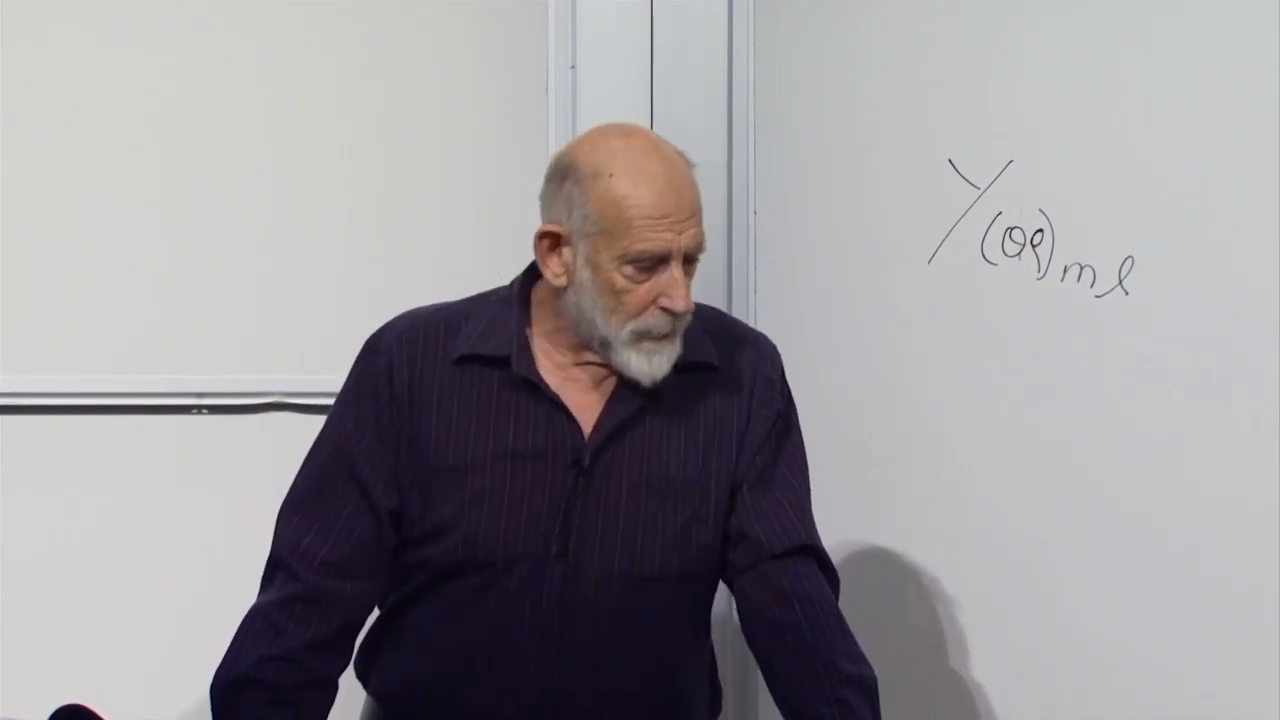
\includegraphics[width=0.9\linewidth]{lecture_03_frame_02.png}
\caption{При фиксированном классическом угловом моменте радиальный гамильтониан содержит радиальную кинетическую энергию, центробежный член \(L^2/(2mr^2)\) и центральный потенциал \(V(r)\).}
\lectureframe{00:47:15}
\end{figure}

Член \(1/r^2\) — это центробежный барьер. Он возрастает по мере приближения частицы к началу координат, поэтому соответствующая сила направлена наружу. Для обсуждаемых кулоноподобных притяжений траектория при \(L\neq0\) огибает центр вместо того, чтобы достигнуть его. При \(L=0\) барьер отсутствует.

Для притягательного кулоновского потенциала,
\begin{equation}
V(r)=-\frac{\kappa}{r},
\end{equation}
центробежный член доминирует при малых \(r\), тогда как кулоновский член убывает медленнее и доминирует при больших \(r\). При \(L\neq0\) их сумма имеет минимум. Движение в минимуме имеет постоянный радиус и потому является круговым. Связанное движение выше минимума и ниже порога убегания колеблется между наименьшим и наибольшим радиусами; в кулоновской задаче это радиальные колебания эллиптической орбиты.

\section{Редуцированное радиальное уравнение}

В квантовой механике угловая часть состояния с определённым орбитальным угловым моментом представляет собой сферическую гармонику. Запишем разделённое состояние как
\begin{equation}
\Psi_{n_r\ell m}(r,\theta,\phi)
=\frac{u_{n_r\ell}(r)}{r}\,
Y_{\ell m}(\theta,\phi).
\end{equation}
Угловой оператор \(L^2\) имеет собственное значение
\begin{equation}
L^2Y_{\ell m}
=\hbar^2\ell(\ell+1)Y_{\ell m}.
\end{equation}
Для фиксированной пары \(n_r,\ell\) будем сокращённо обозначать \(u_{n_r\ell}(r)\) через \(u(r)\). Уравнение, остающееся для редуцированной радиальной функции, имеет вид
\begin{equation}
\begin{aligned}
&-\frac{\hbar^2}{2m}\frac{d^2u}{dr^2}
+\frac{\hbar^2\ell(\ell+1)}{2mr^2}u(r)\\
&\qquad+V(r)u(r)=E_{n_r\ell}\,u(r).
\end{aligned}
\end{equation}

\editorialnote{Чисто одномерное уравнение со второй производной использует редуцированную радиальную функцию \(u=rR\). Поэтому \(\psi(r)\) в выписанном на лекции уравнении соответствует \(u(r)\), тогда как обычный радиальный множитель в \(\Psi=R(r)Y_{\ell m}\) есть \(R=u/r\). Это соглашение позволяет не рассматривать \(-i\hbar\,d/dr\) как самостоятельный эрмитов оператор радиального импульса в трёхмерном радиальном гильбертовом пространстве.}

Ниже на доске показано редуцированное радиальное уравнение.\footnote{Исходный кадр: \texttt{\detokenize{lecture_03_frame_03.png}}, видео лекции на отметке \(00{:}54{:}32\).}

\begin{figure}[htbp]
\centering
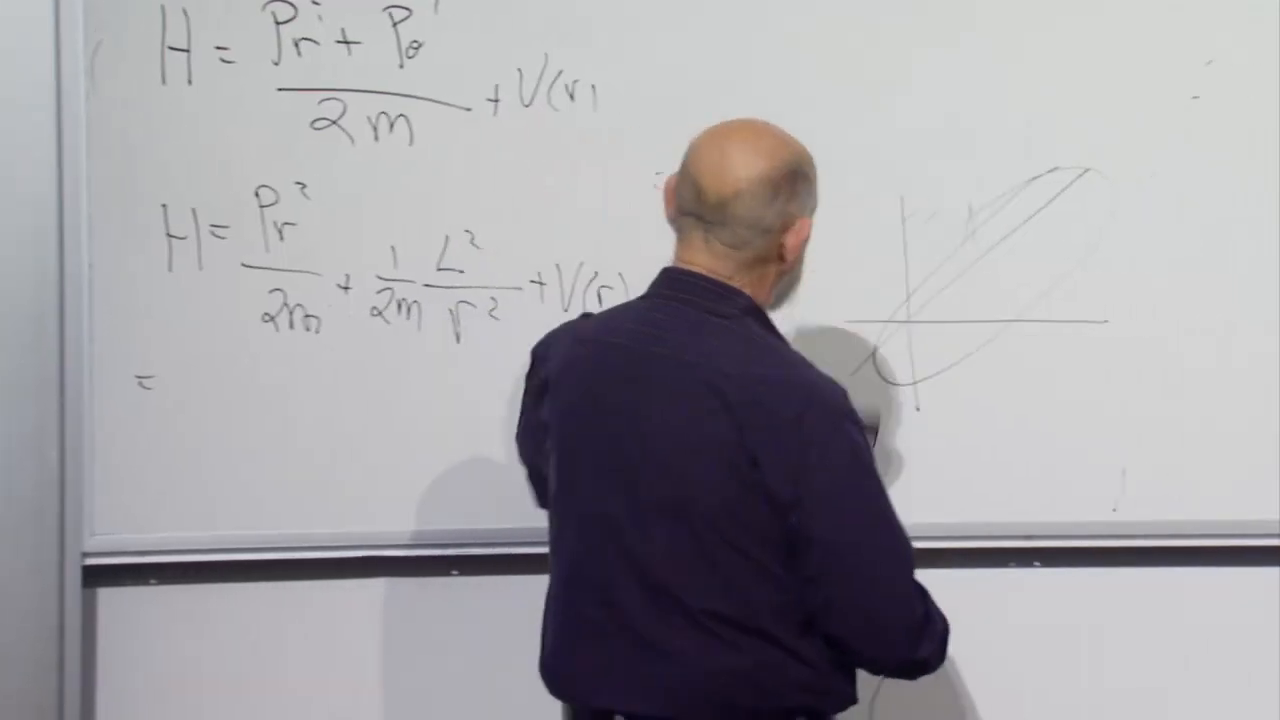
\includegraphics[width=0.9\linewidth]{lecture_03_frame_03.png}
\caption{При фиксированном \(\ell\) редуцированная радиальная волновая функция удовлетворяет одномерному уравнению Schr\"odinger с центробежным членом, пропорциональным \(\ell(\ell+1)/r^2\).}
\lectureframe{00:54:32}
\end{figure}

Трёхмерная угловая структура сведена к параметру \(\ell\). Магнитное квантовое число \(m\) не входит в радиальное уравнение.

\begin{classroomqa}
\lecturetimestamp{00:55:34}
\audiencequestion{Для данного \(\ell\) все ли \(2\ell+1\) магнитных состояний имеют одинаковую энергию?}
\lecturerresponse{Да, при условии, что радиальное собственное состояние тоже фиксировано. Для каждого выбранного \(u_{n_r\ell}\) все значения \(m=-\ell,\ldots,\ell\) имеют одинаковую энергию, потому что \(m\) не входит в радиальное уравнение. Разные радиальные собственные состояния при одном и том же \(\ell\), вообще говоря, имеют разные энергии.}
\end{classroomqa}

\begin{classroomqa}
\lecturetimestamp{00:56:03}
\audiencequestion{Почему \(L^2\) можно заменить на \(\hbar^2\ell(\ell+1)\), и как \(\ell\) связано с допустимыми значениями \(m\)?}
\lecturerresponse{Число \(\ell\) обозначает мультиплет углового момента и равно его наибольшему значению \(m\). Каждое состояние в этом мультиплете имеет одно и то же собственное значение \(L^2\), \(\hbar^2\ell(\ell+1)\), поэтому именно это собственное значение подставляется в радиальное уравнение.}
\end{classroomqa}

Явные решения через специальные функции для данного рассуждения не нужны. Важно то, как организованы решения.

\section{Радиальные узлы и энергетические уровни}

При фиксированном \(\ell\) приведённое радиальное уравнение представляет собой обычную одномерную задачу на собственные значения. Его связанные состояния упорядочены по числу внутренних узлов. Низшее радиальное состояние не имеет внутренних узлов, следующее имеет один, а следующее — два. Большее число узлов означает более быстрое изменение волновой функции; более быстрое изменение означает больший импульс и, следовательно, большую кинетическую энергию.

Каждое значение \(\ell\) задаёт свой радиальный оператор, поскольку центробежный член меняется с \(\ell\). Поэтому \(\ell=0,1,2,\ldots\) образуют отдельные радиальные башни. Положительный центробежный член сдвигает уровни вверх по мере увеличения углового момента. Каждому радиальному собственному значению при фиксированном \(\ell\) соответствует магнитный мультиплет размерности
\begin{equation}
2\ell+1.
\end{equation}
Уровни \(\ell=0\) — синглеты, уровни \(\ell=1\) — триплеты, а уровни \(\ell=2\) — квинтуплеты. Эти вырождения гарантируются вращательной симметрией; дополнительная симметрия может также сделать вырожденными состояния с разными значениями \(\ell\).

Для потенциалов атомного типа, удовлетворяющих \(V(r)\to0\) при больших \(r\), порог ухода по соглашению равен \(E=0\). Состояния с отрицательной энергией образуют дискретный связанный спектр. При \(E=0\) и выше встречается континуум рассеяния. Это утверждение зависит от поведения потенциала при больших \(r\) и не применимо к удерживающему центральному потенциалу.

\section{Особое кулоновское вырождение}

Точный нерелятивистский кулоновский потенциал обладает дополнительным совпадением уровней. Низшее радиальное состояние при \(\ell=1\) имеет ту же энергию, что и первое возбуждённое состояние при \(\ell=0\). Следующее состояние при \(\ell=1\) совпадает со вторым возбуждённым состоянием при \(\ell=0\), и к ним присоединяется низшее состояние при \(\ell=2\). Эта картина продолжается и в более высоких радиальных башнях и башнях углового момента.

\begin{classroomqa}
\lecturetimestamp{01:09:57}
\audiencequestion{Указывает ли это дополнительное кулоновское вырождение на ещё одну симметрию?}
\lecturerresponse{Да. Это необычная дополнительная симметрия точного кулоновского потенциала. Небольшие изменения потенциала разрушают это совпадение, и его вывод здесь не рассматривается.}
\end{classroomqa}

Соответствующие вырождения орбитальных оболочек таковы:
\begin{equation}
1,\qquad 4,\qquad 9,\qquad 16,\qquad \ldots
\end{equation}
до учёта электронного спина.

\begin{classroomqa}
\lecturetimestamp{01:11:46}
\audiencequestion{Описывает ли это вырождение водород или только идеальную кулоновскую задачу?}
\lecturerresponse{Для водорода оно выполняется с очень хорошей точностью, но не точно. Релятивистские поправки и конечный размер ядра нарушают идеальную кулоновскую картину.}
\end{classroomqa}

Точечное ядро создаёт точный потенциал \(1/r\). Ядро, заряд которого распределён по небольшому объёму, создаёт слегка иной потенциал, когда электрон проникает в этот объём, и даже это малое отклонение снимает часть особого вырождения.

Спин также был опущен. Учёт двух спиновых состояний электрона удваивает числа состояний в оболочках до
\begin{equation}
2,\qquad 8,\qquad 18,\qquad 32,\qquad \ldots
\end{equation}
прежде чем в более полном атомном рассмотрении будут разрешены дальнейшие расщепления.

\section{Возвращение к декартовому уравнению}

Уравнение, с которого началась радиальная задача, — это трёхмерное
стационарное уравнение Schr\"odinger
\begin{equation}
\begin{aligned}
-\frac{\hbar^2}{2m}\nabla^2\Psi+V(r)\Psi&=E\Psi,\\
\nabla^2&=\frac{\partial^2}{\partial x^2}
+\frac{\partial^2}{\partial y^2}
+\frac{\partial^2}{\partial z^2},\\
r&=\sqrt{x^2+y^2+z^2}.
\end{aligned}
\end{equation}
Перейдём к радиальным и угловым координатам и выберем собственное состояние \(L^2\).
Замена \(L^2\) на \(\hbar^2\ell(\ell+1)\) затем сводит это уравнение в частных
производных к обычному радиальному уравнению выше.

\begin{classroomqa}
\lecturetimestamp{01:16:42}
\audiencequestion{Можно ли использовать отклонения от идеального кулоновского спектра для определения размера ядра?}
\lecturerresponse{Не с помощью такого простого сравнения. Другие поправки намного больше, и их сначала нужно учесть. Размер ядра здесь упомянут потому, что он даёт наглядный пример отклонения от потенциала точечного Кулона.}
\end{classroomqa}

\begin{classroomqa}
\lecturetimestamp{01:17:09}
\audiencequestion{В чём главное отличие между классическим и квантовым членами углового момента?}
\lecturerresponse{Классически \(L^2\) — это обычный квадрат модуля сохраняющегося вектора. В квантовом орбитальном мультиплете его собственное значение равно \(\hbar^2\ell(\ell+1)\), а не просто \(\hbar^2\ell^2\). Дополнительный член возникает из-за некоммутативности компонент углового момента.}
\end{classroomqa}

\begin{classroomqa}
\lecturetimestamp{01:17:58}
\audiencequestion{Имеют ли волновые функции связанных состояний компактный носитель?}
\lecturerresponse{Нет. Они простираются сколь угодно далеко от центра. Для обсуждаемых атомных связанных состояний они убывают на больших расстояниях экспоненциально, так что вероятность становится пренебрежимо малой, но не обращается в нуль за пределами какого бы то ни было конечного радиуса.}
\end{classroomqa}

\begin{classroomqa}
\lecturetimestamp{01:18:48}
\audiencequestion{Когда \(\ell=0\) устраняет центробежную яму, что происходит с устойчивой точкой?}
\lecturerresponse{Минимум, возникающий из-за конкуренции между центробежным барьером и притяжением, исчезает. В идеализации точечного Кулона классическое движение направляется к сингулярному центру. Квантовомеханически низшее состояние не может иметь одновременно и точно определённое положение в центре, и нулевой импульс, так что низшая волновая функция имеет конечную пространственную протяжённость.}
\end{classroomqa}

\editorialnote{Для регулярного центрального потенциала классическая траектория с нулевым угловым моментом может проходить через начало координат. Для идеального точечно-кулоновского потенциала, напротив, \(r=0\) является сингулярностью столкновения, и продолжение классической траектории требует дополнительного предписания.}

В классической редукции одну орбиту поместили в плоскость, но тот же шаг нельзя таким же образом применить к квантовой волновой функции. Квантовое орбитальное состояние заполняет трёхмерное пространство. Полный угловой оператор имеет вид \(L^2=L_x^2+L_y^2+L_z^2\), и его собственное значение сохраняет трёхмерный результат \(\hbar^2\ell(\ell+1)\).

\begin{classroomqa}
\lecturetimestamp{01:21:30}
\audiencequestion{Как квантовая задача может оставаться трёхмерной после того, как классическую орбиту поместили в плоскость?}
\lecturerresponse{Лишь классическую орбиту поместили в фиксированную плоскость, выбрав систему координат так, чтобы эта плоскость была перпендикулярна сохраняющемуся вектору углового момента. Квантовая волновая функция занимает трёхмерное пространство. Другие компоненты углового момента по-прежнему присутствуют через \(L^2\), поэтому радиальное уравнение содержит \(\ell(\ell+1)\), а не только квадрат одной компоненты.}
\end{classroomqa}

\begin{classroomqa}
\lecturetimestamp{01:22:54}
\audiencequestion{Допускает ли всякая квантовая задача операторы повышения и понижения?}
\lecturerresponse{Нет. Они возникают в необычно благоприятных случаях. Угловой момент — один из них, а гармонический осциллятор — другой. Случай осциллятора особенно полезен, потому что движение вблизи устойчивого равновесия столь часто бывает приближённо гармоническим, включая малые радиальные колебания около минимума эффективного потенциала.}
\end{classroomqa}

На этом атомная задача откладывается в сторону, и следующим примером спектра, определяемого лестничными операторами, становится гармонический осциллятор.

\section{Малые колебания и гармонический осциллятор}

Вблизи устойчивого равновесия достаточно малое смещение часто приводит к гармоническому движению. Эффективный радиальный потенциал при ненулевом угловом моменте даёт один такой пример: радиальное движение вблизи дна его ямы приблизительно гармонично.

Рассмотрим одномерный осциллятор единичной массы. Пусть \(x\) — смещение от положения равновесия, а жёсткость пружины запишем как \(k=\omega^2\). Классический гамильтониан имеет вид
\begin{equation}
H=\frac{p^2}{2}+\frac{\omega^2x^2}{2}.
\end{equation}
Уравнения Гамильтона дают
\begin{equation}
\dot{x}=\frac{\partial H}{\partial p}=p,
\qquad
\dot{p}=-\frac{\partial H}{\partial x}=-\omega^2x,
\end{equation}
и, следовательно,
\begin{equation}
\ddot{x}=-\omega^2x.
\end{equation}
Таким образом, \(\omega\) — это классическая частота колебаний.

\section{Факторизация и энергия нулевой точки}

Квантовомеханически,
\begin{equation}
[x,p]=i\hbar.
\end{equation}
Гамильтониан есть сумма квадратов, что подсказывает факторизацию
\begin{align}
\frac{1}{2}(p+i\omega x)(p-i\omega x)
&=\frac{1}{2}\left(p^2+\omega^2x^2+i\omega[x,p]\right) \\
&=\frac{1}{2}\left(p^2+\omega^2x^2-\hbar\omega\right).
\end{align}
Отсюда
\begin{equation}
H=\frac{1}{2}(p+i\omega x)(p-i\omega x)
+\frac{1}{2}\hbar\omega.
\end{equation}
Аддитивный член \(\hbar\omega/2\) есть энергия нулевой точки.

Классически наименьшая энергия достигалась бы при \(x=p=0\). Квантовомеханически ни одно состояние не может иметь одновременно и положение, и импульс, точно фиксированные на нуле. Кроме того, два члена \(p^2/2\) и \(\omega^2x^2/2\) положительны и не могут компенсировать друг друга. Поэтому ненулевая энергия основного состояния неизбежна.

При вычислении с лестничными операторами общую аддитивную константу можно временно отложить и восстановить в конце.

\begin{classroomqa}
\lecturetimestamp{01:36:10}
\audiencequestion{Говорит ли положительный знак члена нулевой точки ещё о чём-нибудь?}
\lecturerresponse{Гамильтониан осциллятора — положительный оператор: это сумма положительных квадратов, так что его энергия не может быть отрицательной.}
\end{classroomqa}

\section{Лестница осциллятора}

Введём безразмерные операторы\footnote{Около \(01{:}37\)--\(01{:}42\) в вычислении используется \(\hbar=1\). В эти нормированные определения возвращён множитель \(\hbar\), так что \(A_\pm\) безразмерны, а их коммутатор равен единице.}
\begin{equation}
A_+=\frac{p+i\omega x}{\sqrt{2\hbar\omega}},
\qquad
A_-=\frac{p-i\omega x}{\sqrt{2\hbar\omega}}.
\end{equation}
Они эрмитово сопряжены друг другу:
\begin{equation}
A_+^\dagger=A_-.
\end{equation}
Их коммутатор равен
\begin{align}
[A_-,A_+]
&=\frac{1}{2\hbar\omega}
\left([p,i\omega x]+[-i\omega x,p]\right) \\
&=1.
\end{align}

Определим
\begin{equation}
N=A_+A_-.
\end{equation}
Тогда гамильтониан равен
\begin{equation}
H=\hbar\omega\left(N+\frac{1}{2}\right).
\end{equation}
Таким образом, нахождение энергетического спектра сводится к нахождению собственных значений \(N\).

Пусть
\begin{equation}
N|n\rangle=n|n\rangle.
\end{equation}
Коммутаторы с \(N\) имеют вид\footnote{Промежуточные шаги при \(01{:}45{:}37\)--\(01{:}48{:}10\) непосредственно восстанавливаются из приведённых соотношений \(N=A_+A_-\) и \([A_-,A_+]=1\).}
\begin{align}
[N,A_+]
&=A_+[A_-,A_+]=A_+, \\
[N,A_-]
&=[A_+,A_-]A_-=-A_-.
\end{align}
Отсюда следует, что
\begin{align}
N\bigl(A_+|n\rangle\bigr)
&=(n+1)A_+|n\rangle, \\
N\bigl(A_-|n\rangle\bigr)
&=(n-1)A_-|n\rangle.
\end{align}
Следовательно, \(A_+\) повышает собственное значение \(N\) на единицу, а \(A_-\) понижает его на единицу всякий раз, когда получающийся вектор не равен нулю.

Оператор \(N\) неотрицателен:
\begin{equation}
\langle\psi|N|\psi\rangle
=\langle\psi|A_+A_-|\psi\rangle
=\|A_-|\psi\rangle\|^2
\geq0.
\end{equation}
Поэтому процесс понижения не может продолжаться в область отрицательных собственных значений. На нижнем состоянии \(|b\rangle\) он должен прекратиться:
\begin{equation}
A_-|b\rangle=0.
\end{equation}

Для нормированных собственных состояний коэффициенты в лестничных соотношениях определяются их нормами:
\begin{align}
\|A_-|n\rangle\|^2
&=\langle n|A_+A_-|n\rangle=n, \\
\|A_+|n\rangle\|^2
&=\langle n|A_-A_+|n\rangle=n+1.
\end{align}
Поэтому фазы можно выбрать так, чтобы
\begin{equation}
A_-|n\rangle=\sqrt{n}\,|n-1\rangle,
\qquad
A_+|n\rangle=\sqrt{n+1}\,|n+1\rangle.
\end{equation}

\begin{classroomqa}
\lecturetimestamp{01:52:42}
\audiencequestion{Если \(A_-\) понижает состояние, а \(A_+\) поднимает его обратно, то как \(A_+A_-\) даёт собственное значение \(n\)?}
\lecturerresponse{В действие лестничных операторов входят нормировочные множители. Первое действие \(A_-\) даёт множитель \(\sqrt n\), а действие \(A_+\) на полученное состояние даёт ещё один множитель \(\sqrt n\). Их произведение равно \(n\).}
\end{classroomqa}

Действительно,
\begin{equation}
A_+A_-|n\rangle
=\sqrt n\,A_+|n-1\rangle
=n|n\rangle.
\end{equation}

\begin{classroomqa}
\lecturetimestamp{01:55:52}
\audiencequestion{Должно ли наименьшее собственное значение \(N\) быть нулём, или оно может быть положительным?}
\lecturerresponse{Оно должно быть нулём, и спектр \(N\) состоит из неотрицательных целых чисел. Доказательство того, где находится нижний конец спектра, пока ещё не приведено.}
\end{classroomqa}

\editorialnote{Пусть \(|b\rangle\) — нижнее состояние. Поскольку понижение должно прекратиться, \(A_-|b\rangle=0\). Отсюда немедленно следует, что \(N|b\rangle=A_+A_-|b\rangle=0\), так что наименьшее собственное значение \(N\) равно нулю.}

Начиная с этого нижнего состояния и применяя \(A_+\), получаем
\begin{equation}
n=0,1,2,\ldots.
\end{equation}
Восстанавливая аддитивный член нулевой энергии, получаем энергии осциллятора
\begin{equation}
E_n=\hbar\omega\left(n+\frac{1}{2}\right),
\qquad n=0,1,2,\ldots.
\end{equation}

Алгебра осциллятора будет в дальнейшем развита и использована для решения других квантовых задач.
\chapter{Волновые функции осциллятора, спин 1/2 и перестановка частиц}

\section{Осцилляторы повсюду}

Любая система с устойчивым равновесием может колебаться, если ее вывести из этого равновесия. У нее может быть одна частота или много. У струны скрипки, например, есть основная мода и высшие гармоники. Если ее щипнуть, возбуждается некоторая комбинация этих мод.

Более важные для нас примеры здесь — поля. Равновесная конфигурация электромагнитного поля — это вакуум: нет ни электрического поля, ни магнитного поля, ни электромагнитных колебаний. Если ввести излучение в полость или волновод, поле может колебаться в своих разрешенных модах, каждая со своей собственной частотой. В квантовой теории эти моды описывают совокупности фотонов.

Та же идея применима к кристаллу. Представлять каждый атом как независимый осциллятор вводит в заблуждение. Атомы действуют друг на друга силами, так что смещение одного атома влияет на его соседей, и через кристалл проходит волна. Нормальные моды этого связанного движения являются гармоническими осцилляторами, а их кванты называются фононами. Фотоны и фононы — разные физические объекты, но и те и другие приводят к одной и той же алгебре осциллятора.

\section{Алгебра осциллятора}

При обсуждении осциллятора положим массу и приведенную постоянную Планка равными 1:
\[
m=1,\qquad \hbar=1.
\]
Гамильтониан имеет вид
\begin{equation}
H=\frac{p^{2}}{2}+\frac{\omega^{2}x^{2}}{2}.
\end{equation}
Параметр \(\omega\) задает кривизну потенциала и одновременно является частотой колебаний.

Введем операторы повышения и понижения:
\begin{equation}
A_{\pm}=\frac{p\pm i\omega x}{\sqrt{2\omega}}.
\end{equation}
Нормировка выбрана так, что
\begin{equation}
[A_{-},A_{+}]=1.
\end{equation}
Оператор числа имеет вид
\begin{equation}
N=A_{+}A_{-}.
\end{equation}
Вместе эти уравнения означают, что \(A_{+}\) увеличивает собственное значение \(N\) на единицу, а \(A_{-}\) уменьшает его на единицу. Получающийся спектр таков:
\begin{equation}
n=0,1,2,3,\ldots .
\end{equation}

Произведение двух лестничных операторов также выявляет квантовую поправку к классической энергии:
\begin{align}
N
&=\frac{1}{2\omega}(p+i\omega x)(p-i\omega x)\\
&=\frac{1}{2\omega}\left(p^{2}+\omega^{2}x^{2}
 +i\omega[x,p]\right)\\
&=\frac{1}{2\omega}\left(p^{2}+\omega^{2}x^{2}-\omega\right),
\end{align}
где \([x,p]=i\). Следовательно,
\begin{equation}
H=\omega\left(N+\frac12\right).
\end{equation}
Если аддитивная константа для задачи несущественна, удобно использовать сдвинутый гамильтониан
\begin{equation}
H_{\mathrm{shifted}}=H-\frac{\omega}{2}=\omega N.
\end{equation}
Член \(\omega/2\) — это энергия нулевых колебаний осциллятора, то есть энергия основного состояния. Для моды поля аналогичный член называется энергией вакуума. Он отражает принцип неопределенности: ни одно состояние не может иметь одновременно \(x\) и \(p\), точно равные нулю, так что два положительных квадратичных члена в \(H\) не могут оба иметь нулевое среднее значение.

\begin{classroomqa}
\lecturetimestamp{00:09:46}
\audiencequestion{Почему нуль входит в спектр оператора числа?}
\lecturerresponse{Это можно явно показать, построив волновую функцию основного состояния. Это построение выявит состояние с \(N=0\).}
\end{classroomqa}

Чтобы начать это построение, заменим векторы состояния волновыми функциями координаты. Собственные состояния энергии принимают вид
\[
\psi_{0}(x),\ \psi_{1}(x),\ \psi_{2}(x),\ldots,
\]
а основные операторы действуют как
\begin{equation}
X\longmapsto x,\qquad
P\longmapsto -i\frac{d}{dx}.
\end{equation}
Если восстановить \(\hbar\), вторая замена примет вид
\(P\mapsto-i\hbar\,d/dx\).

Прежде чем решать для \(\psi_{0}\), на этот вопрос есть более быстрый абстрактный ответ. На дискретной лестнице нормируемых собственных состояний осциллятора \(N=A_{+}A_{-}\) неотрицателен, поэтому многократное понижение шагами по единице не может продолжаться бесконечно. В нижнем конце---чью нормируемую волновую функцию мы построим ниже---должно существовать состояние, обозначаемое \(\lvert0\rangle\), для которого
\begin{equation}
A_{-}\lvert0\rangle=\mathbf 0.
\end{equation}
Иначе \(A_{-}\lvert0\rangle\) было бы еще одним состоянием на одну ступень ниже. Отсюда сразу следует, что
\begin{equation}
N\lvert0\rangle
=A_{+}A_{-}\lvert0\rangle
=\mathbf 0
=0\,\lvert0\rangle.
\end{equation}
Таким образом, нижнее состояние имеет нулевое собственное значение оператора числа.

\begin{classroomqa}
\lecturetimestamp{00:14:57}
\audiencequestion{Если собственное значение равно нулю, не должен ли правый член содержать нулевой собственный вектор?}
\lecturerresponse{Кет \(\lvert0\rangle\) — это нормированный ненулевой вектор с меткой нуль. В \(N\lvert0\rangle=0\,\lvert0\rangle\) правая часть — нулевой вектор. Кет основного состояния и нулевой вектор — разные объекты.}
\end{classroomqa}

\section{Уравнение Schr\"odinger и физические решения}

Теперь вернемся к координатному представлению. Стационарное уравнение Schr\"odinger имеет вид
\begin{equation}
\left[
-\frac12\frac{d^{2}}{dx^{2}}
+\frac12\omega^{2}x^{2}
\right]\psi(x)=E\psi(x).
\end{equation}
Как дифференциальное уравнение второго порядка, оно имеет формальные решения при произвольных значениях \(E\). Большинство этих формальных решений не являются физическими состояниями осциллятора. При больших \(\lvert x\rvert\) они растут экспоненциально, так что их норма расходится.

Для связанного состояния волновая функция должна быть квадратично интегрируемой:
\begin{equation}
\int_{-\infty}^{\infty}\psi^{*}(x)\psi(x)\,dx<\infty.
\end{equation}
Тогда ее можно нормировать так, чтобы интеграл был равен единице. Только специальные значения энергии дают такие решения. Координатные и импульсные состояния на бесконечной прямой в этом отношении составляют исключение, но экспоненциально растущие решения осциллятора просто исключаются из пространства состояний.

\section{Гауссово основное состояние}

Уравнение второго порядка можно решить, но алгебра лестничных операторов дает более простое уравнение первого порядка:
\begin{equation}
A_{-}\psi_{0}(x)=0.
\end{equation}
Общий множитель в \(A_{-}\) несущественен, когда правая часть равна нулю, поэтому это равносильно
\begin{equation}
(p-i\omega x)\psi_{0}(x)=0.
\end{equation}
Используя \(p=-i\,d/dx\), получаем
\begin{equation}
\left(\frac{d}{dx}+\omega x\right)\psi_{0}(x)=0.
\end{equation}

\begin{classroomqa}
\lecturetimestamp{00:22:32}
\audiencequestion{Можно ли было бы решить это разделением переменных?}
\lecturerresponse{Здесь есть только одна независимая переменная, так что двух переменных для разделения нет. В записи \(\psi_{0}'/\psi_{0}=-\omega x\) это уравнение имеет вид логарифмической производной. Это подсказывает записать волновую функцию в экспоненциальной форме.}
\end{classroomqa}

Удобно искать решение в виде
\begin{equation}
\psi_{0}(x)=e^{f(x)}.
\end{equation}
Тогда
\[
\psi_{0}'(x)=f'(x)e^{f(x)},
\]
и общий экспоненциальный множитель сокращается. Уравнение сводится к
\begin{equation}
\frac{df}{dx}+\omega x=0.
\end{equation}

\begin{classroomqa}
\lecturetimestamp{00:26:28}
\audiencequestion{Не должен ли в \(f(x)\) стоять знак минус?}
\lecturerresponse{Да. Поскольку \(df/dx=-\omega x\), интегрирование дает отрицательный квадратичный член.}
\end{classroomqa}

Следовательно,
\begin{equation}
f(x)=-\frac12\omega x^{2}+C,
\end{equation}
и
\begin{equation}
\psi_{0}(x)\propto e^{-\omega x^{2}/2}.
\end{equation}
Мультипликативная нормировочная константа оставлена неопределенной. Важна гауссова форма: функция гладкая, сосредоточена вблизи начала координат и быстро убывает при больших \(\lvert x\rvert\). Она очевидным образом квадратично интегрируема.

Нет необходимости подставлять ответ обратно в уравнение второго порядка, чтобы узнать его энергию. Алгебра уже дает
\begin{equation}
E_{0}=\frac{\omega}{2}.
\end{equation}

\section{Возбужденные состояния, узлы и классическое движение}

Первое возбужденное состояние получается действием оператора повышения на основное состояние:
\begin{equation}
\psi_{1}(x)\propto A_{+}\psi_{0}(x)
\propto(p+i\omega x)e^{-\omega x^{2}/2}.
\end{equation}
Из уравнения для основного состояния следует
\[
p\psi_{0}=i\omega x\,\psi_{0}.
\]
Смена знака в лестничном операторе превращает сокращение в сложение:
\begin{equation}
(p+i\omega x)\psi_{0}
=2i\omega x\,\psi_{0}.
\end{equation}
С точностью до общего множителя,
\begin{equation}
\psi_{1}(x)\propto x\,e^{-\omega x^{2}/2}.
\end{equation}

Эта волновая функция нечетна:
\begin{equation}
\psi_{1}(-x)=-\psi_{1}(x).
\end{equation}
Ее плотность вероятности четна, но в начале координат у нее есть узел,
\begin{equation}
\lvert\psi_{1}(0)\rvert^{2}=0.
\end{equation}
Следовательно, плотность вероятности первого возбужденного состояния имеет узел при \(x=0\).

Многократное действие \(A_{+}\) дает многочлены все более высокой степени, умножающие ту же гауссову оболочку.\footnote{В лекции указаны многочленные множители более высокой степени, дополнительный узел на каждом шаге и чередование четности в промежутке от \(00{:}34{:}25\) до \(00{:}35{:}49\). Вид произведения гауссиана на многочлен подтверждается также в книге Leonard Susskind и Art Friedman, \emph{Quantum Mechanics: The Theoretical Minimum} (2014), при обсуждении собственных функций осциллятора.} С точностью до нормировки,
\begin{equation}
\psi_{n}(x)=P_{n}(x)e^{-\omega x^{2}/2}.
\end{equation}
Четность чередуется между четной и нечетной, и каждый шаг добавляет узел. С ростом \(n\) волновая функция простирается дальше от начала координат и приобретает более быстрые осцилляции.

Эти две особенности имеют прямой физический смысл. То, что волновая функция заметна дальше от начала координат, соответствует большей потенциальной энергии, потому что потенциал растет как \(x^{2}\). Быстрые осцилляции в координатном пространстве указывают на больший импульс. Сильно возбужденный осциллятор с большей вероятностью удаляется дальше от центра; когда он проходит через центральную область, он несет больший импульс, и там его волновая функция осциллирует быстрее.

\begin{classroomqa}
\lecturetimestamp{00:37:18}
\audiencequestion{Разве гармонический осциллятор не приближается к классическому поведению, когда \(n\) становится большим?}
\lecturerresponse{Классическое движение не представляется одним стационарным собственным состоянием энергии. Оно возникает в волновом пакете, содержащем много энергетических уровней. Сдвинутый гауссиан, например, эволюционирует туда и обратно как классический осциллятор, а относительная неопределенность становится меньше по мере того, как размах колебаний растет.}
\end{classroomqa}

Возьмем гауссиан основного состояния и сместим его от начала координат. Сдвинутый пакет больше не является собственным состоянием энергии; он представляет собой суперпозицию многих таких состояний. Согласно зависящему от времени уравнению Schr\"odinger его компоненты приобретают разные фазы. Пакет колеблется от одной стороны потенциала к другой, приобретая быстрые изменения фазы вблизи центра и снова становясь гладким вблизи точки поворота. Чем больше размах по сравнению с шириной пакета, тем ближе движение к классическому.

\begin{classroomqa}
\lecturetimestamp{00:39:29}
\audiencequestion{Должна ли волновая функция второго возбужденного состояния проходить через нуль в начале координат?}
\lecturerresponse{Нет. Ее многочленный множитель — не просто \(x^{2}\); он также содержит постоянный член, так что волновая функция не обязана обращаться в нуль при \(x=0\).}
\end{classroomqa}

Аргумент с лестничными операторами также предполагает, что \(A_{+}\) и \(A_{-}\) являются эрмитово-сопряжёнными друг другу на области определения осциллятора, состоящей из квадратично интегрируемых функций, с граничным поведением, необходимым для соотношения сопряжённости. Формальные решения, растущие экспоненциально, этой области не принадлежат.

\begin{classroomqa}
\lecturetimestamp{00:40:45}
\audiencequestion{Существует ли общий способ распознать, когда гамильтониан может быть решён этими алгебраическими методами?}
\lecturerresponse{Такого общего правила нет. Точно решаемые примеры редки. Гармонический осциллятор и идеальный нерелятивистский атом водорода — удачные случаи, в которых алгебраические методы работают.}
\end{classroomqa}

\section{Спин 1/2 как момент импульса}

Спин — это момент импульса, которым частица обладает независимо от орбитального движения своего центра масс. Покоящаяся частица не имеет орбитального момента импульса \(\mathbf R\times\mathbf P\), но всё же может иметь спин. Можно пытаться представить себе крошечный вращающийся объект или рассматривать спин как внутреннее квантовое свойство. Решающим является математическое утверждение: его компоненты преобразуются при пространственных вращениях и удовлетворяют коммутационным соотношениям для момента импульса.

Начиная с этого места, снова восстановим \(\hbar\). Компоненты момента импульса удовлетворяют
\begin{equation}
[L_{z},L_{x}]=i\hbar L_{y},
\end{equation}
а два других соотношения получаются циклической перестановкой. Безразмерные матрицы Паули имеют вид
\begin{equation}
\begin{aligned}
\sigma_{z}&=
\begin{pmatrix}
1&0\\
0&-1
\end{pmatrix},\\[0.4em]
\sigma_{x}&=
\begin{pmatrix}
0&1\\
1&0
\end{pmatrix},\\[0.4em]
\sigma_{y}&=
\begin{pmatrix}
0&-i\\
i&0
\end{pmatrix}.
\end{aligned}
\end{equation}
В этом базисе \(\sigma_{z}\) диагональна. Её собственные значения равны \(+1\) и
\(-1\).

\begin{classroomqa}
\lecturetimestamp{00:47:35}
\audiencequestion{Есть ли знак минус в \(\sigma_x\)?}
\lecturerresponse{Нет. Оба внедиагональных элемента \(\sigma_x\) положительны.}
\end{classroomqa}

Вычисление на доске в \(00{:}49{:}35\) начинает покомпонентное
умножение матриц. Доведение произведений до конца даёт
\begin{align}
\sigma_{z}\sigma_{x}
&=
\begin{pmatrix}
0&1\\
-1&0
\end{pmatrix}
=i\sigma_{y},\\
\sigma_{x}\sigma_{z}
&=
\begin{pmatrix}
0&-1\\
1&0
\end{pmatrix}
=-i\sigma_{y}.
\end{align}
Следовательно,
\begin{equation}
[\sigma_{z},\sigma_{x}]=2i\sigma_{y}.
\end{equation}
Лишний множитель 2 устраняется, если определить физические операторы спина как\footnote{Вычисление на доске опускает \(\hbar\). Здесь он восстановлен, так что \(S_i\) имеет размерность момента импульса.}
\begin{equation}
S_{i}=\frac{\hbar}{2}\sigma_{i}.
\end{equation}
Тогда
\begin{equation}
[S_{z},S_{x}]=i\hbar S_{y},
\end{equation}
и аналогично для циклических перестановок. Следовательно, половины матриц Паули, с восстановленным множителем \(\hbar\), образуют систему момента импульса.

Положив \(\hbar=1\), получаем вид, показанный ниже.\footnote{Исходный кадр — \texttt{lecture\_04\_frame\_02.png}.}
\begin{figure}[htbp]
\centering
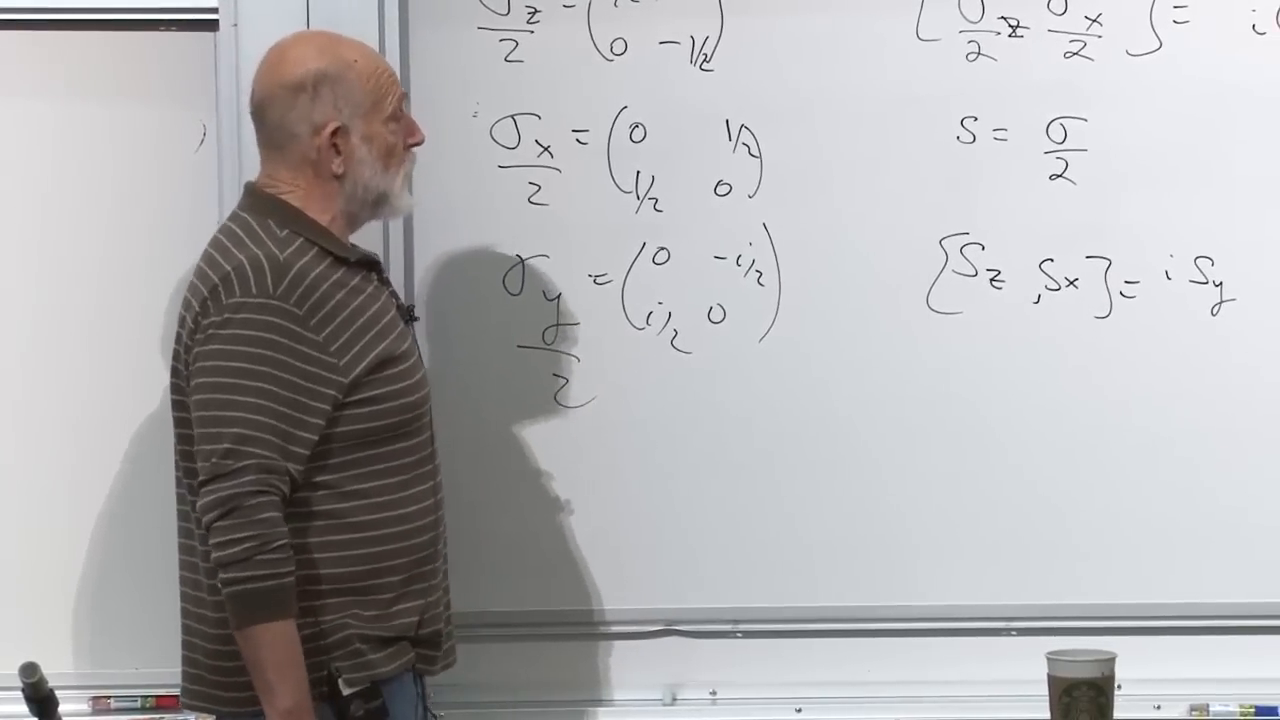
\includegraphics[width=0.9\linewidth]{lecture_04_frame_02.png}
\caption{В единицах, где \(\hbar=1\), половины матриц Паули являются операторами момента импульса для спина 1/2 и удовлетворяют соотношению \([S_z,S_x]=iS_y\).}
\lectureframe{00:55:41}
\end{figure}

Два уравнения на собственные значения для \(S_z\) имеют вид
\begin{equation}
S_z\lvert\pm\rangle
=\pm\frac{\hbar}{2}\lvert\pm\rangle.
\end{equation}
Эквивалентно, безразмерное магнитное квантовое число равно
\begin{equation}
m_{s}=\pm\frac12,
\qquad
S_{z}\lvert m_{s}\rangle
=m_{s}\hbar\,\lvert m_{s}\rangle.
\end{equation}
Операторы повышения и понижения момента импульса изменяют \(m\) целыми шагами, но это не требует, чтобы каждая лестница проходила через нуль. Целочисленные мультиплеты содержат целые значения \(m\), тогда как полуцелые мультиплеты содержат полуцелые значения. Для спина 1/2 лестница имеет только два члена \(m_s=+1/2\) и \(m_s=-1/2\).

Эти два состояния образуют дублет спина 1/2. К числу частиц, описываемых такими мультиплетами с полуцелым спином, относятся электроны, мюоны, нейтрино и кварки.

\section{Орбитальный и спиновый момент импульса}

Теперь имеются два вида момента импульса. Орбитальный момент импульса описывает движение относительно начала координат,
\begin{equation}
\mathbf L=\mathbf R\times\mathbf P,
\end{equation}
тогда как \(\mathbf S\) — внутренний спин. Их векторная сумма есть полный момент импульса,
\begin{equation}
\mathbf J=\mathbf L+\mathbf S.
\end{equation}

\begin{classroomqa}
\lecturetimestamp{00:56:49}
\audiencequestion{Если система имеет полный момент импульса \(\mathbf J\), как определить её спин \(\mathbf S\)?}
\lecturerresponse{Квантовые числа спина и орбитального момента обычно задаются отдельно. Если \(L=0\), весь момент импульса является спином. В противном случае нужны квантовые правила сложения моментов импульса, которые здесь пока откладываются.}
\end{classroomqa}

Правила сложения в равной мере применимы к сумме орбитального момента импульса и спина, к двум спинам или к двум орбитальным моментам импульса. Объединённая система имеет собственные допустимые значения полного момента импульса, но эти правила нам пока не нужны.

\begin{classroomqa}
\lecturetimestamp{00:58:18}
\audiencequestion{Какие экспериментальные данные привели к введению спина?}
\lecturerresponse{Свидетельства дала спектроскопия, но периодическая таблица даёт особенно наглядную мотивацию: её оболочечная структура требует, чтобы электроны обладали дополнительным двузначным свойством.}
\end{classroomqa}

\section{Водородоподобное вырождение и подсчёт оболочек}

Для орбитального момента импульса уравнение на собственные значения \(L^{2}\) имеет вид
\begin{equation}
L^{2}\lvert\ell,m\rangle
=\hbar^{2}\ell(\ell+1)\lvert\ell,m\rangle,
\end{equation}
и фиксированному значению \(\ell\) соответствуют
\begin{equation}
2\ell+1
\end{equation}
магнитных состояний, отвечающих \(m=-\ell,-\ell+1,\ldots,\ell\).

Идеальная нерелятивистская кулоновская задача имеет дополнительное вырождение. Энергии её связанных состояний отрицательны и стремятся к нулю снизу, но для подсчёта важно только выравнивание уровней. Первый уровень с \(\ell=1\) совпадает по энергии со следующим уровнем с \(\ell=0\); первый уровень с \(\ell=2\) присоединяется к следующей главной оболочке; и эта схема продолжается.\footnote{\texttt{lecture\_04\_frame\_03.png}, \(01{:}02{:}01\); полное выравнивание по главным оболочкам изложено с \(01{:}02{:}33\) по \(01{:}04{:}10\).}

\begin{figure}[htbp]
\centering
\begin{tikzpicture}[x=1.55cm,y=1.0cm]
\draw[->] (-0.65,0) -- (-0.65,4.35);
\draw[->] (-0.85,0) -- (4.75,0);
\node at (-0.95,4.08) {\(E\)};
\node at (4.55,-0.28) {\(\ell\)};
\node at (0,-0.30) {\(0\)};
\node at (2,-0.30) {\(1\)};
\node at (4,-0.30) {\(2\)};

\draw (-0.20,0.75) -- (0.20,0.75);

\draw (-0.20,2.00) -- (0.20,2.00);
\foreach \dx in {-0.18,0,0.18}
  \draw (2+\dx-0.06,2.00) -- (2+\dx+0.06,2.00);

\draw (-0.20,3.15) -- (0.20,3.15);
\foreach \dx in {-0.18,0,0.18}
  \draw (2+\dx-0.06,3.15) -- (2+\dx+0.06,3.15);
\foreach \dx in {-0.32,-0.16,0,0.16,0.32}
  \draw (4+\dx-0.05,3.15) -- (4+\dx+0.05,3.15);

\node[anchor=west] at (0.35,0.75) {\(n=1\)};
\node[anchor=west] at (2.35,2.00) {\(n=2\)};
\node[anchor=west] at (4.40,3.15) {\(n=3\)};
\end{tikzpicture}
\caption{Первые три идеальные кулоновские оболочки объединяют орбитальные мультиплеты с одинаковой главной энергией: одно состояние в первой оболочке, \(1+3\) во второй и \(1+3+5\) в третьей.}
\lectureframe{01:02:01}
\end{figure}

В главной оболочке \(n\) допустимые орбитальные квантовые числа таковы\footnote{Этот компактный диапазон \(\ell\) и приведённая ниже сумма воспроизводят выравнивание уровней и числа \(1,4,9,16,\ldots\), указанные с \(01{:}02{:}33\) по \(01{:}04{:}10\). Начало рисунка спектра показано в \texttt{lecture\_04\_frame\_03.png} при \(01{:}02{:}01\).}
\[
\ell=0,1,\ldots,n-1.
\]
Поэтому число пространственных состояний равно
\begin{equation}
\sum_{\ell=0}^{n-1}(2\ell+1)=n^{2},
\end{equation}
что даёт последовательность
\begin{equation}
1,\ 4,\ 9,\ 16,\ldots .
\end{equation}
Это только орбитальный подсчёт. Каждому пространственному состоянию соответствуют два значения спина, так что соответствующие идеализированные суммарные числа таковы
\begin{equation}
2,\ 8,\ 18,\ 32,\ldots=2n^{2}.
\end{equation}

\section{Принцип запрета и двузначное свойство электрона}

Начнём с гелия в приближении независимых электронов. Его ядро имеет заряд, вдвое больший протонного, что перескалирует водородоподобные уровни и стягивает электроны внутрь. Игнорируя пока электрон--электронные взаимодействия, два электрона могут занимать самую низкую пространственную орбиталь и давать разумное первое приближение к основному состоянию гелия.

Почему бы не поместить туда и третий электрон? Это понизило бы его орбитальную энергию, но так не происходит. Ограничение задаётся принципом запрета Паули: никакие два электрона не могут занимать одно и то же полное одночастичное состояние. Называть это обычной силой отталкивания было бы вводящим в заблуждение. Это ограничение на допустимое квантовое состояние.

Возникает кажущееся противоречие. Два электрона в гелии действительно занимают одну и ту же пространственную орбиталь. Разрешение состоит в том, что полное состояние электрона включает не только орбитальную волновую функцию. Оно также включает двузначную степень свободы. Назовём эти значения вверх и вниз. Один электрон на самой низкой орбитали может иметь спин вверх, а другой — спин вниз; их пространственные состояния совпадают, но полные квантовые состояния не совпадают.

На этом месте подсчёт сначала идёт вперёд к литию, а затем возвращается назад. Это возвращение показывает, почему необходимы и запрет, и спин. Представим себе правило запрета вообще без спина. Только один электрон мог бы занимать самое низкое пространственное состояние. Второй электрон должен был бы попасть в одно из четырёх пространственных состояний следующей главной оболочки, что дало бы несколько альтернатив там, где наблюдаемое основное состояние гелия единственно. Такая бесспиновая версия принципа запрета неверна.

Теперь восстановим два значения спина. Два электрона заполняют самую низкую орбиталь с противоположными спинами. Третий электрон, как в нейтральном литии, должен попасть в следующую главную оболочку. Эта оболочка имеет одно пространственное состояние \(\ell=0\) и три пространственных состояния \(\ell=1\). До учёта спина имеется четыре возможности.

\begin{classroomqa}
\lecturetimestamp{01:14:58}
\audiencequestion{Как состояния \(s\) и \(p\) дают 8 возможностей в первой возбуждённой оболочке?}
\lecturerresponse{Имеется одно пространственное состояние с \(\ell=0\) и три с \(\ell=1\), всего четыре пространственных состояния. Каждое допускает два значения спина, так что общее число равно \(2(1+3)=8\).}
\end{classroomqa}

Именно этот простой подсчёт лежит в основе восьми позиций во второй строке периодической таблицы. Это намеренная идеализация: из дальнейшего обсуждения станет ясно, что электрон--электронные взаимодействия вскоре нарушают картину независимых водородоподобных оболочек.

Это двузначное свойство можно также проверить, рассматривая его как угловой момент. Спин электрона сопровождается магнитным моментом, поэтому магнитное поле придаёт двум его спиновым проекциям разные энергии. Уровень, который был вырожден в отсутствие поля, расщепляется на два, как и следует ожидать для малого магнитного момента, направленного вдоль поля или против него. Это расщепление проверяет, ведёт ли добавленная двузначная степень свободы себя как угловой момент, а не как произвольная двоичная метка.

\section{Фотоны, электроны и пределы оболочечной модели}

Не все частицы подчиняются одному и тому же правилу заполнения состояний. Многие фотоны могут занимать одну и ту же электромагнитную моду; классическую световую волну можно понимать как состояние, содержащее большое число фотонов в этой моде. Электроны ведут себя иначе: принцип запрета не позволяет им скапливаться в одном и том же полном квантовом состоянии. Этот контраст и побуждает различать две статистики частиц.

\begin{classroomqa}
\lecturetimestamp{01:20:28}
\audiencequestion{Что происходит в случае свободного потока электронов, а не электронов, связанных в атомах?}
\lecturerresponse{Правило запрета по-прежнему действует: электроны не могут все занимать одно квантовое состояние. Лазер может поместить много фотонов в одну и ту же моду, но поток электронов нельзя подготовить таким образом.}
\end{classroomqa}

Это ограничение — свойство электронов, а не особенность связывания в атоме.

\begin{classroomqa}
\lecturetimestamp{01:21:12}
\audiencequestion{Орбитальный угловой момент — это именно вращение вокруг ядра?}
\lecturerresponse{Угловой момент определяется относительно выбранного начала отсчёта. В атоме естественным началом служит ядро, тогда как у свободной частицы относительно любого выбранного начала угловой момент равен \(\mathbf R\times\mathbf P\).}
\end{classroomqa}

Каждое обсуждение вращения предполагает выбор точки, относительно которой это вращение совершается. Атом задаёт естественный центр, потому что его ядро является центром приблизительно центрального потенциала. В свободном пространстве никакое начало не выделено, хотя угловой момент всё равно можно вычислить относительно любого выбранного начала.

\begin{classroomqa}
\lecturetimestamp{01:22:34}
\audiencequestion{Почему в периодической таблице повторяются сначала ряды по 8, а затем ряды по 18 элементов?}
\lecturerresponse{Простая оболочечная модель независимых электронов не объясняет полной картины. Она быстро перестаёт работать, потому что пренебрегает взаимодействиями между электронами.}
\end{classroomqa}

Для большого атома внешние электроны взаимодействуют со значительным внутренним электронным облаком, а также с ядром. Считать, что каждый электрон движется независимо в неэкранированном кулоновском поле, уже неразумно.

\begin{classroomqa}
\lecturetimestamp{01:23:33}
\audiencequestion{Почему атомы не становятся резко больше по мере добавления электронов?}
\lecturerresponse{Добавление электронов означает и добавление протонов в ядро. Возросший заряд ядра подтягивает внутренние электроны внутрь, а эти внутренние электроны экранируют ядро. В этой простой картине внешний валентный электрон тогда движется в поле эффективного заряда, примерно равного единице.}
\end{classroomqa}

Возросший ядерный заряд стягивает внутреннее облако. Для атома с одним внешним валентным электроном ядро и внутренние электроны на больших расстояниях почти компенсируют друг друга, оставляя валентный электрон в поле, приблизительно таком же, как поле единичного положительного заряда. Поэтому размеры атомов не растут просто пропорционально числу электронов.

\begin{classroomqa}
\lecturetimestamp{01:24:49}
\audiencequestion{Является ли электрическое отталкивание причиной того, что соседние атомы остаются разделёнными?}
\lecturerresponse{Само по себе — нет. Принцип запрета Паули даёт важное эффективное отталкивание при перекрытии электронных облаков, и для многих атомов именно оно является главной причиной того, что они сопротивляются дальнейшему перекрытию.}
\end{classroomqa}

Отталкивание Паули — это эффективное следствие запрета, а не отдельный закон взаимодействия.

\begin{classroomqa}
\lecturetimestamp{01:25:23}
\audiencequestion{Является ли принцип запрета отдельным постулатом?}
\lecturerresponse{В нерелятивистской квантовой механике он вводится как постулат. В релятивистской квантовой теории связь спин--статистика даёт ему более глубокое основание.}
\end{classroomqa}

\section{Тождественные частицы в классической и квантовой механике}

Прежде чем формулировать этот постулат, рассмотрим, как тождественные частицы подсчитываются в классической теории. Поместим две частицы одного и того же вида в набор ящиков. Если частицы втайне носят имена---Гарри и Салли---, то конфигурация, где Гарри в первом ящике, а Салли во втором, кажется отличной от конфигурации, где Салли в первом, а Гарри во втором.

Классическая механика допускает такую картину даже тогда, когда метки слишком слабы, чтобы их обнаружить. Можно вообразить на каждой частице сколь угодно слабую отметку и всё же считать их траектории различными. В классической статистической механике обычно предпочитают не считать перестановки тождественных частиц новыми конфигурациями. Для \(N\) частиц это соглашение даёт привычный множитель \(1/N!\).

Квантовая механика строже. Тождественные частицы не несут скрытых индивидуальных меток, которые в принципе можно было бы проследить. Два электрона взаимозаменяемы как электроны. Перестановка электрона с фотоном дала бы физически иное расположение, потому что это разные виды частиц, но перестановка двух электронных мест не может выявить, какой электрон в действительности был каким.

Одночастичному состоянию соответствует волновая функция
\[
\psi(x)=\langle x\vert\psi\rangle.
\]
Для двух частиц состояние является функцией двух координатных аргументов,
\begin{equation}
\psi(x_{1},x_{2}).
\end{equation}
Индексы обозначают два места в описании, а не два пространственных направления. Квадрат её модуля даёт совместную плотность вероятности положений.

\section{Оператор перестановки и постулат о статистике}

Поменяем местами два места, соответствующие частицам:
\begin{equation}
\psi(x_{1},x_{2})\longmapsto\psi(x_{2},x_{1}).
\end{equation}
Следуя обозначениям, используемым в этом обсуждении, обозначим оператор перестановки через \(S\). Здесь \(S\) обозначает обмен, а не вектор спина \(\mathbf S\). Он действует так:
\begin{equation}
(S\psi)(x_{1},x_{2})=\psi(x_{2},x_{1}).
\end{equation}
Произвольная функция двух переменных не обязана быть симметричной, так что эта операция может дать другую волновую функцию.

Двойная перестановка восстанавливает исходный порядок:
\begin{equation}
S^{2}=I.
\end{equation}
Перестановка обратима и сохраняет скалярные произведения, поэтому она представляется унитарным оператором. Если \(\psi\) — собственный вектор \(S\) с собственным значением \(\lambda\), то
\[
S^{2}\psi=\lambda^{2}\psi=\psi,
\]
и, следовательно,
\begin{equation}
\lambda=\pm1.
\end{equation}

Этот вывод выделяет два собственных подпространства оператора обмена, но он не утверждает, что всякая произвольная двухчастичная волновая функция уже является собственным вектором \(S\). Любую такую волновую функцию можно разложить на две части,\footnote{Это разложение представляет собой редакционное алгебраическое прояснение двух собственных подпространств, подразумеваемых \(S^{2}=I\). В записанном рассуждении сначала указываются два собственных значения, а затем вводится дополнительный статистический принцип.}
\begin{equation}
\psi_{\pm}=\frac12(I\pm S)\psi,
\end{equation}
которые удовлетворяют
\begin{equation}
S\psi_{\pm}=\pm\psi_{\pm}.
\end{equation}
Следовательно,
\begin{align}
\psi_{+}(x_{2},x_{1})&=\psi_{+}(x_{1},x_{2}),\\
\psi_{-}(x_{2},x_{1})&=-\psi_{-}(x_{1},x_{2}).
\end{align}

Теперь вводится дополнительный принцип, не являющийся следствием одного лишь \(S^{2}=I\). Для тождественных частиц любого фиксированного вида допустимые состояния целиком лежат в одном из этих секторов обмена: перестановка пары либо всегда оставляет ту же волновую функцию, либо всегда меняет её знак. Сектор \(+1\) симметричен, а сектор \(-1\) антисимметричен. Физическая интерпретация этих двух возможностей как двух статистик частиц — следующий шаг, и он оставлен для последующего обсуждения.

\chapter{Обменная симметрия, спин и два знака минус}

\section{Заполнение оболочек и вопрос о спин--статистике}

Обзор модели оболочек начинается с двух свойств, связанных с электронами. Электрон имеет спин, равный одной второй, с двумя безразмерными проекциями спина
\begin{equation}
m_s=+\frac12,
\qquad
m_s=-\frac12,
\end{equation}
и электроны подчиняются принципу запрета Паули. Эти факты связаны, но это не одно и то же утверждение.

Выражение ``одно и то же состояние'' требует осторожности. Два электрона не могут занимать одно и то же полное одночастичное состояние. Тем не менее два электрона могут находиться на одной пространственной орбитали, если их спиновые состояния различны. В приближении независимых электронов для гелия оба электрона занимают низшую пространственную орбиталь, один со спином вверх, а другой со спином вниз. Точнее, альтернативы ``у первого спин вверх, а у второго вниз'' и ``у первого спин вниз, а у второго вверх'' принадлежат запутанному двухэлектронному спиновому состоянию.

Это лишь старое приближение модели оболочек. Оно пренебрегает взаимодействием между электронами и используется здесь из-за простоты счета. Для лития первые два электрона заполняют низшую пространственную орбиталь с противоположными спинами. Третий не может войти ни в одно из этих полных состояний и должен занять более высокую орбиталь.

Следующий шаг — знакомая диаграмма орбитального углового момента. Секторы с
\begin{equation}
\ell=0,\qquad \ell=1,\qquad \ell=2
\end{equation}
называются \(S\)-, \(P\)- и \(D\)-состояниями. Для фиксированного значения \(\ell\) имеется
\begin{equation}
2\ell+1
\end{equation}
орбитальных состояний, так что
\begin{equation}
\ell=0\Rightarrow 1,
\qquad
\ell=1\Rightarrow 3,
\qquad
\ell=2\Rightarrow 5.
\end{equation}
В кулоновской задаче имеются дополнительные вырождения: радиальные уровни из разных \(\ell\)-секторов могут иметь одну и ту же энергию. Для аргумента о заполнении оболочек следующая оболочка содержит одну \(S\)-орбиталь и три \(P\)-орбитали. Поэтому число пространственных состояний равно
\begin{equation}
1+3=4
\end{equation}
Спин удваивает это число:
\begin{equation}
2(1+3)=8.
\end{equation}

Эти восемь полных одноэлектронных состояний заполняются в простой последовательности от лития до неона. После замкнутой оболочки у натрия снова имеется один внешний электрон, и потому в этой грубой картине он похож на литий. Химия здесь не является целью. Смысл состоит в том, что полуцелый спин и запрет Паули проявляются совместно.

Фотоны дают контрастный пример. Они имеют целый спин и не подчиняются правилу запрета. Классической электромагнитной волне соответствует множество фотонов, занимающих одну и ту же моду. Бозоны могут накапливаться в общем состоянии, тогда как тождественные фермионы не могут более одного раза занимать одно и то же полное состояние. Вопрос в том, могло ли это сочетание быть иным: полуцелый спин без запрета или целый спин с запретом. В трех пространственных измерениях соотношение спин--статистика дает отрицательный ответ. Привычное утверждение требует оговорок в одном и двух пространственных измерениях, и здесь не предпринимается попытки доказать этот результат теории поля.

\begin{classroomqa}
\lecturetimestamp{00:11:48}
\audiencequestion{Существует ли максимальное число бозонных квантов, которые могут занимать одно состояние?}
\lecturerresponse{Нет. Для бозонов нет предела заполняемости, и они склонны накапливаться в одном и том же состоянии.}
\end{classroomqa}

\section{Многочастичные волновые функции}

К этой связи мы подойдем через два знака минус: один возникает при обмене, другой при вращении. Начнем с обмена и временно опустим спин.

Пусть \(x_i\) обозначает положение частицы \(i\). Нижний индекс — это метка частицы, а не декартова компонента; три пространственные координаты собраны в один символ \(x_i\). Базис положений для \(n\) частиц имеет вид
\begin{equation}
\lvert x_1,x_2,\ldots,x_n\rangle.
\end{equation}
Для абстрактного состояния \(\lvert\Psi\rangle\) координатная волновая функция равна
\begin{equation}
\psi(x_1,x_2,\ldots,x_n)
=
\langle x_1,x_2,\ldots,x_n\mid\Psi\rangle.
\end{equation}
Ее квадрат модуля,
\begin{equation}
\bigl\lvert\psi(x_1,x_2,\ldots,x_n)\bigr\rvert^2,
\end{equation}
есть совместная плотность вероятности обнаружить частицу \(1\) в точке \(x_1\), частицу \(2\) в точке \(x_2\) и так далее.

Теперь предположим, что частицы тождественны. Сначала вообразим, что один электрон окрашен в синий цвет, а другой — в красный. Тогда ``синий в \(x_1\), красный в \(x_2\)'' можно было бы отличить от ``синий в \(x_2\), красный в \(x_1\).'' У реальных электронов нет ни таких цветов, ни индивидуальных меток. Перестановка учетных меток не может создать новую физическую конфигурацию.

Глобальная фаза не изменяет вероятности и средние значения. Для состояния в определенном секторе обменной симметрии координатная волновая функция может поэтому удовлетворять соотношению
\begin{equation}
\psi(x_2,x_1)=\eta\,\psi(x_1,x_2),
\qquad
\lvert\eta\rvert=1.
\end{equation}
Двукратное применение того же обмена возвращает исходные аргументы и дает
\begin{equation}
\eta^2=1,
\end{equation}
поэтому возможны два собственных значения при обмене
\begin{equation}
\eta=+1
\qquad\hbox{or}\qquad
\eta=-1.
\end{equation}

\editorialnote{Алгебра двукратного обмена определяет возможные собственные значения только после того, как предполагается, что состояние обладает определенным поведением при обмене. Дальнейшее ограничение, согласно которому допустимые состояния частиц данного вида лежат в одном секторе обменной симметрии, является физическим правилом; оно не следует из одного лишь \(\eta^2=1\). Та же оговорка относится и к аргументу о запрете ниже: антисимметрия влечет запрет после выбора фермионного сектора, но сама по себе алгебра обмена этот сектор не выбирает.}

Для бозонов допустимые волновые функции симметричны,
\begin{equation}
\psi_B(x_1,x_2)=\psi_B(x_2,x_1),
\end{equation}
тогда как для фермионов они антисимметричны,
\begin{equation}
\psi_F(x_1,x_2)=-\psi_F(x_2,x_1).
\end{equation}
Знак минус незаметен, когда он умножает всё состояние, но он существен, когда амплитуды складываются. Именно так обменная симметрия приобретает наблюдаемые следствия.

\section{Произведения, суммы и запрет}

Рассмотрим сначала две частицы, помещенные на одну и ту же одночастичную орбиталь \(\psi_0\). Их произведение имеет вид
\begin{equation}
\psi_0(x_1)\psi_0(x_2).
\end{equation}
Перестановка координат частиц дает
\begin{equation}
\psi_0(x_2)\psi_0(x_1)
=
\psi_0(x_1)\psi_0(x_2).
\end{equation}
Значения волновой функции — это числа, а не операторы, поэтому множители коммутируют. Произведение для одного и того же состояния симметрично. Это допустимая бозонная форма, но она не может описывать два тождественных фермиона.

Теперь поместим частицы на разные одночастичные орбитали:
\begin{equation}
\psi_0(x_1)\psi_1(x_2).
\end{equation}
Обмен дает
\begin{equation}
\psi_0(x_2)\psi_1(x_1).
\end{equation}
Для различных функций произведение после обмена, вообще говоря, не совпадает ни с исходным выражением, ни с его отрицанием. Поэтому простое произведение не обладает ни одной из требуемых обменных симметрий. Это не запрещает одной частице занимать \(\psi_0\), а другой — \(\psi_1\). Это означает, что двухчастичное состояние должно объединять оба способа распределения.

Симметричная комбинация имеет вид
\begin{equation}
\psi_B^{(01)}(x_1,x_2)
\propto
\psi_0(x_1)\psi_1(x_2)
+
\psi_0(x_2)\psi_1(x_1),
\end{equation}
а антисимметричная комбинация имеет вид
\begin{equation}
\psi_F^{(01)}(x_1,x_2)
\propto
\psi_0(x_1)\psi_1(x_2)
-
\psi_0(x_2)\psi_1(x_1).
\end{equation}
Знаков пропорциональности достаточно, поскольку для аргумента об обмене нормировка не нужна. В обоих состояниях по одной частице находится на каждой орбитали; они различаются только тем, как объединены два неразличимых способа распределения.

Теперь положим, что орбитали совпадают. Бозонная комбинация превращается в
\begin{align}
\psi_B^{(00)}(x_1,x_2)
&\propto
\psi_0(x_1)\psi_0(x_2)
+
\psi_0(x_2)\psi_0(x_1)\\
&=
2\psi_0(x_1)\psi_0(x_2),
\end{align}
и она ненулевая. Фермионная комбинация дает
\begin{align}
\psi_F^{(00)}(x_1,x_2)
&\propto
\psi_0(x_1)\psi_0(x_2)
-
\psi_0(x_2)\psi_0(x_1)\\
&=0.
\end{align}
Из антисимметричного правила обмена следует запрет: не существует ненулевого антисимметричного состояния, в котором оба фермиона находятся в одном и том же одночастичном состоянии.

Для многочастичного состояния это правило применимо к любой транспозиции двух аргументов. Транспозиция оставляет бозонную волновую функцию неизменной и меняет знак фермионной. Повторение одной и той же транспозиции тривиально в обоих случаях. Удивительно то, что один обмен, хотя он и не изменяет никаких наблюдаемых меток частиц, меняет знак фермионного состояния.

\section{Спин в полной метке частицы}

Теперь спин можно вернуть с небольшим изменением. Одночастичная амплитуда зависит и от положения, и от дискретной спиновой метки,
\begin{equation}
\psi(x,\sigma),
\end{equation}
где \(\sigma=+1\) или \(-1\) обозначает выбранное значение \(\sigma_z\). Квадрат модуля есть совместная плотность вероятности для указанного положения и спиновой метки.

Для многих частиц волновая функция имеет вид
\begin{equation}
\psi(x_1,\sigma_1;\,x_2,\sigma_2;\,\ldots).
\end{equation}
При обмене переставляется всё, что относится к двум частицам, а не только их положения:
\begin{align}
\psi_B(x_1,\sigma_1;\,x_2,\sigma_2)
&=
+\psi_B(x_2,\sigma_2;\,x_1,\sigma_1),\\
\psi_F(x_1,\sigma_1;\,x_2,\sigma_2)
&=
-\psi_F(x_2,\sigma_2;\,x_1,\sigma_1).
\end{align}
Это и есть точная форма вступительного утверждения модели оболочек. Два электрона могут находиться на одной пространственной орбитали только тогда, когда их полные состояния, включая спин, различны.

\begin{classroomqa}
\lecturetimestamp{00:34:33}
\audiencequestion{Является ли обменная симметрия проявлением группы перестановок?}
\lecturerresponse{Да. Обмен частиц — это перестановка, а закон преобразования со знаком плюс или минус задает представление группы перестановок.}
\end{classroomqa}

\begin{classroomqa}
\lecturetimestamp{00:35:12}
\audiencequestion{Почему двухчастичная конструкция является произведением, а не суммой одночастичных волновых функций?}
\lecturerresponse{Сумма описывает одну частицу в суперпозиции. Произведение принадлежит двухчастичному пространству тензорного произведения и описывает по одной частице в каждом одночастичном состоянии.}
\end{classroomqa}

Обмен полных меток показан на доске ниже.\footnote{Порядок координатно--спиновых меток восстановлен по разборчивому кадру доски и окружающему объяснению с 00:33:43 по 00:34:25.}
\begin{figure}[htbp]
\centering
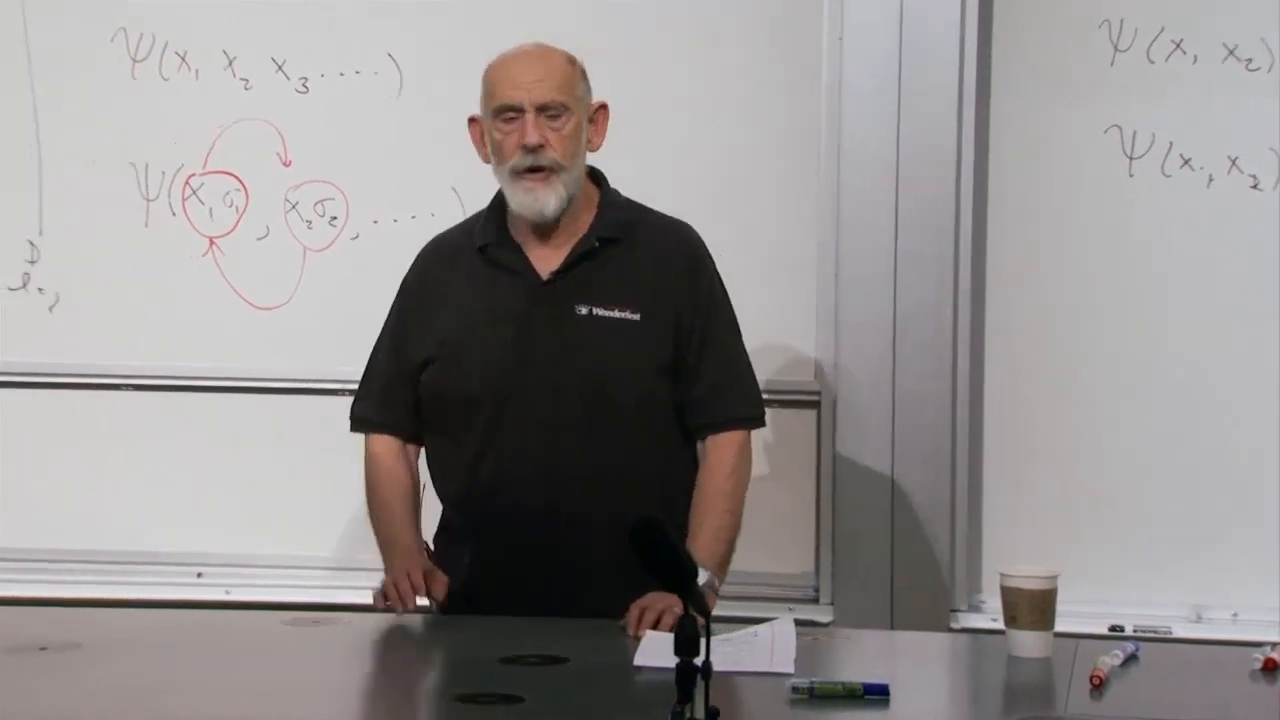
\includegraphics[width=0.9\linewidth]{lecture_05_frame_03.png}
\caption{При обмене двух тождественных частиц переставляются их полные координатно--спиновые метки. Бозонное состояние не меняется, тогда как фермионное меняет знак.}
\lectureframe{00:35:25}
\end{figure}

Это разные применения линейности. Для одной частицы
\begin{equation}
\alpha\psi_0(x)+\beta\psi_1(x)
\end{equation}
— это суперпозиция двух альтернатив. Для двух частиц
\begin{equation}
\psi_0(x_1)\psi_1(x_2)
\end{equation}
— это произведение, задающее амплитуду на пространстве с двумя координатами частиц. Симметризация или антисимметризация объединяет это произведение с соответствующим ему членом, полученным перестановкой частиц.

\begin{classroomqa}
\lecturetimestamp{00:36:13}
\audiencequestion{Порождает ли перестановка частиц интерференционный эффект?}
\lecturerresponse{Да. Исчезновение фермионной амплитуды для одного и того же состояния можно понять как деструктивную интерференцию между двумя вкладами, связанными перестановкой частиц.}
\end{classroomqa}

\begin{classroomqa}
\lecturetimestamp{00:37:13}
\audiencequestion{Вывел ли Паули правило запрета с помощью того же самого аргумента симметрии?}
\lecturerresponse{Паули исходил из эмпирического факта и нашёл математический формализм, в котором его можно было выразить. Поначалу он не выводил правило запрета из более фундаментальной теории.}
\end{classroomqa}

Антисимметрия даёт математический формализм, в котором выражается эмпирическое правило запрета.

\begin{classroomqa}
\lecturetimestamp{00:39:01}
\audiencequestion{Связана ли интерференция при перестановке частиц с интерференцией между альтернативными путями?}
\lecturerresponse{Да. В одной истории две частицы проходят, не пересекаясь, тогда как в другой они пересекаются и приходят в конечные точки друг друга. Для бозонов амплитуды складываются, а для фермионов могут взаимно уничтожаться.}
\end{classroomqa}

Перестановка даёт первый знак минус. Вращение даёт второй.

\section{Второй знак минус: вращение на \texorpdfstring{\(2\pi\)}{2 pi}}

Полный поворот, по-видимому, ничего не делает. Любое обычное геометрическое направление возвращается к исходному после угла \(2\pi\). Однако возвращаться обязаны вероятности и средние значения. Сам вектор состояния может вернуться с общей фазой, как и при перестановке.

\begin{classroomqa}
\lecturetimestamp{00:42:12}
\audiencequestion{Какая ось используется для вращения, и является ли генератором орбитальный момент импульса, спин или и то и другое?}
\lecturerresponse{Можно выбрать внешнюю ось; ниже в этом качестве берётся ось \(z\). Генератором служит полный момент импульса, включающий как орбитальный, так и спиновый вклады. Сам спин не обязан быть направлен вдоль выбранной оси.}
\end{classroomqa}

\editorialnote{В формулах для момента импульса в этом обсуждении используется \(\hbar=1\), поэтому \(m\) является безразмерным собственным значением \(J_z\).}

Пусть \(\psi(\theta)\) обозначает состояние, получаемое, когда параметр вращения проходит угол \(\theta\). В используемой здесь конвенции
\begin{equation}
J_z\psi(\theta)
=
-i\frac{\partial}{\partial\theta}\psi(\theta).
\end{equation}
Для состояния с определённым \(J_z\)
\begin{equation}
J_z\psi(\theta)=m\psi(\theta).
\end{equation}
Объединяя эти уравнения, получаем
\begin{equation}
-i\frac{\partial}{\partial\theta}\psi(\theta)
=
m\psi(\theta),
\end{equation}
с решением
\begin{equation}
\psi(\theta)=e^{im\theta}\psi(0).
\end{equation}

Допустимые значения \(m\) — целые или полуцелые. Поэтому
\begin{equation}
\psi(2\pi)
=
\begin{cases}
+\psi(0), & m\in\mathbb Z,\\[4pt]
-\psi(0), & m\in\mathbb Z+\tfrac12.
\end{cases}
\end{equation}
После ещё одного полного оборота
\begin{equation}
\psi(4\pi)=\psi(0)
\end{equation}
в обоих случаях. Это и есть второй знак минус: состояние из мультиплета с полуцелым моментом импульса меняет знак при вращении на \(2\pi\).

Знак не меняет \(\lvert\psi\rvert^2\), так что, когда он умножает всё состояние целиком, его не видно. Тем не менее вращение на \(2\pi\) не представляется тождественным оператором для состояния с полуцелым спином. Различие становится наблюдаемым, когда этот знак задаётся относительно другой когерентной амплитуды.

\section{Пути \texorpdfstring{\(2\pi\) и \(4\pi\)}{2 pi и 4 pi}}

Различие между \(2\pi\) и \(4\pi\) можно сделать наглядным без дальнейшей алгебры. Возьмите чашку в одну руку и поверните её на один полный оборот, не выпуская. Чашка возвращается к своей исходной ориентации, но рука оказывается перекрученной. Продолжите до второго полного оборота, и руку можно будет вернуть в исходное положение, не поворачивая чашку обратно.

В родственной конструкции сферу помещают внутрь коробки и соединяют её с коробкой нитями. Поворот сферы на \(2\pi\) оставляет нити спутанными. В обычном трёхмерном пространстве спутывание, связанное с поворотом на \(4\pi\), можно распутать. Существенна не просто конечная ориентация сферы, а путь, пройденный в пространстве вращений.

\begin{classroomqa}
\lecturetimestamp{00:54:22}
\audiencequestion{Если сферу дважды повернуть вокруг одной и той же оси, можно ли действительно распутать нити? Требует ли это ещё одного пространственного измерения?}
\lecturerresponse{Путь \(4\pi\) можно распутать в обычном трёхмерном пространстве. Время параметризует движение; это не ещё одно пространственное направление. Путь \(2\pi\) таким образом распутать нельзя, тогда как путь \(4\pi\) — можно.}
\end{classroomqa}

Эти демонстрации различают нетривиальный путь \(2\pi\) и распутываемый путь \(4\pi\), не развивая формальной теории группы вращений.

\section{Перестановка и вращение в представлении с ремнём}

Теперь два знака минус стоят рядом. Перестановка двух тождественных фермионов меняет знак их совместной волновой функции. Поворот состояния с полуцелым спином на \(2\pi\) тоже меняет его знак. Ремень даёт геометрическую связь между этими двумя операциями.

Расположите ремень так, чтобы два его нижних конца были переставлены местами. С другой точки зрения, тот же ремень несёт перекрут на \(2\pi\). Выполнение перестановки вместе с вращением на \(2\pi\) убирает перекрут и оставляет ремень без него. Комбинированный процесс можно непрерывно свести к тождественному преобразованию.\footnote{Наблюдение о перестановке--вращении в лекции приписывается David Finkelstein. В исходной записи не указана конкретная публикация, поэтому имя сохранено здесь только в качестве такой атрибуции.}

\begin{classroomqa}
\lecturetimestamp{01:01:12}
\audiencequestion{Не является ли это лишь утверждением о том, как ремень вложен в пространство, а не утверждением о топологии частиц?}
\lecturerresponse{Ремень можно интерпретировать как историю частиц в пространстве-времени. Если время направлено вверх, то поперечное сечение через него даёт частицеподобные объекты. Создаются пары, один объект поворачивается на \(2\pi\), и два тождественных объекта обмениваются местами. В этой истории фазы вращения и перестановки взаимно компенсируются.}
\end{classroomqa}

Эта история явно показывает учёт фаз. Начните с состояния без частиц. В двух разнесённых местах создайте пару частица--античастица, так что в промежуточный момент имеются четыре частицы. Поверните одну частицу на \(2\pi\), одновременно переставляя местами две тождественные частицы в другом месте конфигурации. Полную историю можно деформировать в элементарную историю, в которой пара создаётся, а затем аннигилирует. В обсуждаемом учёте знаков у этой тривиальной истории нет дополнительной фазы. Если \(\eta_{\mathrm{rot}}\) и \(\eta_{\mathrm{ex}}\) обозначают два этих знака, то описанную словами компенсацию можно кратко записать так\footnote{Это фазовое уравнение фиксирует компенсацию, описанную с 01:06:50 по 01:07:18; в лекции эта конструкция подаётся как наводящая на мысль, а не как строгое доказательство.}
\begin{equation}
\eta_{\mathrm{rot}}\eta_{\mathrm{ex}}=1.
\end{equation}

\begin{classroomqa}
\lecturetimestamp{01:03:34}
\audiencequestion{Можно ли связать перестановку с вращениями, повернув каждую из двух частиц на \(\pi\), а затем переориентировав их?}
\lecturerresponse{Эта конструкция может отражать родственную математику, но в ней используются два отдельных вращения на \(\pi\). Анализируемый здесь процесс содержит одно вращение на \(2\pi\), так что эти два аргумента не тождественны.}
\end{classroomqa}

Аргумент зависит от возможности создавать и аннигилировать частицеподобные объекты. В теории, чьи частицы были бы вечными, он не имел бы такой формы. Он также не предлагается как стандартное доказательство теоремы о спине--статистике. Его цель — показать топологическую причину того, почему знаки перестановки и вращения согласуются.

\section{Сгустки, зеркальные образы и аннигиляция}

Эту конструкцию можно повторить для локализованных конфигураций полей. Предположим, что одно или несколько полей почти всюду принимают свои вакуумные значения, но в малой области имеют ненулевые профиль и структуру. Такая локализованная конфигурация — сгусток.

Теперь постройте вторую конфигурацию как подходящий зеркальный образ первой. Одну назовите частицей, другую — античастицей. Сблизьте их. Соответствующие части конфигураций поля встречаются и взаимно гасят друг друга. На промежуточной стадии некоторые части сгустков, возможно, уже исчезли, тогда как другие ещё остаются. Продолжение деформации убирает оставшуюся структуру и возвращает поля к вакуумной конфигурации. Два противоположно направленных перекрута ремня дают ту же картину: сдвиньте их вместе, и они раскрутятся.

Этот процесс можно пустить в обратную сторону. Пустое пространство может породить сгусток и его зеркального партнёра. Можно создать две такие пары, повернуть один сгусток на \(2\pi\), переставить местами два тождественных сгустка и затем снова аннигилировать эти пары. Тогда действует та же компенсация перестановки--вращения. Это по-прежнему эвристическое расширение конструкции, а не теорема о каждом локализованном возбуждении.

\begin{classroomqa}
\lecturetimestamp{01:11:30}
\audiencequestion{Существуют ли физические реализации этих сгусткоподобных конфигураций поля?}
\lecturerresponse{Да. Примеры включают ядра в описаниях скирмионного типа, магнитные монополи и другие частицеподобные возбуждения полей.}
\end{classroomqa}

Именно картина зеркального сгустка делает это обобщение понятным. Существенно не то, что объект изначально был элементарной точечной частицей, а то, что частицеподобное возбуждение и его партнёр могут быть созданы, сближены и аннигилированы непрерывным образом. Это свойство и мотивирует более общее соотношение между поведением при вращении и при обмене.

\begin{classroomqa}
\lecturetimestamp{01:16:12}
\audiencequestion{Означает ли спин 1/2, что состояние накапливает только половину обычной фазы вращения?}
\lecturerresponse{Фаза в этом соглашении равна \(e^{im\theta}\). При полуцелом \(m\) поворот на \(2\pi\) даёт \(-1\), тогда как поворот на \(4\pi\) даёт \(+1\).}
\end{classroomqa}

\section{Глобальный знак и нулевой эксперимент}

Можно ли наблюдать минус-знак от поворота на \(2\pi\)? Начнём с эксперимента, в котором это невозможно. Удержите электрон в магнитном поле, дайте его спину следовать за полем, пока установка медленно поворачивается на \(2\pi\), а затем выпустите электрон в интерференционную установку. Сравните это с той же процедурой без поворота.

Поворот изменяет состояние следующим образом:
\begin{equation}
\psi\longmapsto-\psi,
\end{equation}
но минус-знак умножает всё состояние целиком. Все вероятности остаются неизменными, поэтому итоговая интерференционная картина не сохраняет никаких сведений о том, был ли предварительный поворот. Это нулевой эксперимент: общей фазе не с чем интерферировать.

\begin{classroomqa}
\lecturetimestamp{01:20:01}
\audiencequestion{Почему поворот магнитного поля нужно выполнять медленно?}
\lecturerresponse{Спин должен продолжать следовать за вращающимся магнитным полем. Если поле вращать слишком быстро, спин перестанет за ним следовать.}
\end{classroomqa}

\section{Один электрон в двух когерентных ветвях}

Знак становится наблюдаемым, когда его делают относительным. Пропустите один электрон через делитель пучка. Часть его волновой функции идёт по одному пути, а часть — по другому:
\begin{equation}
\psi(x)=\psi_1(x)+\psi_2(x).
\end{equation}
Это один электрон, а не два электрона. Он находится в когерентной суперпозиции двух альтернатив. Это различие нужно ясно сохранять: два пакета не являются двумя независимыми частицами.

Направьте два пакета в отдельные области, содержащие магнитные поля. Поверните поле в одной области на \(2\pi\), оставив поле в другой без изменения. Для состояния с полуцелым спином,
\begin{equation}
\psi_1(x)+\psi_2(x)
\longmapsto
\psi_1(x)-\psi_2(x),
\end{equation}
где метка повёрнутой ветви выбрана равной \(2\). Теперь знак является относительным. Когда позднее два пакета перекроются, сложение заменится вычитанием. Точка конструктивной интерференции может превратиться в точку деструктивной интерференции или даже в узел.

\begin{classroomqa}
\lecturetimestamp{01:23:46}
\audiencequestion{Что именно поворачивается, если есть только один электрон, но две ветви волновой функции?}
\lecturerresponse{Электрон находится в когерентной суперпозиции двух локализованных альтернатив. Одна ветвь поворачивается, а другая — нет. Если открыть ящики, чтобы узнать, какая из альтернатив реализовалась, это измерение разрушит интерференцию.}
\end{classroomqa}

Открытие ящиков обнаружило бы только один электрон — в одном ящике или в другом. Без этого измерения обе амплитуды остаются в состоянии. При повторении эксперимента интерференционная картина накапливается по одному событию детектирования за раз. В узле, созданном относительным минус-знаком, ни один электрон не детектируется.

\section{Магнитная прецессия и двухщелевая интерференция}

Более практичная схематическая постановка заменяет очень медленный эксперимент с ящиками. Разделите когерентную электронную волну на два пути. На одном пути пропустите электрон через магнитную область так, чтобы его спин сначала был поперечен полю. Затем спин прецессирует. Подбирая напряжённость поля и время пролёта, можно добиться, чтобы спин в этой ветви совершил один полный \(2\pi\)-оборот, тогда как другая ветвь не испытывает такого оборота.\footnote{В лекции сказано, что связанный с этим эксперимент со спинорной фазой был выполнен и что его принцип описан, но в исходной записи не указаны ни статья, ни конкретная установка. Поэтому изложение здесь ограничено конструкцией, данной в лекции.}

\begin{classroomqa}
\lecturetimestamp{01:27:05}
\audiencequestion{Как можно определить путь одиночного электрона?}
\lecturerresponse{Это нельзя определить, не испортив эксперимент. Любое измерение, регистрирующее, по какому пути прошёл электрон, разрушает интерференцию.}
\end{classroomqa}

\begin{classroomqa}
\lecturetimestamp{01:27:50}
\audiencequestion{Что именно представляет собой ветвь волновой функции и как делитель создаёт две ветви?}
\lecturerresponse{Ветвь — это волновой пакет, локализованный вдоль одного пути. Делитель превращает входящую волну в два пространственно разделённых пакета, а электрические или магнитные поля могут направлять эти пакеты по разным путям.}
\end{classroomqa}

Если не считать магнитной области, это двухщелевой эксперимент. Падающая электронная волна разделяется на два пакета. Выходящие волны расплываются в общую область детектирования, где их амплитуды перекрываются. При отсутствии относительного поворота центральные амплитуды могут складываться. Поворот спина на \(2\pi\) на одном из путей меняет знак одной амплитуды и может привести к взаимному сокращению тех же вкладов.

\begin{classroomqa}
\lecturetimestamp{01:30:46}
\audiencequestion{Как может возникать интерференция, если электрон проходит через разные трубки или щели?}
\lecturerresponse{Окончательное детектирование не выявляет путь. Две выходящие волновые амплитуды расплываются и перекрываются на детекторе. Попытка посмотреть, какой путь был пройден, разрушила бы интерференцию.}
\end{classroomqa}

\begin{classroomqa}
\lecturetimestamp{01:33:22}
\audiencequestion{Должен ли диаметр трубки или щели быть сравним с длиной волны электрона?}
\lecturerresponse{Для буквальной реализации двух щелей, основанной на дифракции, отверстие должно быть достаточно малым, чтобы вызвать нужное расплывание. Описываемая установка носит схематический характер, а не является практической конструкцией.}
\end{classroomqa}

\begin{classroomqa}
\lecturetimestamp{01:33:44}
\audiencequestion{Оставил бы соответствующий поворот поляризации фотонов на \(2\pi\) интерференционную картину неизменной?}
\lecturerresponse{Да. Фотоны имеют целый спин, поэтому полный поворот на \(2\pi\) не вводит фермионный минус-знак.}
\end{classroomqa}

\begin{classroomqa}
\lecturetimestamp{01:34:12}
\audiencequestion{В чём состоит небольшое отклонение практического эксперимента от идеализированной версии?}
\lecturerresponse{В идеальной конструкции спин поворачивается адиабатически. В практическом описании электрон проходит через магнитную область, и его спин прецессирует быстрее, но измеряемая фаза всё равно остаётся фазой, связанной с поворотом на \(2\pi\).}
\end{classroomqa}

Медленная схема выделяет саму идею, обеспечивая, что спин следует за полем без дополнительной динамики. Схема с прецессией динамически приводит к тому же относительному знаку. В любом варианте два пути должны перестать быть различимыми, прежде чем сможет появиться интерференционная картина.

\begin{classroomqa}
\lecturetimestamp{01:36:15}
\audiencequestion{Должны ли две ветви быть вновь объединены после делителя?}
\lecturerresponse{Да. Возникающие волновые пакеты должны перекрыться или расплыться в общую область детектирования, чтобы их амплитуды могли образовать интерференционную картину.}
\end{classroomqa}

\begin{classroomqa}
\lecturetimestamp{01:38:12}
\audiencequestion{Является ли этот эксперимент с поворотом одного электрона следствием принципа запрета Паули?}
\lecturerresponse{Нет. Здесь имеется только один электрон. Эксперимент измеряет спинорную фазу при вращении, а не запрет на нахождение двух фермионов в одном состоянии.}
\end{classroomqa}

\section{Интерференция при обмене и относительное вращение}

Обменный знак можно было бы выявить тем же общим методом, хотя предлагаемая установка сложнее. Начните с двух электронов и разделите их совместную волновую функцию на две когерентные ветви. Электронов по-прежнему только два, а не четыре: пара следует либо одной альтернативе, либо другой. Поменяйте два электрона местами в одной ветви, а в другой не обменивайте их. После того как ветви снова сведены вместе, фермионный знак обмена проявится как относительная фаза и может изменить интерференцию.

В последнем предложенном эксперименте два минус-знака сравниваются напрямую. Одна ветвь приобретает фермионную фазу обмена, тогда как другая приобретает соответствующую фазу вращения на \(2\pi\). Обе фазы равны \(-1\), так что относительный эффект компенсируется.\footnote{Запись между 01:40:26 и 01:41:15 ясно указывает на фазу обмена, фазу вращения на \(2\pi\) и их компенсацию, но точное приписывание вращения не удаётся восстановить по доступной записи речи.} В лекции это представлено как предлагаемый мысленный эксперимент, и сказано, что, насколько было известно лектору, он не был осуществлён.

\begin{classroomqa}
\lecturetimestamp{01:41:34}
\audiencequestion{Ставило бы наблюдение обменной фазы под вопрос неразличимость двух электронов?}
\lecturerresponse{Нет. Квантовая неразличимость тоньше, чем классическая тождественность. Она допускает, что вектор состояния меняет знак при обмене, хотя никакая наблюдаемая метка не различает частицы.}
\end{classroomqa}

Есть еще одна последняя оговорка. Поворот всего изолированного мира на \(2\pi\) дал бы лишь общую фазу, и никакой внутренний эксперимент не мог бы ее обнаружить. В обнаружимом эксперименте одна когерентная ветвь поворачивается относительно другой. Поэтому наблюдается не абсолютный знак, а интерференция, возникающая из-за относительного знака.

\chapter{Осцилляторы, числа заполнения и первое квантовое поле}

Квантовая теория поля — это наш базовый формализм для практически всей известной негравитационной физики. Это утверждение не следует путать с утверждением, будто любую задачу можно решить. Атом водорода поддаётся рассмотрению; когда мы переходим к атому вроде бора, вычисление уже становится намного труднее, а человек находится далеко за пределами любых реалистичных вычислений в теории поля. Формализм может быть фундаментальным, тогда как его уравнения остаются подавляюще трудными.

Поэтому мы войдём в предмет самым элементарным возможным способом. Эту область иногда называют \emph{вторичным квантованием}, но само название мало что скажет, пока мы не построим нужный аппарат. Кратчайший путь начинается не с релятивистского поля, а с гармонического осциллятора. Пружины здесь не главное. Важна алгебра операторов повышения и понижения. Когда эта алгебра повторяется для многих мод, оператор повышения перестаёт означать просто ``поднять осциллятор на один уровень'' и начинает буквально означать ``создать частицу.''

\section{Осциллятор как алгебра}

Для одного осциллятора пусть \(a^\dagger\) повышает возбуждение, а \(a\) понижает его. Обозначения \(a_+\) и \(a_-\) равносильны, но запись с кинжалом предвосхищает язык, используемый в теории поля. Нижайшее состояние удовлетворяет
\begin{equation}
a|0\rangle=0,
\end{equation}
а оператор числа имеет вид
\begin{equation}
N=a^\dagger a,
\qquad
N|n\rangle=n|n\rangle.
\end{equation}
Эти два лестничных оператора эрмитово сопряжены друг с другом, и их основной коммутатор равен
\begin{equation}
[a,a^\dagger]=1.
\label{eq:l06-single-commutator}
\end{equation}
Эта небольшая алгебра почти исчерпывает всё содержание осциллятора.

Операторы \(a\) и \(a^\dagger\) можно получить как подходящие линейные комбинации координаты и импульса. Точное соглашение зависит от нормировки \(x\), \(p\), \(m\) и \(\omega\); полезное инвариантное утверждение здесь состоит в том, что \(a^\dagger a\) восстанавливает квадратичный гамильтониан осциллятора с точностью до аддитивной энергии основного состояния. Поэтому
\begin{equation}
H=\hbar\omega\left(N+\frac12\right).
\end{equation}
В дальнейшем обсуждении мы отбросим постоянный член и будем работать с
\begin{equation}
H=\hbar\omega N.
\label{eq:l06-one-oscillator-hamiltonian}
\end{equation}
Частота задаёт цену одного возбуждения. Увеличение \(n\) на единицу стоит \(\hbar\omega\); уменьшение \(n\) на единицу высвобождает ту же величину.

\section{Множество независимых осцилляторов}

Теперь рассмотрим много осцилляторов и занумеруем их индексом \(i\). Это обозначение — лишь индекс, а не мнимая единица. Число мод может быть конечным или бесконечным. Наглядной моделью может служить набор независимых пружин; другой — нормальные моды идеальной скрипичной струны. В приложениях теории поля важен именно бесконечный набор.

Независимость имеет операторный смысл. Операторы, относящиеся к действительно независимым подсистемам, коммутируют. Иначе соответствующие величины нельзя было бы измерять независимо, и сами системы изначально не были бы независимыми. Поэтому имеем
\begin{align}
[a_i,a_j]&=0, \\
[a_i^\dagger,a_j^\dagger]&=0, \\
[a_i,a_j^\dagger]&=\delta_{ij}.
\label{eq:l06-many-commutators}
\end{align}
При \(i\ne j\) всё, относящееся к этим двум модам, коммутирует. При \(i=j\) последняя строка сводится к уравнению~\eqref{eq:l06-single-commutator}.

У каждого осциллятора есть свой оператор числа и, вообще говоря, своя частота:
\begin{equation}
N_i=a_i^\dagger a_i,
\qquad
H=\sum_i\hbar\omega_i N_i.
\label{eq:l06-many-hamiltonian}
\end{equation}
Одновременное собственное состояние задаётся полным списком
\begin{equation}
|n_1,n_2,n_3,\ldots\rangle,
\qquad n_i=0,1,2,\ldots.
\label{eq:l06-occupation-ket}
\end{equation}
Целое число \(n_i\) называется \emph{числом заполнения} \(i\)-го осциллятора. На этом этапе это лишь термин. Вскоре оно будет считать частицы, занимающие одночастичное состояние, и название станет буквальным.

Состояние, в котором все числа заполнения равны нулю, имеет вид
\begin{equation}
|0\rangle\equiv|0,0,0,\ldots\rangle,
\qquad a_i|0\rangle=0\quad\text{for every }i.
\label{eq:l06-oscillator-vacuum}
\end{equation}

\begin{classroomqa}
\lecturetimestamp{00:15:27}
\audiencequestion{Соответствует ли бесконечное семейство осцилляторов континууму мод системы вроде скрипичной струны?}
\lecturerresponse{Да, для идеализированной струны. Реальная струна состоит из атомов, поэтому достаточно короткие длины волн в конце концов натыкаются на микроскопическое отсечение. Тем не менее модель сплошной среды мотивирует бесконечный набор мод, используемый в теории поля.}
\end{classroomqa}

\section{Почему коэффициенты лестничных операторов — квадратные корни}

Действие \(a^\dagger\) должно переводить собственное состояние оператора \(N\) в следующее собственное состояние, но нормировка допускает коэффициент:
\begin{equation}
a^\dagger|n\rangle=c_n|n+1\rangle.
\label{eq:l06-unknown-coefficient}
\end{equation}

\begin{figure}[htbp]
\centering
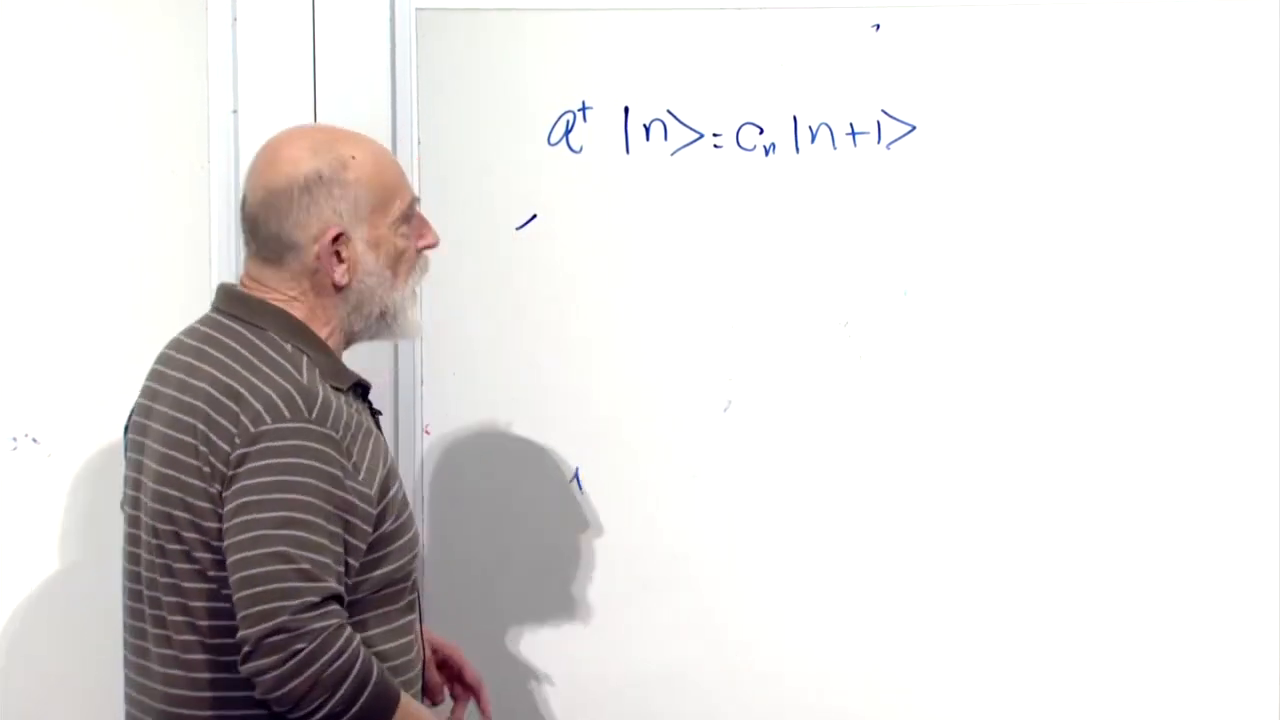
\includegraphics[width=0.9\linewidth]{lecture_06_frame_01.png}
\caption{Коэффициент лестничного оператора вводится до вывода его нормировки. Уравнение, написанное на доске, воспроизведено в уравнении~\eqref{eq:l06-unknown-coefficient}.}
\lectureframe{00:19:38}
\end{figure}

Выберем фазовое соглашение, в котором \(c_n\) вещественно. Переход к эрмитову сопряжению даёт
\begin{equation}
\langle n|a=c_n\langle n+1|.
\end{equation}
Умножая эти два соотношения и используя нормированные базисные состояния, получаем
\begin{align}
c_n^2
&=\langle n|aa^\dagger|n\rangle \\
&=\langle n|(a^\dagger a+1)|n\rangle \\
&=\langle n|(N+1)|n\rangle \\
&=n+1.
\end{align}
Следовательно,
\begin{equation}
a^\dagger|n\rangle=\sqrt{n+1}\,|n+1\rangle.
\label{eq:l06-raising-rule}
\end{equation}

\begin{classroomqa}
\lecturetimestamp{00:22:35}
\audiencequestion{Почему можно положить \(\langle n+1|n+1\rangle=1\) ещё до нахождения \(c_n\)?}
\lecturerresponse{Собственные векторы с самого начала выбираются как нормированный базис. Их нормировка не определяет нормировку \(a^\dagger|n\rangle\); именно эта оставшаяся информация и содержится в коэффициенте \(c_n\).}
\end{classroomqa}

Правило понижения получается тем же способом:
\begin{equation}
a|n\rangle=\sqrt n\,|n-1\rangle.
\label{eq:l06-lowering-rule}
\end{equation}
При \(n=0\) коэффициент автоматически обращается в нуль, так что правило включает и \(a|0\rangle=0\). Для многих мод оператор изменяет только число заполнения в своей собственной позиции:
\begin{align}
a_i^\dagger|n_1,\ldots,n_i,\ldots\rangle
&=\sqrt{n_i+1}\,|n_1,\ldots,n_i+1,\ldots\rangle, \\
a_i|n_1,\ldots,n_i,\ldots\rangle
&=\sqrt{n_i}\,|n_1,\ldots,n_i-1,\ldots\rangle.
\label{eq:l06-multimode-ladders}
\end{align}
Остальные записи не меняются.

\section{Волновая функция — не квантовое поле}

Прежде чем определять поле, нужно отделить его от привычной волновой функции. Этот переход удобно прояснить тремя противопоставлениями.

Во-первых, одночастичная волновая функция
\begin{equation}
\psi(x)=\langle x|\psi\rangle
\end{equation}
является представлением вектора состояния. Сама по себе она не является наблюдаемой. Мы измеряем положение, импульс, момент импульса и другие наблюдаемые; волновая функция задаёт амплитуды, по которым вычисляются вероятности этих исходов.

Во-вторых, многочастичная волновая функция зависит от положений всех частиц. Для двух частиц, радиус-векторы которых мы временно обозначим через \(x\) и \(y\),
\begin{equation}
\psi(x,y)=\langle x,y|\psi\rangle.
\end{equation}
Здесь \(x\) и \(y\) обозначают две разные частицы; это не декартовы \(x\)- и \(y\)-компоненты одного вектора положения. При \(N\) частицах состояние представляется как
\begin{equation}
\psi(x_1,x_2,\ldots,x_N).
\end{equation}

В-третьих, эта волновая функция описывает фиксированное число частиц. Волновая функция для 15 частиц имеет 15 аргументов положения и принадлежит 15-частичному гильбертову пространству. Сама по себе она не описывает процесс, в котором это число меняется с 15 на 14 или 16.

Квантовое поле будет обладать противоположными свойствами. Это оператор, а не состояние; оно зависит от одной пространственной точки \(x\) и действует в пространстве состояний, содержащем все секторы с разным числом частиц. Выражение ``одна точка'' означает один свободно изменяющийся вектор положения. Оно не означает, что \(x\) присвоено одно численное значение.

Есть одна оговорка, которая позже окажется важной. Поле \(\Psi(x)\), вводимое ниже, не эрмитово, поэтому само по себе оно не является наблюдаемой в строгом смысле. Его эрмитовы комбинации являются наблюдаемыми. Поэтому предварительное утверждение о том, что поле измеримо, нужно уточнить, а не отбросить: поля — это операторнозначные функции, а их эрмитовы комбинации представляют измеримые величины.

\begin{classroomqa}
\lecturetimestamp{00:36:52}
\audiencequestion{Если поле есть функция одного положения, может ли это положение изменяться? И что произошло с \(y\) в двухчастичной волновой функции?}
\lecturerresponse{Точка \(x\) пробегает всё пространство. ``Одно положение'' означает, что у оператора один пространственный аргумент, а не то, что этот аргумент фиксирован. В \(\psi(x,y)\) символы \(x\) и \(y\) обозначают положения двух частиц; эквивалентно, это \(x_1\) и \(x_2\). Это не две декартовы компоненты аргумента поля.}
\end{classroomqa}

\begin{classroomqa}
\lecturetimestamp{00:38:15}
\audiencequestion{Как связаны описание через волновую функцию с фиксированным числом частиц и полевое описание, и описывают ли они разные виды частиц?}
\lecturerresponse{Эта связь — центральная конструкция, к которой мы ещё подойдём. Частицы одного и того же вида. В этой лекции это бозоны; для фермионов требуется другая алгебра.}
\end{classroomqa}

\section{Одна частица в ящике}

Временно вернёмся к обычной одночастичной квантовой механике. Поместим частицу в одномерный ящик. Если частица только одна, различие между бозоном и фермионом несущественно: нет второй тождественной частицы, на которой можно было бы проверить обменные свойства или запрет.

Пусть
\begin{equation}
\psi_1(x),\ \psi_2(x),\ \psi_3(x),\ldots
\end{equation}
будут собственными функциями энергии. Низшая мода — это наиболее гладкая волна, обращающаяся в нуль на стенках. Следующая мода имеет один внутренний узел, а моды с большей энергией осциллируют быстрее. В идеальной бесконечной прямоугольной яме ширины \(L\) удобный нормированный базис имеет вид
\begin{equation}
\psi_i(x)=\sqrt{\frac{2}{L}}\sin\!\left(\frac{i\pi x}{L}\right),
\qquad 0<x<L.
\label{eq:l06-box-basis}
\end{equation}
Явная синусоидальная формула — стандартная реализация качественного рисунка на доске; для дальнейших рассуждений требуется лишь полный ортонормированный набор одночастичных состояний.

\begin{figure}[htbp]
\centering
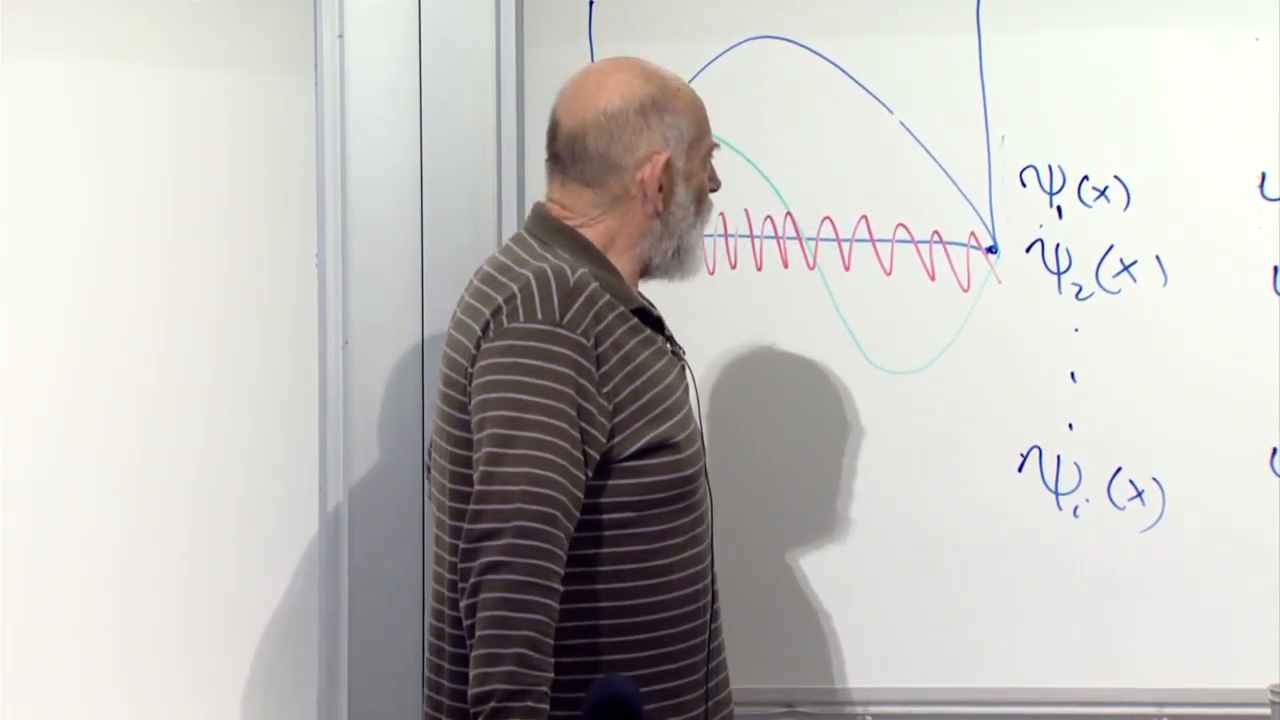
\includegraphics[width=0.9\linewidth]{lecture_06_frame_03.png}
\caption{Одночастичные моды в ящике, упорядоченные по возрастанию энергии. Первая мода не имеет внутренних узлов, вторая имеет один, а опущенные более высокие моды колеблются всё быстрее.}
\lectureframe{00:43:10}
\end{figure}

Ту же структуру можно перерисовать без того перекрытия, которое возникает на доске в аудитории:
\begin{figure}[htbp]
\centering
\begin{tikzpicture}[x=1cm,y=1cm]
  \draw[thick] (0,0) -- (0,3.8);
  \draw[thick] (7,0) -- (7,3.8);
  \draw[gray!55] (0,2.75) -- (7,2.75);
  \draw[gray!55] (0,1.35) -- (7,1.35);
  \draw[blue!75!black,thick,domain=0:7,samples=120]
    plot (\x,{2.75+0.62*sin(180*\x/7)});
  \draw[teal!70!black,thick,domain=0:7,samples=120]
    plot (\x,{1.35+0.55*sin(360*\x/7)});
  \node[right] at (7.15,3.15) {$\psi_1(x)$};
  \node[right] at (7.15,1.70) {$\psi_2(x)$};
  \node at (3.5,0.45) {$\vdots\quad \psi_i(x)$};
\end{tikzpicture}
\caption{Аккуратная реконструкция качественного наброска мод в ящике. Смещение по вертикали разделяет собственные функции для удобства чтения и не является дополнительной физической координатой.}
\end{figure}

Индекс \(i\) обозначает одночастичное состояние, а не частицу и не число узлов. В базисе ящика \(i\) оказывается на единицу больше числа внутренних узлов. Каждому состоянию соответствует энергия \(\varepsilon_i\). Следуя обозначениям лекции, мы можем записать эту энергию как \(\hbar\omega_i\), или просто \(\omega_i\) после того, как положено \(\hbar=1\).

\begin{classroomqa}
\lecturetimestamp{00:39:01}
\audiencequestion{Было ли прежнее предположение о независимости точным, и может ли индекс \(i\) обозначать возможные состояния электрона в атоме?}
\lecturerresponse{В построении с независимыми модами коммутация между различными модами точна. Индекс может обозначать одночастичные атомные состояния. Если же частицы взаимодействуют, простой гамильтониан независимых мод уже не исчерпывает всей картины.}
\end{classroomqa}

\begin{classroomqa}
\lecturetimestamp{00:40:34}
\audiencequestion{Является ли частица в ящике бозоном?}
\lecturerresponse{Может, но при одной частице статистика не имеет значения. Запрет и обмен приобретают смысл только тогда, когда имеется более одной тождественной частицы.}
\end{classroomqa}

\section{От мод в ящике к пространству Фока}

Теперь допустим в ящике любое число тождественных бозонов. Некоторое число \(n_1\) может занимать \(\psi_1\), некоторое число \(n_2\) может занимать \(\psi_2\), и так далее. Поэтому базисное состояние имеет вид
\begin{equation}
|n_1,n_2,n_3,\ldots\rangle.
\end{equation}
Это в точности то обозначение, которое уже использовалось для многих осцилляторов. Это тождество носит структурный характер: сопоставим каждому одночастичному состоянию один осциллятор и отождествим число возбуждения осциллятора с числом частиц, занимающих это состояние.

Бозоны здесь существенны, потому что каждое \(n_i\) может быть любым неотрицательным целым числом. Для фермионов каждое одночастичное состояние может быть пустым или занятым одной частицей, но никогда не двумя, так что обычную алгебру осциллятора нельзя использовать без изменений.

Операторы теперь можно определить по их действию на базис чисел заполнения. Оператор \(a_i^\dagger\) создаёт одну частицу в одночастичном состоянии \(i\); \(a_i\) уничтожает одну:
\begin{align}
a_i^\dagger|n_1,\ldots,n_i,\ldots\rangle
&=\sqrt{n_i+1}\,|n_1,\ldots,n_i+1,\ldots\rangle, \\
a_i|n_1,\ldots,n_i,\ldots\rangle
&=\sqrt{n_i}\,|n_1,\ldots,n_i-1,\ldots\rangle.
\end{align}
Это не аналогия, придуманная задним числом. Это и есть определение бозонных операторов рождения и уничтожения на этом базисе. Поскольку этот базис порождает пространство, по линейности определение задаёт их действие на любом состоянии.

\begin{classroomqa}
\lecturetimestamp{00:47:11}
\audiencequestion{Являются ли \(n_1,n_2,n_3\) квантовыми состояниями?}
\lecturerresponse{Метки \(1,2,3,\ldots\) задают одночастичные состояния. Символы \(n_1,n_2,n_3,\ldots\) — это числа частиц, занимающих эти состояния. Главная трудность обозначений состоит в том, чтобы не смешивать метку состояния с его числом заполнения.}
\end{classroomqa}

\subsection{Что делает квадратный корень}

Множитель \(\sqrt{n_i+1}\) не обозначает ни дополнительную частицу, ни отдельный физический процесс. Он обеспечивает оператору правильную нормировку и правильную алгебру. Для одной моды
\begin{align}
a a^\dagger|n\rangle
&=a\bigl(\sqrt{n+1}\,|n+1\rangle\bigr) \\
&=(n+1)|n\rangle,
\end{align}
тогда как
\begin{equation}
a^\dagger a|n\rangle=n|n\rangle.
\end{equation}
Поэтому их разность равна \(|n\rangle\), как и требуется условием \([a,a^\dagger]=1\). Очень грубо говоря, каждый из двух лестничных операторов имеет порядок \(\sqrt n\), поскольку их произведение даёт оператор числа частиц порядка \(n\).

\begin{classroomqa}
\lecturetimestamp{00:47:52}
\audiencequestion{Какой осязаемый физический смысл имеет множитель с квадратным корнем?}
\lecturerresponse{В первую очередь это математическая нормировка. Он обеспечивает, что состояния с числами заполнения нормированы, что \(a^\dagger a\) имеет собственное значение \(n\) и что лестничные операторы удовлетворяют коммутатору осциллятора. Иногда математика и есть тот смысл, который нужен.}
\end{classroomqa}

\begin{classroomqa}
\lecturetimestamp{00:52:25}
\audiencequestion{Были ли операторы рождения и уничтожения определены только через их свойства и их действие на базис?}
\lecturerresponse{Да. Определения не обязаны возникать из более первичной картины. Их ценность проверяется их следствиями. Если задать действие на полном базисе, операторы тем самым задаются на всём пространстве, и эти определения воспроизводят нужные коммутационные соотношения.}
\end{classroomqa}

\begin{classroomqa}
\lecturetimestamp{00:53:22}
\audiencequestion{Почему \(a_i\) заставляет частицу исчезнуть, а не просто переводит её в другое состояние?}
\lecturerresponse{Потому что \(a_i\) по определению понижает заполнение состояния \(i\). Полезный вопрос состоит не в том, почему определение истинно, а в том, почему оно полезно. Оно полезно потому, что испускание и поглощение требуют операторов, меняющих число частиц: фотон создаётся при испускании излучения и уничтожается при его поглощении.}
\end{classroomqa}

Пространство, порождаемое всеми состояниями с числами заполнения, есть \emph{пространство Фока}. Оно содержит вакуум, все одночастичные состояния, все двухчастичные состояния и так далее без фиксированной верхней границы:
\begin{equation}
\mathcal F=\mathcal H_0\oplus\mathcal H_1\oplus\mathcal H_2\oplus\cdots.
\label{eq:l06-fock-space}
\end{equation}
Обозначение прямой суммы явно показывает то, чего обычная \(N\)-частичная волновая функция не показывала: все секторы с разным числом частиц принадлежат одному пространству состояний.

\begin{classroomqa}
\lecturetimestamp{00:54:56}
\audiencequestion{Определяет ли задание операторов на собственных векторах чисел заполнения их действие на произвольные векторы, и следуют ли тогда коммутаторы осциллятора?}
\lecturerresponse{Именно. Векторы заполнения образуют базис, поэтому линейность распространяет определение на всё пространство Фока. Действуя на этом базисе, мы проверяем бозонные коммутационные соотношения. Каждому одночастичному состоянию соответствует один осциллятор, а его число заполнения как осциллятора равно числу частиц в этом состоянии.}
\end{classroomqa}

\subsection{Вакуум и свободный гамильтониан}

Вакуум Фока — это состояние, в котором ни в одном одночастичном состоянии нет частиц:
\begin{equation}
|0\rangle=|0,0,0,\ldots\rangle,
\qquad a_i|0\rangle=0.
\end{equation}
Слово \emph{основное состояние} здесь может вводить в заблуждение. Самое низкое \emph{одночастичное} состояние — это мода \(i=1\); в вакууме Фока нет частицы даже в этой моде. Если частица занимает низшую моду, \(a_1\) может уничтожить её и вернуть систему в вакуум.

\begin{classroomqa}
\lecturetimestamp{00:56:19}
\audiencequestion{Что такое вакуум на языке чисел заполнения? Занято ли низшее одночастичное состояние?}
\lecturerresponse{В вакууме все числа заполнения равны нулю, и он аннулируется каждым \(a_i\). Низшая одночастичная мода в вакууме не занята. Если бы она была занята, её оператор уничтожения мог бы убрать эту частицу.}
\end{classroomqa}

Для невзаимодействующих частиц полная энергия аддитивна. Если одна частица в состоянии \(i\) имеет энергию \(\hbar\omega_i\), то
\begin{align}
H
&=\sum_i \hbar\omega_i N_i \\
&=\sum_i \hbar\omega_i a_i^\dagger a_i.
\label{eq:l06-free-fock-hamiltonian}
\end{align}
Здесь возможны два эквивалентных прочтения. Это сумма энергий осцилляторов, по одному осциллятору на каждое одночастичное состояние. Это также сумма по одночастичным энергиям, каждая из которых умножена на число частиц, обладающих этой энергией.

В обозначениях теории поля \(a_i^\dagger\) обычно называется оператором рождения, а \(a_i\) — оператором уничтожения. Более старое обозначение \(a_+\) и \(a_-\) означает то же самое.

\section{Уточнения перед появлением поля}

Несколько вопросов после перерыва позволяют отличить новую осцилляторную схему учёта от обычной частицы, движущейся в осцилляторном потенциале.

\begin{classroomqa}
\lecturetimestamp{01:06:09}
\audiencequestion{Энергетические уровни частицы в ящике не равноотстоящие, так где же здесь гармонический осциллятор?}
\lecturerresponse{Одночастичные энергии \(\omega_i\) не обязаны быть равноотстоящими. Однако для каждой фиксированной моды \(i\) энергии нуля, одной, двух и трёх невзаимодействующих частиц в этой моде равны \(0,\omega_i,2\omega_i,3\omega_i\). Эта лестница заполнения и есть осциллятор. Она отлична от ситуации, когда одна частица помещена в потенциал гармонического осциллятора.}
\end{classroomqa}

\begin{classroomqa}
\lecturetimestamp{01:08:38}
\audiencequestion{Связано ли это построение с разложением Фурье?}
\lecturerresponse{Самым тесным образом. Если одночастичный базис состоит из мод импульса, то модовые функции — это синусы, косинусы или комплексные экспоненты, а \(a_i\) являются квантовыми аналогами коэффициентов Фурье. Общий базис не обязан быть тригонометрическим, но логика разложения остаётся той же.}
\end{classroomqa}

\begin{classroomqa}
\lecturetimestamp{01:09:07}
\audiencequestion{Всем ли частицам приписывается одна и та же энергия, и учтены ли взаимодействия?}
\lecturerresponse{Частицы, занимающие одно и то же одночастичное состояние, имеют одну и ту же энергию, тогда как частицы в разных состояниях, вообще говоря, имеют разные энергии. Пока частицы свободны: они не взаимодействуют. Взаимодействия добавили бы члены потенциальной энергии, так что гамильтониан уже не был бы просто аддитивной суммой в уравнении~\eqref{eq:l06-free-fock-hamiltonian}.}
\end{classroomqa}

\begin{classroomqa}
\lecturetimestamp{01:10:26}
\audiencequestion{Что стало с половиной кванта энергии нулевых колебаний в каждом осцилляторе?}
\lecturerresponse{Это аддитивная константа в гамильтониане. Константа коммутирует с любым оператором, так что она не изменяет уравнения движения Гейзенберга, а обычные негравитационные измерения зависят от разностей энергий. Для специальных целей она может иметь значение, но на построение, развиваемое здесь, не влияет.}
\end{classroomqa}

Свободная теория уже сама по себе представляет собой аппарат учёта необычайной силы. Она позволяет отслеживать не только множество частиц, но и частицы, которые меняют состояние, появляются, исчезают или существуют в суперпозициях с различным полным числом. Операторы — это не просто символы учёта, поскольку подходящие эрмитовы комбинации можно измерять, но как первая интуиция такой взгляд полезен.

\begin{classroomqa}
\lecturetimestamp{01:14:03}
\audiencequestion{Откуда исторически возникли теория поля и квантовая теория поля?}
\lecturerresponse{Краткий исторический очерк начинается с физической картины электрических и магнитных полей у Фарадея и уравнений Максвелла для классических полей. Планк ввёл кванты энергии при изучении теплового излучения; Эйнштейн отнёс квантование к самому электромагнитному полю и к квантам света. Затем Хайзенберг, Паули и особенно Дирак помогли сформировать современный операторный формализм к концу 1920-х годов. Ультрафиолетовая катастрофа и квантовое описание излучения были среди решающих ранних проблем. Это схематическая история, а не исчерпывающее распределение приоритетов.}
\end{classroomqa}

Эта историческая нить также объясняет, почему осцилляторы всё время возвращаются. Классическое излучение в полости раскладывается по нормальным модам. Квантование этих мод превращает числа их возбуждения в числа фотонов. Математические кванты, занимающие эти моды, становятся физическими частицами.

\section{Оператор бозонного поля}

Пусть \(\{\psi_i(x)\}\) — полный ортонормированный базис одночастичных волновых функций. Определим
\begin{equation}
\boxed{\Psi(x)=\sum_i a_i\,\psi_i(x)}
\label{eq:l06-field-annihilation}
\end{equation}
и его эрмитово сопряжение
\begin{equation}
\boxed{\Psi^\dagger(x)=\sum_i a_i^\dagger\,\psi_i^*(x)}.
\label{eq:l06-field-creation}
\end{equation}

\begin{figure}[htbp]
\centering
\includegraphics[width=0.9\linewidth]{lecture_06_frame_04.png}
\caption{Полные разложения по модам поля уничтожения и его эрмитова сопряжения. Уравнения~\eqref{eq:l06-field-annihilation} и \eqref{eq:l06-field-creation} сохраняют в наборе ту же структуру операторов и комплексного сопряжения.}
\lectureframe{01:25:15}
\end{figure}

Для любого фиксированного положения \(x\) каждое \(\psi_i(x)\) — обычное комплексное число. Всё операторное содержание заключено в \(a_i\) и \(a_i^\dagger\). Когда \(x\) меняется, мы получаем другой оператор в каждой точке пространства. Именно в этом точном смысле \(\Psi\) является операторнозначной функцией.

Если базисные функции — плоские волны, то уравнения~\eqref{eq:l06-field-annihilation} и \eqref{eq:l06-field-creation} представляют собой квантовые разложения Фурье: классические коэффициенты Фурье стали операторами. В ящике базисом вместо этого могут служить синусные функции из уравнения~\eqref{eq:l06-box-basis}. Подходит любой полный ортонормированный одночастичный базис.

Ни \(\Psi\), ни \(\Psi^\dagger\) не является эрмитовым. Наблюдаемые поля можно строить из эрмитовых комбинаций, таких как
\begin{equation}
\Psi(x)+\Psi^\dagger(x),
\qquad
i\bigl(\Psi^\dagger(x)-\Psi(x)\bigr),
\end{equation}
а наблюдаемые плотности позже будут строиться из произведений, таких как \(\Psi^\dagger(x)\Psi(x)\). Сейчас задача прежде всего понять, что делают два базовых поля.

\begin{classroomqa}
\lecturetimestamp{01:23:14}
\audiencequestion{Как левая часть может быть оператором, если модовые функции справа — обычные волновые функции?}
\lecturerresponse{Функции \(\psi_i(x)\) после выбора \(x\) являются числами. Множители \(a_i\) — операторы. Число, умноженное на оператор, даёт оператор, и потому сумма тоже является оператором. Изменяя \(x\), мы получаем всё семейство операторов.}
\end{classroomqa}

\section{Что делает поле}

Поле уничтожения сразу уничтожает вакуум:
\begin{equation}
\Psi(x)|0\rangle
=\sum_i\psi_i(x)a_i|0\rangle
=0.
\label{eq:l06-field-kills-vacuum}
\end{equation}
Поле рождения делает нечто гораздо более содержательное.

Пусть \(|i\rangle\) обозначает одночастичное состояние с волновой функцией
\begin{equation}
\langle x|i\rangle=\psi_i(x).
\end{equation}
Из полноты одночастичного базиса следует
\begin{equation}
\sum_i|i\rangle\langle i|=1.
\label{eq:l06-completeness}
\end{equation}
Применим это тождество к собственному состоянию координаты:
\begin{align}
|x\rangle
&=\sum_i|i\rangle\langle i|x\rangle \\
&=\sum_i\psi_i^*(x)|i\rangle.
\label{eq:l06-position-expansion}
\end{align}
На языке Фока одночастичное модовое состояние имеет вид
\begin{equation}
|i\rangle=a_i^\dagger|0\rangle.
\end{equation}
Подставляя это в уравнение~\eqref{eq:l06-position-expansion},
\begin{align}
|x\rangle
&=\sum_i\psi_i^*(x)a_i^\dagger|0\rangle \\
&=\Psi^\dagger(x)|0\rangle.
\label{eq:l06-local-creation}
\end{align}
Следовательно, \(\Psi^\dagger(x)\) создаёт частицу, локализованную в точке \(x\), тогда как \(\Psi(x)\) удаляет там одну частицу. Собственное состояние координаты локализовано дельта-функцией и является обобщённым, ненормируемым состоянием; физическую локализованную частицу получают, свёртывая поле с нормируемым волновым пакетом.\editorialnote{В лекции используется идеализированный язык собственных состояний координаты. Уточнение о волновом пакете фиксирует стандартный математический смысл, не изменяя аргумента.}

\begin{classroomqa}
\lecturetimestamp{01:36:26}
\audiencequestion{Где содержится информация о том, какого вида частица создаётся? Является ли состояние в \(x\) локализованным дельта-функцией?}
\lecturerresponse{Каждому виду частиц сопоставляется отдельное поле, так что тождество частицы задаётся тем, какое поле используется. Аргумент \(x\) указывает, где она создаётся. В идеальном координатном базисе создаваемое состояние дельта-функционально локализовано.}
\end{classroomqa}

К примерам бозонных видов относятся фотоны, гравитоны, бозоны Хиггса и глюоны, хотя реалистические поля также несут внутренние индексы. Даже для фотонов нужны поляризационные метки. Упрощённая нотация скалярного поля опускает эти дополнительные метки, чтобы сам принцип создания оставался наглядным.

\subsection{Вакуум — не нулевой вектор}

Уравнение
\begin{equation}
\Psi(x)|0\rangle=0
\end{equation}
содержит два очень разных объекта, обозначаемых нулём. Кет \(|0\rangle\) — это вакуум: нормированное физическое состояние, для которого
\begin{equation}
\langle0|0\rangle=1.
\end{equation}
Результат справа — нулевой вектор. Его норма равна нулю; его нельзя нормировать, и он не представляет физического состояния.

Различие становится особенно ясным при сложении. Прибавление нулевого вектора к одночастичному состоянию ничего не меняет. Прибавление вакуума к одночастичному состоянию даёт настоящую суперпозицию секторов с разным числом частиц. При нормированных коэффициентах
\begin{equation}
|\chi\rangle=\frac{1}{\sqrt2}\bigl(|0\rangle+|1\rangle\bigr)
\end{equation}
имеет равные вероятности состояний с нулём и с одной частицей. Это не то же самое, что \(|1\rangle\).

\begin{classroomqa}
\lecturetimestamp{01:37:23}
\audiencequestion{Если в \(x\) нет частицы, не делает ли \(\Psi(x)\) просто ничего? Что означает, что результат равен нулю?}
\lecturerresponse{Нет, исходное состояние не возвращается. Результатом является нулевой вектор. Вакуум — это нормированное состояние, описывающее пустое пространство; нулевой вектор имеет нулевую длину и не описывает никакого физического состояния. Любой оператор, действуя на нулевой вектор, возвращает нулевой вектор.}
\end{classroomqa}

\begin{classroomqa}
\lecturetimestamp{01:39:00}
\audiencequestion{Что происходит, если к одночастичному состоянию прибавить вакуум, а не нулевой вектор?}
\lecturerresponse{Получается суперпозиция с амплитудами для разных чисел частиц. Напротив, прибавление нулевого вектора оставляет одночастичное состояние неизменным. Символ в \(|0\rangle\) обозначает нулевое заполнение; он не означает нулевой вектор.}
\end{classroomqa}

\begin{classroomqa}
\lecturetimestamp{01:41:56}
\audiencequestion{Имеет ли значение порядок модовой функции и её оператора рождения или уничтожения в разложении поля? Являются ли модовые функции комплексными?}
\lecturerresponse{Модовая функция — обычное число и потому коммутирует с любым оператором, так что порядок не имеет значения. Вообще говоря, модовые функции могут быть комплексными; будет ли выбранный базис вещественным или комплексным, зависит от одночастичной задачи Schr\"odinger.}
\end{classroomqa}

\subsection{Две частицы и возникновение бозонной симметрии}

Чтобы создать одну частицу в \(x\) и другую в \(y\), нужно подействовать дважды:
\begin{equation}
|x,y\rangle
=\Psi^\dagger(y)\Psi^\dagger(x)|0\rangle.
\label{eq:l06-two-particle-state}
\end{equation}
Эти точки могут совпадать или различаться. Поскольку лежащие в основе операторы рождения коммутируют,
\begin{align}
[\Psi^\dagger(x),\Psi^\dagger(y)]
&=\sum_{i,j}\psi_i^*(x)\psi_j^*(y)
[a_i^\dagger,a_j^\dagger] \\
&=0.
\end{align}
отсюда следует, что
\begin{equation}
\Psi^\dagger(y)\Psi^\dagger(x)|0\rangle
=\Psi^\dagger(x)\Psi^\dagger(y)|0\rangle.
\label{eq:l06-boson-exchange}
\end{equation}
Перестановка порядка двух частиц ничего не меняет. Это и есть бозонная обменная симметрия. Поэтому мы могли бы начать с алгебры осциллятора и \emph{вывести}, что частицы, построенные из коммутирующих операторов рождения, являются бозонами. Для фермионов вместо этого потребуются антикоммутирующие операторы.

\begin{classroomqa}
\lecturetimestamp{01:42:37}
\audiencequestion{Как добавить вторую частицу к одночастичному состоянию?}
\lecturerresponse{Примените ещё одно поле рождения. Чтобы добавить её в \(y\), подействуйте \(\Psi^\dagger(y)\) слева от \(\Psi^\dagger(x)\). Результатом будет двухчастичное состояние из уравнения~\eqref{eq:l06-two-particle-state}.}
\end{classroomqa}

\begin{classroomqa}
\lecturetimestamp{01:46:04}
\audiencequestion{Полностью ли эквивалентна коммутативность двух полей рождения симметризации двухчастичного состояния?}
\lecturerresponse{Да. Она делает состояние с одной частицей в \(x\) и одной в \(y\) тождественным состоянию, полученному после обмена меток. Это определяющее обменное свойство тождественных бозонов.}
\end{classroomqa}

\begin{classroomqa}
\lecturetimestamp{01:46:32}
\audiencequestion{Означает ли это, что частицы в точках \(x\) и \(y\) должны быть бозонами одного и того же вида?}
\lecturerresponse{Да. Аргументы \(x\) и \(y\) — это координаты, тогда как одно поле описывает один вид частиц. Для различных видов, а также для дополнительных меток, таких как две поляризации фотона, требуются отдельные компоненты поля.}
\end{classroomqa}

\section{Почему важно переменное число частиц}

Если бы в задаче всегда было ровно 37 частиц, язык полей был бы лишь необязательным средством учёта. Его подлинная сила проявляется, когда частицы могут испускаться и поглощаться, и особенно когда само число частиц является квантовой переменной. Пространство Фока допускает состояния вида
\begin{equation}
|\Phi\rangle
=c_0|0\rangle+c_1|1\rangle+c_2|2\rangle+\cdots,
\qquad
\sum_{n=0}^{\infty}|c_n|^2=1.
\end{equation}
Важный пример — лазерное поле: вообще говоря, это не состояние с одним точно определённым числом фотонов, а суперпозиция многих секторов с различным числом фотонов.

Теперь связь между частицами и полями выражена явно. Операторы мод подсчитывают частицы в собственных состояниях энергии и изменяют их число; поле объединяет эти операторы с полным набором волновых функций, так что частицы можно создавать или уничтожать в заданных точках. Алгебра гармонических осцилляторов стала элементарным языком бозонного квантового поля.

\chapter{От частиц к простому квантовому полю}

Построим простое квантовое поле еще раз, но под несколько иным углом зрения. К квантовой теории поля ведут два пути. Можно начать с частиц и понять, почему поле является для них естественным языком, или начать с волнового поля и понять, почему его возбуждения квантуются. Оба пути полезны. Здесь мы придерживаемся первого.

Обычная квантовая механика может описывать одну частицу, две частицы или любое другое фиксированное число. Природа не соблюдает этого ограничения. Число фотонов в комнате меняется всякий раз, когда источники света испускают или поглощают излучение. Нестабильные частицы распадаются. При бета-распаде, например,
\begin{equation}
n\longrightarrow p+e^-+\bar{\nu}_e,
\end{equation}
так что одновременно меняются численности нескольких видов частиц. Поэтому нам нужна одна квантовая механика, достаточно большая, чтобы охватывать любое возможное число заполнения и, в конечном счете, процессы перехода между ними.

Пока что мы сильно упростим задачу. Есть один вид нерелятивистской частицы. Сначала мы расширим пространство ее состояний так, чтобы в нем могло содержаться любое число частиц, и лишь затем обсудим большее число видов, релятивистский случай, рассеяние и распад. Никакая часть математики здесь не является особенно трудной, но смена точки зрения абстрактна. Стоит продвигаться достаточно медленно, чтобы обозначения не скрыли саму идею.

\section{Одночастичная отправная точка}

Начнем с одной частицы в состоянии \(|\psi\rangle\). Ее волновая функция в координатном представлении имеет вид
\begin{equation}
\psi(x)=\langle x|\psi\rangle.
\label{eq:l07-wavefunction}
\end{equation}
Эта строчная \(\psi\) есть обычная комплекснозначная функция. Это еще не квантовое поле и не оператор в пространстве состояний многих частиц.

Согласно правилу Борна,
\begin{equation}
\rho_\psi(x)=|\psi(x)|^2=\psi^*(x)\psi(x)
\label{eq:l07-born-density}
\end{equation}
есть плотность вероятности обнаружить частицу в точке \(x\). Для нормированного состояния
\begin{equation}
\int dx\,\psi^*(x)\psi(x)=1.
\label{eq:l07-one-particle-normalization}
\end{equation}
Правая часть есть полная вероятность. Поскольку в этой задаче имеется ровно одна частица, она по совпадению также равна числу частиц. Это совпадение станет полезной подсказкой, хотя здесь оно тривиально.

\begin{classroomqa}
\lecturetimestamp{00:09:13}
\audiencequestion{Почему плотность вероятности должна иметь вид \(\psi^*(x)\psi(x)\)?}
\lecturerresponse{Это правило Борна, один из постулатов квантовой механики. Амплитуда для результата измерения положения \(x\) равна \(\langle x|\psi\rangle\); плотность вероятности равна квадрату ее модуля. Она не выводится из используемого позднее построения поля.}
\end{classroomqa}

\section{Моды, ортогональность и полнота}

В одночастичном гильбертовом пространстве есть много полезных базисов. Один базис образуют собственные состояния положения. Другой образуют собственные состояния любого эрмитова оператора с обычными оговорками относительно вырождений и непрерывных спектров. Поскольку энергия вскоре станет важной, выберем полный ортонормированный набор одночастичных собственных состояний энергии
\begin{equation}
|1\rangle,\ |2\rangle,\ldots,
\qquad
\psi_i(x)=\langle x|i\rangle.
\end{equation}

Частица в ящике делает индекс \(i\) наглядным. Волновая функция основного состояния не имеет внутренних узлов, у следующего состояния один узел, а у более высоких состояний осцилляции происходят быстрее. Для идеальной бесконечно глубокой прямоугольной ямы это, по существу, синусоиды.

\begin{figure}[htbp]
\centering
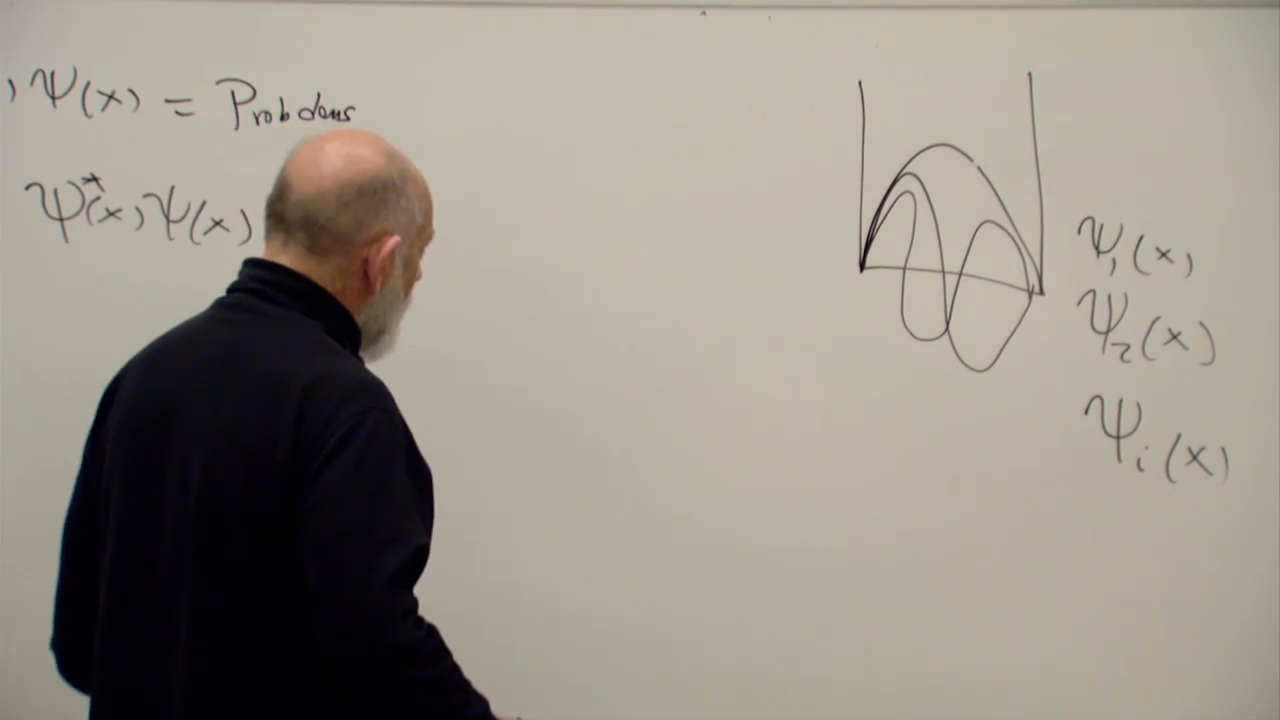
\includegraphics[width=0.94\linewidth]{lecture_07_frame_01.png}
\caption{Моды в ящике на лекционной доске. Следы слева — это одночастичная плотность Борна и нормировка; яма справа показывает \(\psi_1(x)\), \(\psi_2(x)\) и общее обозначение \(\psi_i(x)\).}
\lectureframe{00:08:25}
\end{figure}

Ту же структуру мод можно отделить от перекрытия на кадре с доски:
\begin{figure}[htbp]
\centering
\begin{tikzpicture}[x=1cm,y=1cm]
  \draw[thick] (0,0) -- (0,4.0);
  \draw[thick] (7,0) -- (7,4.0);
  \draw[gray!55] (0,2.85) -- (7,2.85);
  \draw[gray!55] (0,1.35) -- (7,1.35);
  \draw[blue!75!black,thick,domain=0:7,samples=120]
    plot (\x,{2.85+0.62*sin(180*\x/7)});
  \draw[teal!70!black,thick,domain=0:7,samples=120]
    plot (\x,{1.35+0.55*sin(360*\x/7)});
  \node[right] at (7.15,3.20) {$\psi_1(x)$};
  \node[right] at (7.15,1.70) {$\psi_2(x)$};
  \node at (3.5,0.38) {$\vdots\quad\psi_i(x)$};
\end{tikzpicture}
\caption{Чистая реконструкция качественного эскиза ящика. Вертикальные смещения лишь разделяют две волновые функции для наглядности.}
\end{figure}

Ортонормированность выражается равенством
\begin{equation}
\int dx\,\psi_i^*(x)\psi_j(x)=\delta_{ij}.
\label{eq:l07-orthonormality}
\end{equation}
Если \(i=j\), состояние нормировано и интеграл равен единице. Если \(i\ne j\), два состояния ортогональны и интеграл обращается в нуль.

Полнота — столь же важное утверждение
\begin{equation}
\sum_i |i\rangle\langle i|=\mathbf 1.
\label{eq:l07-resolution}
\end{equation}
Каждый оператор \(|i\rangle\langle i|\) проектирует на одно направление базиса; сумма по полному базису дает единичный оператор. Действуя на произвольный вектор, она просто разлагает этот вектор на компоненты и снова собирает его.

Теперь вставим равенство~\eqref{eq:l07-resolution} между двумя состояниями положения:
\begin{align}
\langle y|x\rangle
&=\sum_i\langle y|i\rangle\langle i|x\rangle \\
&=\sum_i\psi_i(y)\psi_i^*(x) \\
&=\delta(y-x).
\label{eq:l07-position-completeness}
\end{align}
Звездочка должна стоять у того множителя, чей порядок бра и кет равен \(\langle i|x\rangle\). Перестановка \(x\) и \(y\) дает комплексно-сопряженную, но эквивалентную форму. Таким образом, всякий полный ортонормированный базис задает представление дельта-функции. Синусы, косинусы, волновые функции осциллятора и собственные функции энергии выполняют одну и ту же роль.

\begin{classroomqa}
\lecturetimestamp{00:13:43}
\audiencequestion{Должна ли вторая волновая функция в сумме полноты стоять с комплексным сопряжением?}
\lecturerresponse{Да. При порядке \(\langle y|i\rangle\langle i|x\rangle\) множители равны \(\psi_i(y)\psi_i^*(x)\). Если держать порядок бра и кет на виду, звездочку не придется угадывать или ставить не туда.}
\end{classroomqa}

Это вся одночастичная математика, которая нам понадобится. Теперь мы меняем пространство состояний.

\section{Пространство Фока как более широкое пространство состояний}

Для многих тождественных частиц удобный базис фиксирует, сколько частиц занимает каждую одночастичную моду:
\begin{equation}
|n_1,n_2,n_3,\ldots\rangle.
\label{eq:l07-fock-basis}
\end{equation}
Целое число \(n_i\) есть число заполнения моды \(i\). Этот кет — не одночастичное состояние, записанное в необычной нотации. Он принадлежит большему гильбертову пространству, содержащему сектор с нулем частиц, все одночастичные состояния, все двухчастичные состояния и так далее. Это большее пространство называется пространством Фока.

Чтобы изменять заполнения, введем для каждой моды оператор рождения и оператор уничтожения,
\begin{equation}
a_i^\dagger,\qquad a_i.
\end{equation}
Первый добавляет одну частицу в моду \(i\), а второй убирает одну. На этом этапе язык гармонического осциллятора служит средством учета: здесь не обязательно буквально колеблется пружина. Алгебра осциллятора дает нам в точности тот аппарат, который нужен для повышения и понижения чисел заполнения.

Оператор числа заполнения моды имеет вид
\begin{equation}
\begin{aligned}
N_i&=a_i^\dagger a_i,\\
N_i|n_1,\ldots,n_i,\ldots\rangle
&=n_i|n_1,\ldots,n_i,\ldots\rangle.
\end{aligned}
\end{equation}
Вакуум есть
\begin{equation}
|0\rangle\equiv|0,0,0,\ldots\rangle,
\qquad
a_i|0\rangle=0
\quad\text{for every }i.
\label{eq:l07-vacuum}
\end{equation}
Поэтому одночастичное состояние в моде \(i\) равно
\begin{equation}
|i\rangle=a_i^\dagger|0\rangle.
\label{eq:l07-mode-created}
\end{equation}
Один и тот же символ \(|i\rangle\) теперь можно понимать либо как базисный вектор одночастичного пространства, либо как тот же вектор, вложенный в одночастичный сектор пространства Фока. Это вложение задается уравнением~\eqref{eq:l07-mode-created}; из окружающего контекста ясно, о каком пространстве идет речь.

\section{Объединение мод в поле}

Определим поля уничтожения и рождения как
\begin{equation}
\Psi(x)=\sum_i \psi_i(x)a_i,
\qquad
\Psi^\dagger(x)=\sum_i \psi_i^*(x)a_i^\dagger.
\label{eq:l07-field-expansion}
\end{equation}
Заглавная буква здесь существенна. Функции со строчной буквой \(\psi_i(x)\) — это комплексные числа; заглавная \(\Psi(x)\) есть оператор в пространстве Фока. В каждой пространственной точке \(x\) уравнение~\eqref{eq:l07-field-expansion} задает другую линейную комбинацию операторов мод. Именно это и означает операторнозначная функция положения.

Для свободных частиц функциями мод могут служить плоские волны \(e^{ikx}\). Тогда уравнение~\eqref{eq:l07-field-expansion} представляет собой разложение Фурье, за исключением того, что его коэффициенты Фурье — операторы, а не числа. В старой терминологии обычные комплексные числа называются \(c\)-числами, а квантовые операторы — \(q\)-числами. Функции мод являются \(c\)-числами и коммутируют со всем; операторный характер несут \(a_i\) и \(a_i^\dagger\).

Ни \(\Psi\), ни \(\Psi^\dagger\) не являются эрмитовыми. Они взаимно сопряжены. Две комбинации
\begin{equation}
\Psi+\Psi^\dagger,
\qquad
i(\Psi^\dagger-\Psi)
\label{eq:l07-hermitian-combinations}
\end{equation}
эрмитовы и могут представлять наблюдаемые. Однако пока поля наиболее полезны как средства, которые локально рождают, уничтожают и считают частицы.

\begin{classroomqa}
\lecturetimestamp{00:21:05}
\audiencequestion{Что означает, что оператор зависит от \(x\)?}
\lecturerresponse{Это означает, что каждому значению \(x\) соответствует свой оператор. Пространственная зависимость содержится в обычных функциях мод, тогда как каждая получающаяся линейная комбинация действует в одном и том же пространстве Фока.}
\end{classroomqa}

\section{Что делает поле рождения}

Определение становится полезным, когда мы спрашиваем, что оно делает. Начнем с собственного состояния положения в одночастичном секторе и вставим разложение единицы:
\begin{align}
|x\rangle
&=\sum_i |i\rangle\langle i|x\rangle \\
&=\sum_i a_i^\dagger|0\rangle\,\psi_i^*(x) \\
&=\Psi^\dagger(x)|0\rangle.
\label{eq:l07-local-creation}
\end{align}
Таким образом, \(a_i^\dagger\) рождает частицу в определенной моде \(i\), тогда как \(\Psi^\dagger(x)\) рождает частицу, локализованную в точке \(x\). В идеализированном базисе положений такая локализация понимается в смысле распределений; при физическом приготовлении использовался бы узкий волновой пакет, но алгебраический смысл остается тем же.

\begin{classroomqa}
\lecturetimestamp{00:24:48}
\audiencequestion{Является ли \(\sum_i|i\rangle\langle i|\) проектором?}
\lecturerresponse{Каждое слагаемое есть проектор на одно базисное состояние. Полная сумма есть сама единица и называется разложением единицы. Ее вставка не меняет никакого состояния, но выявляет компоненты состояния в выбранном базисе.}
\end{classroomqa}

Уравнение~\eqref{eq:l07-local-creation} дает первое прямое истолкование поля в терминах частиц. Мы не просто прикрепили пространственную метку к абстрактному оператору. Мы построили операцию, создающую частицу в этой пространственной точке.

\begin{classroomqa}
\lecturetimestamp{00:28:20}
\audiencequestion{Следует ли помечать поле рождения в координатном представлении звездочкой или даггером?}
\lecturerresponse{Для сопряжения оператора используйте даггер. Звездочки обозначают комплексное сопряжение обычных волновых функций \(\psi_i(x)\); даггер должен стоять у \(a_i^\dagger\) и \(\Psi^\dagger(x)\).}
\end{classroomqa}

\begin{classroomqa}
\lecturetimestamp{00:28:36}
\audiencequestion{Можно ли в разложении по модам переставлять операторы рождения через волновые функции?}
\lecturerresponse{Да. \(\psi_i(x)\) — \(c\)-числа, поэтому они коммутируют с любым оператором. Осторожность нужна только при изменении порядка некоммутирующих операторов, таких как \(a_i\) и \(a_j^\dagger\).}
\end{classroomqa}

\section{От плотности вероятности к плотности частиц}

Теперь немного поиграем с полем. Первое естественное выражение таково:
\begin{equation}
\int dx\,\Psi^\dagger(x)\Psi(x).
\end{equation}
Оно похоже на одночастичный нормировочный интеграл, но теперь его множители — операторы. Подставим разложения по модам, не меняя их порядка:
\begin{align}
\int dx\,\Psi^\dagger(x)\Psi(x)
&=\int dx
\left(\sum_i a_i^\dagger\psi_i^*(x)\right)\\
&\qquad\times\left(\sum_j a_j\psi_j(x)\right) \\
&=\sum_{i,j}a_i^\dagger a_j
\int dx\,\psi_i^*(x)\psi_j(x) \\
&=\sum_{i,j}a_i^\dagger a_j\,\delta_{ij} \\
&=\sum_i a_i^\dagger a_i.
\label{eq:l07-number-derivation}
\end{align}
Следовательно, оператор полного числа частиц равен
\begin{equation}
N=\sum_i N_i
=\int dx\,\Psi^\dagger(x)\Psi(x).
\label{eq:l07-total-number}
\end{equation}
Для обсуждаемых состояний возбуждения с конечной энергией числа заполнения убывают при достаточно большой энергии моды, так что эта сумма обычно конечна, хотя список возможных мод бесконечен.

Подынтегральное выражение — это оператор локальной плотности частиц:
\begin{equation}
n(x)=\Psi^\dagger(x)\Psi(x).
\label{eq:l07-density}
\end{equation}
Строго говоря, плотность в математической точке не измеряют. Для малой области \(R\) измеряют
\begin{equation}
N_R=\int_R dx\,n(x),
\label{eq:l07-regional-number}
\end{equation}
число частиц в этой области. Как и любая квантовая наблюдаемая, \(N_R\) не обязано иметь определённое значение в произвольном состоянии. Повторные приготовления могут давать разные результаты.

\begin{classroomqa}
\lecturetimestamp{00:36:27}
\audiencequestion{Является ли \(\Psi^\dagger(x)\Psi(x)\) многочастичной плотностью вероятности?}
\lecturerresponse{Его прямой смысл — плотность частиц. Многочастичная амплитуда вероятности, вообще говоря, зависит от координат всех частиц. Напротив, локальная билинейная комбинация при интегрировании по этой области подсчитывает число частиц в ней.}
\end{classroomqa}

\begin{classroomqa}
\lecturetimestamp{00:38:28}
\audiencequestion{Действуют ли операторы \(a_i\) и \(a_i^\dagger\) только на векторы состояния, а не на одночастичные волновые функции?}
\lecturerresponse{Да. Они действуют на состояния пространства Фока, такие как \(|n_1,n_2,\ldots\rangle\). Одночастичные модовые функции, которыми они умножаются, — обычные числа и не являются теми объектами, на которые действуют эти лестничные операторы.}
\end{classroomqa}

Кеты чисел заполнения образуют базис, а не наиболее общее состояние. Из них можно строить суперпозиции, в том числе такие, в которых одно и то же полное число по-разному распределено по модам. Для нейтральных частиц, таких как фотоны, можно также суперпонировать разные полные числа частиц. Оператор в уравнении~\eqref{eq:l07-regional-number} сохраняет один и тот же операциональный смысл во всех таких состояниях.

\begin{classroomqa}
\lecturetimestamp{00:40:01}
\audiencequestion{Если разделить плотность частиц на полное число, станет ли она плотностью вероятности обнаружить частицу в \(x\)?}
\lecturerresponse{При фиксированном \(N\) и большом числе частиц \(N_R/N\) является относительной частотой и обычно очень хорошо соответствует одночастичной вероятности. Это не операторное тождество, отождествляющее результат одного измерения с вероятностью. Измеренное число флуктуирует, обычно на величину порядка \(\sqrt N\) в картине независимых частиц, и в отдельной исключительной реализации оно может сильно отличаться от вероятности, хотя такая реализация маловероятна.}
\end{classroomqa}

\begin{classroomqa}
\lecturetimestamp{00:42:25}
\audiencequestion{Что происходит с сохранением заряда в суперпозиции одноэлектронного состояния и состояния без электронов?}
\lecturerresponse{Это не тот вид суперпозиции, который используют для замкнутого сектора с фиксированным электрическим зарядом. Можно суперпонировать разные распределения с одним и тем же полным зарядом. Фотоны не несут электрического заряда, поэтому разные секторы с различным числом фотонов такой проблемы не создают. Числа электронов и позитронов также могут изменяться совместно, тогда как суммарный заряд остаётся фиксированным.}
\end{classroomqa}

\section{Энергия независимых частиц}

Следующая наблюдаемая — энергия. Сначала ограничимся частицами, которые не взаимодействуют друг с другом. В разреженной системе это часто хорошее приближение. Даже фотоны в принципе взаимодействуют через процессы более высокого порядка, но обычное лабораторное излучение достаточно разрежено, так что описание независимыми частицами превосходно.

Пусть \(\omega_i\) обозначает энергию одной частицы в моде \(i\), при \(\hbar=1\). Под модой здесь понимается одно одночастичное состояние. Тогда полный гамильтониан имеет вид
\begin{equation}
H=\sum_i\omega_i N_i
=\sum_i\omega_i a_i^\dagger a_i.
\label{eq:l07-mode-hamiltonian}
\end{equation}
Каждая занятая мода вносит свою одночастичную энергию по одному разу на каждую частицу.

\begin{classroomqa}
\lecturetimestamp{00:48:16}
\audiencequestion{Является ли \(\omega_i\) функцией положения?}
\lecturerresponse{Нет. Это собственное значение энергии, связанное с модой \(i\). Функция \(\psi_i(x)\) зависит от положения; \(\omega_i\) зависит от того, какой энергетический уровень выбран.}
\end{classroomqa}

Значения \(\omega_i\) определяются стационарным одночастичным уравнением Шрёдингера. Определим
\begin{equation}
h=-\frac{\nabla^2}{2m}+V(x).
\label{eq:l07-one-particle-h}
\end{equation}
Тогда
\begin{equation}
h\psi_i(x)=\omega_i\psi_i(x).
\label{eq:l07-schrodinger-eigenvalue}
\end{equation}
В одном измерении оператор импульса равен \(p=-i\partial_x\), и \(p^2/(2m)\) принимает вид \(-\partial_x^2/(2m)\). В трёх измерениях три вторые производные объединяются в \(-\nabla^2/(2m)\).

\begin{figure}[htbp]
\centering
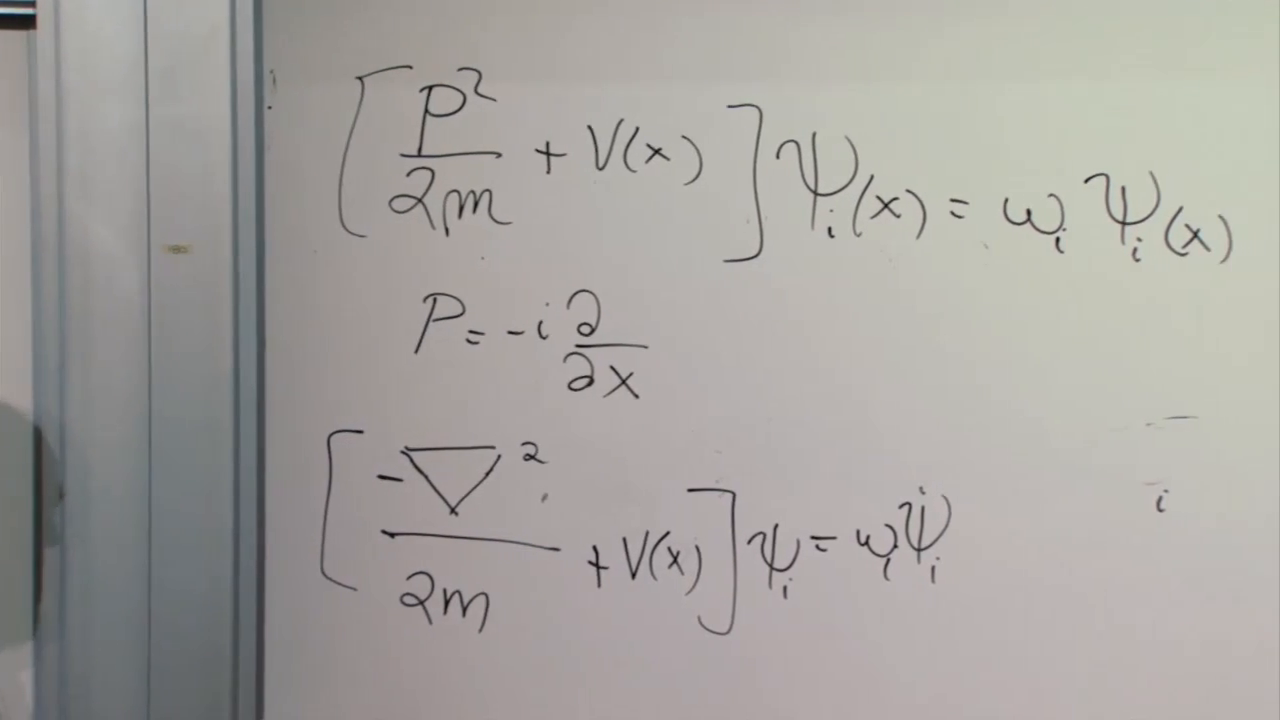
\includegraphics[width=0.94\linewidth]{lecture_07_frame_02.png}
\caption{Переход на доске от \(p^2/(2m)+V(x)\) к дифференциальной форме одночастичного уравнения Шрёдингера на собственные значения. В ~\eqref{eq:l07-schrodinger-eigenvalue} приведена его аккуратно восстановленная запись.}
\lectureframe{00:54:10}
\end{figure}

Для произвольной нормированной одночастичной волновой функции знакомое среднее значение имеет вид
\begin{equation}
\langle h\rangle_\psi
=\int dx\,\psi^*(x)h\psi(x).
\label{eq:l07-one-particle-energy-expectation}
\end{equation}
Многочастичная формула напрашивается, если заменить волновую функцию со строчной буквой операторнозначным полем. Это ещё не доказательство; это догадка, правильность которой мы сейчас проверим:
\begin{equation}
H=\int dx\,\Psi^\dagger(x)h\Psi(x).
\label{eq:l07-field-hamiltonian}
\end{equation}

\section{Сначала ответ, затем доказательство}

Подставим ~\eqref{eq:l07-field-expansion} в предложенный гамильтониан:
\begin{align}
\int dx\,\Psi^\dagger h\Psi
&=\int dx
\left(\sum_i a_i^\dagger\psi_i^*(x)\right)
h\left(\sum_j a_j\psi_j(x)\right) \\
&=\sum_{i,j}a_i^\dagger a_j
\int dx\,\psi_i^*(x)h\psi_j(x).
\label{eq:l07-h-expanded}
\end{align}
Дифференциальный оператор \(h\) действует на зависящую от \(x\) волновую функцию \(\psi_j(x)\), а не на оператор моды \(a_j\). Согласно уравнению Шрёдингера,
\begin{equation}
h\psi_j(x)=\omega_j\psi_j(x).
\end{equation}
Следовательно,
\begin{align}
\int dx\,\Psi^\dagger h\Psi
&=\sum_{i,j}a_i^\dagger a_j\omega_j
\int dx\,\psi_i^*(x)\psi_j(x) \\
&=\sum_{i,j}a_i^\dagger a_j\omega_j\delta_{ij} \\
&=\sum_j\omega_j a_j^\dagger a_j.
\label{eq:l07-h-proof}
\end{align}
Это в точности уравнение~\eqref{eq:l07-mode-hamiltonian}. Локальное полевое выражение и сумма энергий всех частиц — один и тот же оператор.

\begin{figure}[htbp]
\centering
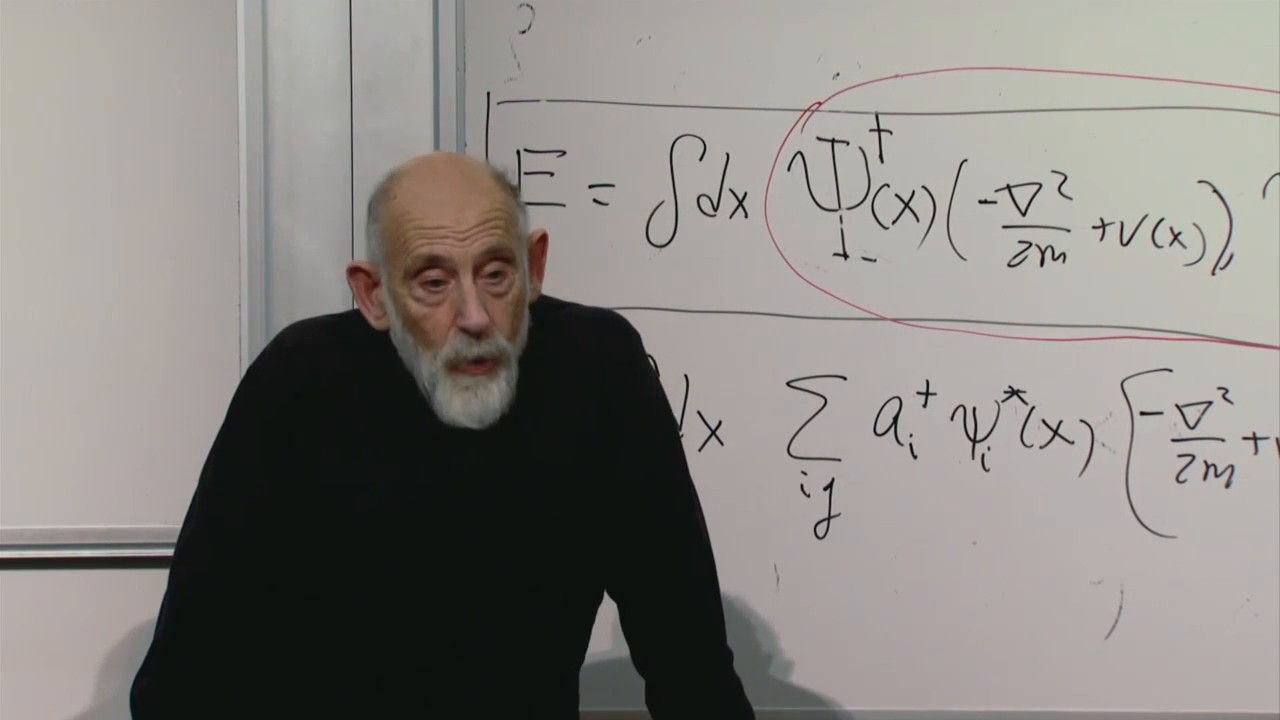
\includegraphics[width=0.94\linewidth]{lecture_07_frame_03.png}
\caption{Полевой гамильтониан, выделенный на доске, а под ним — начало доказательства через разложение по модам. Кадр лекции сохранён как свидетельство; уравнения~\eqref{eq:l07-field-hamiltonian}--\eqref{eq:l07-h-proof} восстанавливают полную алгебру.}
\lectureframe{01:05:34}
\end{figure}

В этом выводе ни один оператор рождения не переставлялся через оператор уничтожения. Порядок \(a_i^\dagger a_j\) сохраняется от начала до конца. Свободно перемещаются только волновые функции, являющиеся \(c\)-числами, и соответствующие им собственные значения.

\section{Почему это поле}

Почему \(\Psi(x)\) называют полем? Потому что это операторнозначная величина, определённая в каждой точке пространства, а эрмитовы комбинации или билинейные выражения, построенные из неё, являются локальными наблюдаемыми. Плотность \(n(x)\) и приведённое ниже локальное выражение для энергии — два примера. За этим словом не скрывается никакого дополнительного математического критерия.

Это поле — не электромагнитное поле. Оно описывает тот нерелятивистский вид частиц, который задаёт одночастичные моды и гамильтониан \(p^2/(2m)+V\): например, медленно движущиеся атомы, нейтроны, протоны или электроны. Эти частицы являются квантами соответствующего поля в том же структурном смысле, в каком фотоны являются квантами электромагнитного поля.

\begin{classroomqa}
\lecturetimestamp{01:02:45}
\audiencequestion{Где при переходе от многочастичной системы к приведённой выше формуле появилось поле?}
\lecturerresponse{Оно появляется в уравнении~\eqref{eq:l07-field-expansion}: \(\Psi(x)\) — оператор в каждой точке пространства. Последующие выводы показывают, что его локальные произведения измеряют плотности частиц и энергии. Зависимость от положения вместе с операторным содержанием и образует именно ту полевую структуру, которая здесь строится.}
\end{classroomqa}

\section{Локальная плотность энергии}

В ~\eqref{eq:l07-field-hamiltonian} полная энергия записывается как интеграл по пространству,
\begin{equation}
\begin{aligned}
H&=\int dx\,\mathcal H(x),\\
\mathcal H(x)
&=-\frac{1}{2m}\Psi^\dagger(x)\nabla^2\Psi(x)\\
&\quad+V(x)\Psi^\dagger(x)\Psi(x).
\end{aligned}
\label{eq:l07-hamiltonian-density}
\end{equation}
Подынтегральное выражение — естественная локальная плотность энергии для этого гамильтониана. Её локальная форма не единственна. Например, интегрирование по частям заменяет кинетический член на
\begin{equation}
\mathcal H_{\rm kin}(x)
=\frac{1}{2m}\nabla\Psi^\dagger(x)\mathbin{\cdot}\nabla\Psi(x)
\label{eq:l07-kinetic-density}
\end{equation}
с точностью до граничного члена. Оба выражения дают один и тот же полный гамильтониан при обычных граничных условиях. Это и есть та небольшая неоднозначность, о которой говорилось на лекции.

\begin{classroomqa}
\lecturetimestamp{01:05:57}
\audiencequestion{Нужно ли интегрировать плотность энергии по всему пространству?}
\lecturerresponse{Интегрирование по всему пространству даёт полную энергию. Интегрирование по меньшей области даёт энергию, приписываемую этой области, с обычной неоднозначностью выбора локальной плотности, полный интеграл от которой даёт тот же гамильтониан.}
\end{classroomqa}

\begin{classroomqa}
\lecturetimestamp{01:06:25}
\audiencequestion{Чем заглавное \(N_i\) в формуле для энергии отличается от строчного \(n_i\)?}
\lecturerresponse{\(N_i=a_i^\dagger a_i\) — оператор. Целое число \(n_i\) является одним из его собственных значений на состоянии с заданными числами заполнения. Операторы действуют на состояния; их собственные значения — обычные числа.}
\end{classroomqa}

\begin{classroomqa}
\lecturetimestamp{01:06:46}
\audiencequestion{Можно ли сам гамильтониан поля записать в нотации Дирака как бра или кет?}
\lecturerresponse{Нет. Бра и кеты обозначают векторы состояний и двойственные к ним векторы. Поле и гамильтониан — это операторы, действующие на эти состояния. В выражении для среднего значения, таком как \(\langle\Phi|H|\Phi\rangle\), используются оба типа объектов, и отождествлять их нельзя.}
\end{classroomqa}

\section{Восстановление одночастичного случая и приближение к классическому полю}

Расширенный формализм содержит обычную одночастичную квантовую механику. Ограничим пространство Фока состояниями, для которых выполняется
\begin{equation}
N|\Phi\rangle=|\Phi\rangle.
\end{equation}
Внутри этого сектора полевая конструкция воспроизводит любое одночастичное состояние и любое одночастичное предсказание. Мы не заменили старую теорию; мы вложили её в пространство, которое может также описывать 0, 2 или сколь угодно много частиц.

На другом пределе мода, занятая очень большим числом бозонов, может приближённо вести себя как классическая волна. В подходящих когерентных или полуклассических состояниях среднее значение
\begin{equation}
\Phi_{\rm cl}(x,t)=\langle\Psi(x,t)\rangle
\end{equation}
удовлетворяет имеющему классический вид уравнению
\begin{equation}
i\partial_t\Phi_{\rm cl}(x,t)
=\left(-\frac{\nabla^2}{2m}+V(x)\right)\Phi_{\rm cl}(x,t)
\label{eq:l07-classical-schrodinger}
\end{equation}
для свободной нерелятивистской теории. В лекции эта связь констатируется, а не выводится. Это мост между совокупностью квантов и волновым полем: большие числа заполнения подавляют относительные флуктуации и заставляют подходящие средние значения вести себя классически.

Следовательно, этот формализм служит и для учёта, и для описания физики. Он организует все секторы с различным числом частиц, но также охватывает интерференцию, запутанность и возникновение классических волн из квантовых частиц.

\begin{classroomqa}
\lecturetimestamp{01:10:43}
\audiencequestion{Почему под интегралом с операторами рождения и уничтожения можно обращаться почти так, как если бы это были обычные числа?}
\lecturerresponse{Их между собой не переставляли. Обычные модовые функции коммутируют с ними, а производные действуют только на эти функции. Чтобы провести оператор уничтожения сквозь оператор рождения, понадобился бы коммутатор, и мог бы добавиться дополнительный член; в доказательстве такого шага нет.}
\end{classroomqa}

\section{Отступление о нотации Дирака}

Часть путаницы носит исторический характер. Одночастичная волновая функция удовлетворяет волновому уравнению и внешне похожа на классическое поле, но при этом она также является амплитудой вероятности. Ранняя квантовая теория должна была разделить эти роли, а затем объяснить, как действительно измеримые волновые поля, такие как электромагнетизм, состоят из квантов. Пространство Фока и операторнозначные поля снимают это кажущееся противоречие.

Нотация Дирака делает это разграничение необычайно компактным. Кет принадлежит векторному пространству, бра — его двойственному пространству, а их запись рядом образует скалярное произведение. Тогда разложение единицы
\begin{equation}
\sum_i|i\rangle\langle i|=\mathbf 1
\end{equation}
становится почти самоочевидным. Лекция иллюстрирует это анекдотом из преподавания квантовой механики математикам: математическое содержание уже было знакомо, но нотация делала рутинные преобразования настолько прозрачными, что структура казалась новой. Смысл не в том, что в одной дисциплине не было соответствующего понятия. Дело в том, что удачно выбранная нотация сильно затрудняет путаницу в допустимых операциях.

Этот урок важен и здесь. Теперь есть несколько различных операторов:
\begin{itemize}
\item \(h\) действует на одночастичные волновые функции как дифференциальный оператор;
\item \(a_i\) и \(a_i^\dagger\) действуют на состояния с числами заполнения в пространстве Фока;
\item \(\Psi(x)\), \(\Psi^\dagger(x)\), \(N\) и \(H\) также действуют на пространство Фока.
\end{itemize}
Разложение в уравнении~\eqref{eq:l07-field-expansion} связывает первые два описания, не сливая их.

\begin{classroomqa}
\lecturetimestamp{01:18:16}
\audiencequestion{Являются ли поля лишь формализмом для описания совокупностей частиц?}
\lecturerresponse{Это формализм, но не пустой. Их локальные наблюдаемые можно измерять, а частицы здесь квантовые, с интерференцией и запутанностью, а не классические шарики. Полевые операторы кодируют именно эти измеримые коллективные свойства.}
\end{classroomqa}

\section{Релятивистская оговорка и электромагнитное отступление}

Построение до сих пор было нерелятивистским. Импульс остаётся хорошей меткой частицы и в релятивистской физике, но резко локализованное положение частицы — гораздо более тонкое понятие. Поэтому локальная плотность числа фотонов, вообще говоря, не является столь же чистым объектом, как нерелятивистское \(n(x)\). Плотность энергии остаётся хорошо определённой и является более надёжной локальной наблюдаемой.

Лекция приводит полезную, явно эвристическую электромагнитную аналогию. Объединим электрическое и магнитное поля в комплексный вектор
\begin{equation}
\mathbf F=\mathbf E+i\mathbf B,
\qquad
\mathbf F^*=\mathbf E-i\mathbf B.
\label{eq:l07-riemann-silberstein}
\end{equation}
Тогда
\begin{equation}
\mathbf F^*\mathbin{\cdot}\mathbf F
=\mathbf E^2+\mathbf B^2,
\label{eq:l07-em-density}
\end{equation}
что в обычных единицах пропорционально плотности электромагнитной энергии. Это не является в буквальном смысле плотностью вероятности фотона. Лучше рассматривать это как компактную полевую переменную, квадрат модуля которой измеряет плотность энергии, или, неформально, как плотность фотонов, взвешенную по энергии фотона.

\begin{classroomqa}
\lecturetimestamp{01:19:10}
\audiencequestion{Можно ли отождествить плотность фотонов с напряжённостью электрического поля?}
\lecturerresponse{Лишь качественно и с осторожностью. Для релятивистских фотонов локальное число частиц не является предпочтительным понятием. Надёжное утверждение состоит в том, что \(E^2+B^2\) пропорционально плотности энергии, а комплексная комбинация \(\mathbf E+i\mathbf B\) позволяет компактно записать уравнения Максвелла в шрёдингероподобной форме.}
\end{classroomqa}

\begin{classroomqa}
\lecturetimestamp{01:20:09}
\audiencequestion{Почему релятивистская частица может иметь определённый импульс, тогда как положение проблематично?}
\lecturerresponse{Импульс служит чистой меткой релятивистских одночастичных представлений, тогда как строгая локализация конфликтует с рождением частиц и релятивистским полевым описанием. В этой лекции эта теория не развивается; предупреждение лишь отмечает предел нынешней нерелятивистской интерпретации плотности.}
\end{classroomqa}

\section{Упорядочение и постоянная основного состояния}

Порядок операторов нельзя менять небрежно. Для бозонных мод
\begin{equation}
a_i a_i^\dagger=a_i^\dagger a_i+1.
\end{equation}
Соответственно, замена нормального порядка \(\Psi^\dagger h\Psi\) на обратный порядок \((h\Psi)\Psi^\dagger\), или на его надлежащим образом проинтегрированный аналог, добавляет вклад коммутатора. В модовом базисе это даёт аддитивную сумму по одному кванту энергии на каждую моду. Это постоянная основного состояния, или константа нулевых колебаний, и в континууме она требует регуляризации. Лекция не разбирает здесь этот вопрос; она лишь предупреждает, что эти два упорядочения не равны.

\begin{classroomqa}
\lecturetimestamp{01:22:04}
\audiencequestion{Что происходит, если \(\Psi\) и \(\Psi^\dagger\) переставить местами в гамильтониане?}
\lecturerresponse{Нужно учесть их коммутатор. Поэтому обращение порядка добавляет не зависящий от состояния вклад основного состояния, а не воспроизводит то же самое выражение. Выписанный гамильтониан оставлен в нормальном порядке, \(\Psi^\dagger h\Psi\).}
\end{classroomqa}

\section{Импульс как последняя проверка}

В последние минуты ещё раз повторяется тот же самый переход к оператору. Для одной частицы
\begin{equation}
\langle p\rangle_\psi
=\int dx\,\psi^*(x)\left(-i\partial_x\right)\psi(x).
\label{eq:l07-one-particle-momentum}
\end{equation}
Если заменить волновую функцию полем, получим оператор полного импульса
\begin{equation}
P=\int dx\,\Psi^\dagger(x)\left(-i\partial_x\right)\Psi(x),
\label{eq:l07-field-momentum}
\end{equation}
или, в трёх измерениях,
\begin{equation}
\mathbf P=\int d^3x\,\Psi^\dagger(\mathbf x)
\left(-i\boldsymbol\nabla\right)\Psi(\mathbf x).
\end{equation}
Поля несут импульс. Достаточно мощный лазер передаёт импульс стенке и оказывает силу; в квантовом описании этот импульс поля есть сумма импульсов фотонов.

Формула~\eqref{eq:l07-field-momentum} — это оператор, а не среднее значение. Для состояния пространства Фока \(|\Phi\rangle\) можно затем вычислить
\begin{equation}
\langle P\rangle_\Phi=\langle\Phi|P|\Phi\rangle.
\end{equation}
И оператор, и состояние необходимы для образования среднего значения. Путать наблюдаемую с её средним значением значило бы стереть именно то различие, которое лекция старалась установить.

\begin{classroomqa}
\lecturetimestamp{01:26:02}
\audiencequestion{Является ли выписанный импульс поля уже средним импульсом?}
\lecturerresponse{Нет. Это эрмитов оператор, представляющий наблюдаемую. Задайте состояние и заключите оператор между его бра и кетом, чтобы получить среднее значение; измерение всё же может флуктуировать вокруг этого среднего.}
\end{classroomqa}

На этом естественно остановиться. Исходя из частиц, мы построили локальные поля рождения и уничтожения, использовали их для подсчёта частиц и переписали сумму одночастичных энергий и импульсов в виде полевых операторов. Следующий шаг — не очередная смена обозначений. Он состоит в том, чтобы полевые операторы представляли физические процессы: распад частиц, рассеяние частиц и превращение одних видов частиц в другие.

\chapter{Смешивание, осцилляции, электрические дипольные моменты и полевые операторы}

Начнём немного в стороне от заявленной темы — с вопроса о нейтрино. Имеются свидетельства того, что нейтрино обладают массой и что типы нейтрино смешиваются. Если массы не у всех одинаковы, как один тип может превращаться в другой, не нарушая закон сохранения энергии?

Этот вопрос указывает на общую схему, встречающуюся повсюду в квантовой механике: состояния, в которых систему подготавливают или регистрируют, не обязаны быть состояниями, диагонализующими её гамильтониан. Состояние с определённой энергией лишь приобретает фазу. Подготовленное состояние, являющееся суперпозицией нескольких энергий, изменяется потому, что его компоненты приобретают разные фазы. Именно это различие проведёт нас от двухъямного потенциала к нейтринным осцилляциям и прецессии спина. После отступления об электрическом дипольном моменте электрона мы вернёмся ко вторичному квантованию и увидим на уровне операторов ту же координатно--импульсную фурье-структуру.

\section{Смешивание как суть вопроса}

Масса у всех нейтрино не обязана быть одинаковой. Собственные состояния энергии не смешиваются друг с другом; каждое эволюционирует независимо. То, что мы называем \emph{типом}, или ароматом, нейтрино, связано с тем, как оно рождается и регистрируется, и состояние с определённым ароматом может быть линейной комбинацией собственных состояний массы и энергии. Схематически,
\begin{equation}
|\text{type}\rangle = \sum_n c_n |E_n\rangle .
\end{equation}
Следовательно, правильно говорить не о том, что собственные состояния энергии переходят друг в друга, а о том, что состояния, называемые ``электронным нейтрино'' или ``мюонным нейтрино'', сами не обязаны быть собственными состояниями энергии.

\begin{classroomqa}
\lecturetimestamp{00:00:09}
\audiencequestion{Если массы нейтрино различны, как они могут смешиваться при сохранении энергии?}
\lecturerresponse{Собственные состояния массы и энергии не переходят друг в друга. Состояния электронного, мюонного и тау-аромата представляют собой различные линейные комбинации этих собственных состояний. Каждая массовая компонента эволюционирует со своей собственной фазой, и интерференция изменяет вероятности различных ароматов, не нарушая закона сохранения энергии.}
\end{classroomqa}

У этой структуры много примеров. Наиболее наглядный из них начинается с частицы в симметричном двухъямном потенциале.

\section{Симметричный двухъямный потенциал и приближённые локализованные состояния}

Рассмотрим частицу, движущуюся в симметричном двухъямном потенциале с высоким барьером между двумя минимумами. Если бы барьер был бесконечно высоким, левая и правая ямы были бы полностью развязаны. Можно было бы решать задачу для левой ямы так, как будто правой не существует, и аналогично для правой. Тогда приближёнными волновыми функциями основного состояния были бы локализованное слева состояние \(\psi_L\) и локализованное справа состояние \(\psi_R\), оба с одной и той же энергией \(E\).

В каждой изолированной яме основное состояние обладает привычными качественными свойствами: оно гладкое, не имеет узлов и находится при наименьшей возможной энергии, совместимой с локализацией. Представьте себе высокий центральный барьер как кирпичную стену. Рассматривать его как бесконечный — лишь приближение, но оно даёт нам полезную пару локализованных состояний, с которой можно начать.

\begin{figure}
\centering
\begin{adjustbox}{max width=\linewidth}
\begin{tikzpicture}[x=0.8cm,y=0.8cm]
\begin{scope}[shift={(-5.8,0)}]
\draw (-4,2.7) .. controls (-3.35,1.2) and (-2.55,-0.45) .. (-2.0,-0.72)
      .. controls (-1.35,-0.95) and (-0.7,0.65) .. (0,2.05)
      .. controls (0.7,0.65) and (1.35,-0.95) .. (2.0,-0.72)
      .. controls (2.55,-0.45) and (3.35,1.2) .. (4,2.7);
\draw[dashed] (-4,-0.10) -- (4,-0.10);
\node at (-3.55,-0.48) {$E$};
\draw[line width=0.9pt] (-4,-0.02) .. controls (-3.2,-0.02) and (-2.7,0.30) .. (-2.15,0.95)
      .. controls (-1.55,1.30) and (-1.15,0.35) .. (-0.55,-0.06)
      .. controls (0.15,-0.14) and (0.9,-0.15) .. (4,-0.15);
\node at (-2.15,1.35) {$\psi_L$};
\end{scope}
\begin{scope}[shift={(5.8,0)}]
\draw (-4,2.7) .. controls (-3.35,1.2) and (-2.55,-0.45) .. (-2.0,-0.72)
      .. controls (-1.35,-0.95) and (-0.7,0.65) .. (0,2.05)
      .. controls (0.7,0.65) and (1.35,-0.95) .. (2.0,-0.72)
      .. controls (2.55,-0.45) and (3.35,1.2) .. (4,2.7);
\draw[dashed] (-4,-0.10) -- (4,-0.10);
\node at (-3.55,-0.48) {$E$};
\draw[line width=0.9pt] (-4,-0.02) .. controls (-3.2,-0.01) and (-2.7,0.30) .. (-2.15,0.95)
      .. controls (-1.6,1.28) and (-1.1,0.25) .. (-0.30,-0.08)
      .. controls (0.35,-0.12) and (0.85,-0.12) .. (1.35,0.35)
      .. controls (1.9,0.88) and (2.35,1.15) .. (2.85,0.55)
      .. controls (3.2,0.05) and (3.55,-0.12) .. (4,-0.15);
\end{scope}
\end{tikzpicture}
\end{adjustbox}
\caption{Аккуратно перерисованный набросок с начальной доски. Слева показано одностороннее пробное состояние \(\psi_L\), полученное при предположении, что барьер фактически бесконечен. Справа та же волновая функция симметрично продолжена через барьер, что иллюстрирует малую, но ненулевую утечку, которая в конечном счёте приводит к истинному чётному основному состоянию.}
\end{figure}

С точки зрения квантовой механики, однако, барьер не является по-настоящему бесконечным. Волновая функция в области барьера не обращается точно в нуль; она лишь очень мала. Вся суть — в этой крошечной утечке. Именно она превращает лево-правое приближение в подлинную задачу о смешивании.

\section{Собственные состояния чётности и экспоненциальное расщепление уровней}

Теперь в эту локализованную картину вмешивается теорема: если потенциал симметричен, то точные собственные функции энергии можно выбрать либо симметричными, либо антисимметричными относительно отражения.

\begin{theorem}
Если \(V(x)=V(-x)\) в одном измерении, то собственные функции гамильтониана можно выбрать так, чтобы они удовлетворяли либо
\[
\psi(x)=\psi(-x)
\qquad \text{or} \qquad
\psi(x)=-\psi(-x).
\]
\end{theorem}

Теперь нужно внести поправку. Односторонние состояния \(\psi_L\) и \(\psi_R\) не являются ни симметричными, ни антисимметричными, поэтому они не могут быть точными собственными состояниями полного гамильтониана. Они являются хорошими приближёнными состояниями лишь тогда, когда барьер высок. Истинные собственные состояния — симметричная и антисимметричная комбинации,
\begin{align}
\psi_+ &= \frac{\psi_L+\psi_R}{\sqrt{2}},\\
\psi_- &= \frac{\psi_L-\psi_R}{\sqrt{2}}.
\end{align}
В обозначениях, которые и дальше останутся на доске, обозначим их энергии как
\begin{align}
H\psi_+ &= (E_1-\epsilon)\psi_+,\\
H\psi_- &= (E_1+\epsilon)\psi_-.
\end{align}
Тогда полное расщепление равно
\begin{equation}
\Delta E = (E_1+\epsilon)-(E_1-\epsilon)=2\epsilon .
\end{equation}

\begin{figure}[htbp]
\centering
\includegraphics[width=0.92\linewidth]{lecture_08_frame_02.png}
\caption{Волновая функция, симметрично продолженная в двухъямном потенциале. Её амплитуда под барьером мала, но не равна нулю, и именно это служит источником расщепления уровней.}
\lectureframe{00:06:19}
\end{figure}

\begin{figure}
\centering
\begin{tikzpicture}[x=1cm,y=1cm]
\draw[->] (0,0) -- (0,3);
\node[left] at (0,2.8) {energy};
\draw (-0.35,1.60) -- (0.35,1.60);
\node[left] at (-0.45,1.60) {$\psi_L,\psi_R$};
\node at (1.7,1.60) {$\Longrightarrow$};
\draw (3.0,1.32) -- (3.75,1.32);
\draw (3.0,1.88) -- (3.75,1.88);
\draw[dashed] (2.8,1.60) -- (3.95,1.60);
\node[right] at (3.9,1.32) {$\psi_+,\ E_1-\epsilon$};
\node[right] at (3.9,1.88) {$\psi_-,\ E_1+\epsilon$};
\node[below] at (3.37,1.60) {$E_1$};
\end{tikzpicture}
\caption{Логика туннельного расщепления, показанная на доске. Приближённые левые и правые состояния почти вырождены, но точные симметричное и антисимметричное собственные состояния расщеплены на малую величину \(2\epsilon\).}
\end{figure}

Упорядочение уровней и несёт физический смысл. Симметричное состояние имеет чуть меньшую энергию, потому что оно более гладко проходит через область барьера; то, что волновой функции позволено просачиваться и симметрично продолжаться, понижает энергию на крошечную величину. Антисимметричное состояние имеет чуть большую энергию, потому что первое возбуждённое состояние в одном измерении имеет один узел, и в этой симметричной задаче этот узел расположен в середине. Дополнительная кривизна увеличивает кинетическую энергию.

Эффект очень мал — экспоненциально мал по ширине и высоте барьера. Явная формула WKB нам здесь не нужна; важно, что расщепление реально, но мало. Помните также, что общий знак волновой функции не несёт физической информации. Замена \(\psi_-\) на \(-\psi_-\) не изменяет состояния.

\section{Эволюция во времени и лево-правые осцилляции}

Теперь зададим динамический вопрос: что происходит, если мы помещаем частицу в левую яму? Это решающий шаг, потому что осцилляция — это зависящее от времени проявление того же самого явления смешивания.

Обратные соотношения имеют вид
\begin{align}
\psi_L &= \frac{\psi_+ + \psi_-}{\sqrt{2}},\\
\psi_R &= \frac{\psi_+ - \psi_-}{\sqrt{2}}.
\end{align}
Поэтому первоначально локализованное слева состояние равно
\begin{equation}
\psi(0)=\psi_L=\frac{\psi_+ + \psi_-}{\sqrt{2}}.
\end{equation}
Это не собственное состояние энергии, и потому оно должно эволюционировать нетривиально.

Мы используем стандартное Schr\"odinger-соглашение \(e^{-iEt}\). Общая фаза не оказывает наблюдаемого эффекта; лишь относительная фаза между двумя энергетическими компонентами может переносить вероятность из одной ямы в другую.

С этим соглашением,
\begin{equation}
\psi(t)=\frac{1}{\sqrt{2}}\left(e^{-i(E_1-\epsilon)t}\psi_+ + e^{-i(E_1+\epsilon)t}\psi_-\right).
\end{equation}
Это приведённая в порядок версия формулы с доски. Теперь вынесем общую фазу:
\begin{equation}
\psi(t)=\frac{e^{-iE_1 t}}{\sqrt{2}}\left(e^{i\epsilon t}\psi_+ + e^{-i\epsilon t}\psi_-\right).
\end{equation}
Теперь одна фаза обходит единичную окружность в одну сторону, а другая — в противоположную. Состояние изменяется только потому, что эти две фазы постепенно расходятся по фазе.

Чтобы явно увидеть лево-правые осцилляции, подставим определения \(\psi_\pm\):
\begin{align}
\psi(t)
&= \frac{e^{-iE_1 t}}{2}
\left[e^{i\epsilon t}(\psi_L+\psi_R)+e^{-i\epsilon t}(\psi_L-\psi_R)\right] \\
&= \frac{e^{-iE_1 t}}{2}
\left[(e^{i\epsilon t}+e^{-i\epsilon t})\psi_L+(e^{i\epsilon t}-e^{-i\epsilon t})\psi_R\right] \\
&= e^{-iE_1 t}\left[\psi_L\cos(\epsilon t)+i\,\psi_R\sin(\epsilon t)\right].
\end{align}
Это ключевой подробно разобранный вывод этой главы. В двухсостояниевом приближении, где \(\psi_L\) и \(\psi_R\) ортонормированы, вероятности равны
\begin{equation}
P_L(t)=\cos^2(\epsilon t),
\qquad
P_R(t)=\sin^2(\epsilon t).
\end{equation}
Итак, система осциллирует. В промежуточные моменты времени она действительно находится в суперпозиции; например, при \(\epsilon t=\pi/4\) вероятности по обе стороны одинаковы. Фазы эволюционируют непрерывно, и локализация меняется непрерывно вместе с ними.

Вывод на доске выделяет первый момент времени, в который относительный знак меняется. Спрашивается, когда
\begin{equation}
e^{-i\epsilon t}=-\,e^{i\epsilon t},
\end{equation}
что и является заметной вехой на доске. После умножения получаем
\begin{equation}
e^{2i\epsilon t}=-1.
\end{equation}
При первом таком случае,
\begin{equation}
2\epsilon t=\pi,
\qquad\text{so}\qquad
t_{L\to R}=\frac{\pi}{2\epsilon}.
\end{equation}

\begin{figure}[htbp]
\centering
\includegraphics[width=0.94\linewidth]{lecture_08_frame_05.png}
\caption{Вычисление относительной фазы на доске. Две энергетические компоненты становятся противоположными при \(e^{2i\epsilon t}=-1\), что даёт первое время перехода \(2\epsilon t=\pi\). В набранном выводе используется одно последовательное Schr\"odinger-фазовое соглашение.}
\lectureframe{00:17:52}
\end{figure}
В этот момент,
\begin{equation}
\psi(t_{L\to R}) \propto \frac{\psi_+-\psi_-}{\sqrt{2}}=\psi_R.
\end{equation}
Общая фаза несущественна. Важно то, что частица, первоначально помещённая слева, эволюционировала в локализованное справа состояние. Ещё через такой же интервал она снова вернётся назад. Смешивание и осцилляция идут вместе.

Уравнение однозначно: малое \(\epsilon\) означает медленные осцилляции и длительное время перехода. Ни одно из локализованных состояний не имеет определённой энергии, но обе точные энергетические компоненты сохраняют энергию и эволюционируют в точности так, как должны.

\section{Аналогии с нейтрино, аммиаком и спином}

Двухъямный потенциал даёт нам схему для исходного вопроса о нейтрино. Нейтрино, рождённое вместе с электроном, называется электронным нейтрино; рождённое вместе с мюоном — мюонным нейтрино. Эти ароматовые метки описывают каналы рождения и регистрации. Состояния с определёнными массами и, следовательно, при фиксированном импульсе с определёнными энергиями свободной частицы образуют другой базис.

В простейшей схематичной двухсостоянийной модели с максимальным смешиванием,
\begin{equation}
|\nu_e\rangle \sim \frac{|m_1\rangle+|m_2\rangle}{\sqrt{2}},
\qquad
|\nu_\mu\rangle \sim \frac{|m_1\rangle-|m_2\rangle}{\sqrt{2}},
\end{equation}
где массовые собственные состояния играют роль \(\psi_+\) и \(\psi_-\), а состояния аромата играют роль \(\psi_L\) и \(\psi_R\). В реальном смешивании нейтрино вместо этих равных коэффициентов используется нетривиальная матрица смешивания, но сам механизм уже виден и здесь.

Нейтрино электронного аромата рождается в процессе с участием электрона, подобно тому как частицу можно поместить в левую яму. За короткое время распространения две его массовые компоненты накапливают почти одинаковую фазу, так что взаимодействие всё ещё идентифицирует его как нейтрино электронного аромата. На длинной базе их фазы расходятся. Тогда более позднее взаимодействие по заряженному току может породить мюон, а не электрон: состояние приобрело компоненту мюонного аромата. Повторяя эксперимент при разных расстояниях или энергиях, можно обнаружить осцилляцию.

Никакого конфликта с сохранением энергии здесь нет. Собственные состояния массы-энергии делают в точности то, что и должны делать собственные состояния. Эволюционирует именно суперпозиция по аромату. В релятивистском пределе наблюдаемая относительная фаза определяется разностями квадратов масс, схематически
\begin{equation}
\Delta\phi_{ij}\simeq \frac{\Delta m_{ij}^{,2}L}{2E}.
\end{equation}
Следовательно, осцилляция показывает, что не все массы нейтрино могут быть одинаковыми; по меньшей мере два массовых собственных состояния различаются по массе.

\begin{classroomqa}
\lecturetimestamp{00:24:06}
\audiencequestion{От чего зависит малое расщепление \(\epsilon\) в примере с двойной ямой?}
\lecturerresponse{Оно зависит от массы частицы, а также от высоты и ширины барьера. Туннелирование экспоненциально чувствительно к этим деталям, поэтому умеренное изменение барьера может вызвать большое относительное изменение \(\epsilon\).}
\end{classroomqa}

\begin{classroomqa}
\lecturetimestamp{00:24:26}
\audiencequestion{Наблюдалось ли это явление осцилляции в действительности?}
\lecturerresponse{Да. Туннельные расщепления наблюдаются в обычных квантовых системах, а осцилляции аромата наблюдаются у нейтрино. Микроскопические механизмы различаются, но в обоих случаях реализуется одна и та же двухсостоянийная фазовая эволюция.}
\end{classroomqa}

\begin{classroomqa}
\lecturetimestamp{00:24:34}
\audiencequestion{Как связана осцилляция нейтрино с массой нейтрино?}
\lecturerresponse{Распространяющиеся собственные состояния имеют разные массы и потому накапливают разные фазы. Их интерференция меняет состав по аромату. В реалистическом релятивистском описании осцилляцию определяют разности квадратов масс, а не буквально изменяющаяся со временем масса одной частицы.}
\end{classroomqa}

\begin{classroomqa}
\lecturetimestamp{00:25:02}
\audiencequestion{Масса нейтрино — это лишь преобладающая теория, или это экспериментальный факт?}
\lecturerresponse{Осцилляция — экспериментальный факт, и она требует ненулевых разностей масс. Абсолютный масштаб масс — отдельное и более трудное измерение, но минимальная картина, в которой все нейтрино безмассовы, экспериментально исключена.}
\end{classroomqa}

\subsection{Инверсия аммиака: буквальный барьер}

Молекула аммиака, \(\mathrm{NH}_3\), имеет тригонально-пирамидальную форму: три атома водорода образуют плоскость, а атом азота находится по одну сторону от неё. Существует эквивалентная конфигурация, в которой атом азота расположен по другую сторону. Эти две локализованные конфигурации не являются точными стационарными состояниями. Атом азота может туннелировать через плоскость атомов водорода, образуя симметричное и антисимметричное энергетические собственные состояния и малое инверсионное расщепление. Это и есть физический источник той же математики в аммиачном мазере.

\begin{classroomqa}
\lecturetimestamp{00:25:11}
\audiencequestion{В аммиаке барьером является конфигурация, в которой азот проходит через плоскость водородов?}
\lecturerresponse{Да. Энергия молекулы минимальна в каждой из двух пирамидальных конфигураций, тогда как плоская конфигурация лежит выше. Туннелирование через эту конфигурацию связывает две стороны.}
\end{classroomqa}

\begin{classroomqa}
\lecturetimestamp{00:27:10}
\audiencequestion{Каков соответствующий физический барьер между электронным и мюонным нейтрино?}
\lecturerresponse{Буквального пространственного барьера нет. Аналогия алгебраическая: недиагональная связь в гамильтониане нейтрино смешивает базис состояний аромата. В аммиаке эта связь возникает из-за туннелирования; для нейтрино она является частью структуры масс и смешивания.}
\end{classroomqa}

\subsection{Прецессия спина: смешивание без туннелирования}

С той же алгеброй мы уже встречались для спина. Рассмотрим два состояния \(|\uparrow_z\rangle\) и \(|\downarrow_z\rangle\). В отсутствие магнитного поля они вырождены. Теперь включим магнитное поле в направлении \(x\). Энергетические собственные состояния теперь уже не совпадают с собственными состояниями \(z\), а являются состояниями, поляризованными вдоль \(x\). Пользуясь временными обозначениями левый--правый, введёнными на доске,
\begin{align}
|L_x\rangle &= \frac{|\uparrow_z\rangle+|\downarrow_z\rangle}{\sqrt{2}},\\
|R_x\rangle &= \frac{|\uparrow_z\rangle-|\downarrow_z\rangle}{\sqrt{2}}.
\end{align}
Это прямые аналоги \(\psi_+\) и \(\psi_-\). Для магнитного момента, сонаправленного и противонаправленного полю, энергии слегка различаются. Если эти энергии равны \(E\mp\epsilon\), то спин, изначально направленный вверх, эволюционирует как
\begin{equation}
|\uparrow_z,t\rangle
= e^{-iEt}\left[\cos(\epsilon t)\,|\uparrow_z\rangle
+ i\sin(\epsilon t)\,|\downarrow_z\rangle\right].
\end{equation}
Это та же формула, что и для двойной ямы, только теперь непрерывная эволюция представляет собой прецессию спина вокруг оси \(x\). Начиная с \(+z\), спин проходит через поперечные направления, достигает \(-z\) через половину периода прецессии и возвращается ещё через половину периода. Измерение \(S_z\) по-прежнему даёт только вверх или вниз; непрерывно меняющееся спиновое состояние определяет их вероятности. Этот механизм не требует туннелирования. Требуется лишь, чтобы гамильтониан был диагонален в базисе, отличном от базиса, в котором состояние приготовлено.

\begin{classroomqa}
\lecturetimestamp{00:32:25}
\audiencequestion{Что происходит в этой картине с тау-нейтрино?}
\lecturerresponse{Оно тоже смешивается. В реальной задаче есть три состояния аромата и три массовых состояния, поэтому двухсостоянийный поворот заменяется матрицей смешивания размера три на три. Сам принцип фазовой интерференции не меняется.}
\end{classroomqa}

\begin{classroomqa}
\lecturetimestamp{00:32:57}
\audiencequestion{Сразу после включения поперечного поля остаётся ли спин направленным вверх и может ли он быть направлен к нам или от нас?}
\lecturerresponse{Через очень малое время вероятность направления вверх всё ещё почти равна единице, а вероятность вниз мала. Состояние непрерывно прецессирует вокруг оси поля и проходит через поперечные направления \(\pm y\), оставаясь перпендикулярным полю, направленному вдоль \(x\), если оно начинало перпендикулярно ему. Измерение вдоль любой выбранной оси всё равно даёт одно из дискретных собственных значений этой оси.}
\end{classroomqa}

\begin{classroomqa}
\lecturetimestamp{00:34:30}
\audiencequestion{Поле выбирают слабым, чтобы спин никогда не указывал вдоль поля?}
\lecturerresponse{Нет. Геометрия определяется прецессией вокруг оси поля, а не слабостью самого поля. Слабое поле лишь делает энергетическое расщепление и частоту прецессии малыми, задавая медленную осцилляцию, аналогичную примеру с нейтрино.}
\end{classroomqa}

Величина нейтринного смешивания и малые массы нейтрино являются параметрами, более глубокое происхождение которых не объясняется минимальной Стандартной моделью в её исходной формулировке. Поэтому масса нейтрино указывает за пределы этой минимальной модели, хотя наблюдаемая шкала очень мала и может отражать физику на весьма далёкой энергетической шкале.

\begin{classroomqa}
\lecturetimestamp{00:36:27}
\audiencequestion{Является ли осцилляция причиной, по которой мы знаем, что у нейтрино есть масса?}
\lecturerresponse{Это решающее прямое свидетельство того, что распространяющиеся компоненты имеют разные массы. Если бы все соответствующие компоненты были точно безмассовыми и вырожденными, они не накапливали бы зависящей от массы относительной фазы, и вакуумной осцилляции аромата такого рода не было бы.}
\end{classroomqa}

\begin{classroomqa}
\lecturetimestamp{00:37:57}
\audiencequestion{Через полпериода должно ли нейтрино вести себя наполовину как нейтрино электронного аромата и наполовину как нейтрино мюонного аромата?}
\lecturerresponse{В идеальной симметричной двухсостоянийной модели равные вероятности возникают через четверть полного периода вероятности, тогда как полное превращение происходит при первом максимуме. Реальные трёхароматные осцилляции имеют неравные углы смешивания, несколько частот, спин-гелицитные ограничения и эффекты вещества, так что полное симметричное превращение не является типичным.}
\end{classroomqa}

\begin{classroomqa}
\lecturetimestamp{00:38:36}
\audiencequestion{Если массовые компоненты различаются, должна ли скорость солнечного нейтрино изменяться для сохранения импульса?}
\lecturerresponse{Состояние аромата представляет собой когерентную суперпозицию компонент с фиксированными массами; его масса не является классической величиной, осциллирующей во времени. В обычном описании с равными импульсами компоненты имеют слегка разные энергии и групповые скорости, тогда как в описании с равными энергиями у них слегка разные импульсы. При последовательном рассмотрении обе конвенции дают одну и ту же наблюдаемую фазу осцилляции.}
\end{classroomqa}

Эта фазовая эволюция разрешила старую проблему дефицита солнечных нейтрино. Первые детекторы были в основном чувствительны к нейтрино электронного аромата, поэтому нейтрино, покинувшие Солнце в электронном аромате, могли приходить частично в мюонном или тау-аромате и ускользать от регистрации в этом канале. Детальный расчёт для Солнца включает трёхароматное смешивание и эффекты вещества, но концептуальный урок уже содержится в двойной яме: приготовление и распространение используют разные базисы.

\section{Отступление: электрический дипольный момент, симметрия и утверждение ``электрон — сфера''}

Раз уж речь уже зашла о феноменологии частиц, отвлечёмся ненадолго от формальной математики. В популярной статье новое ограничение на электрический дипольный момент электрона было изложено так, будто показано, что электрон — сфера. Этот лозунг смешивает три разных вопроса: что измеряет электрический дипольный момент, что означает вращательная симметрия для квантового состояния и что эксперимент в действительности ограничил.

\subsection{Что было измерено?}

То, что измеряли, или, точнее, на что устанавливали ограничение, — это электрический дипольный момент электрона. Для разнесённых зарядов \(\pm q\) дипольный момент равен
\begin{equation}
\mathbf d = q\,\boldsymbol{\ell},
\end{equation}
где \(\boldsymbol{\ell}\) — вектор разделения. Ненулевой дипольный момент означает, что распределение заряда смещено относительно некоторого центра.

Для электрона, однако, существенный вопрос состоит не просто в том, смещён ли заряд от центра в каком-то произвольном направлении. У электрона есть спин и, следовательно, ось. У него также есть магнитный момент. Физически осмысленный вопрос состоит в том, существует ли корреляция между смещением заряда и этой осью:
\begin{equation}
\mathbf d_e \parallel \boldsymbol{\mu}_e
\qquad \text{or equivalently} \qquad
\mathbf d_e \parallel \mathbf S .
\end{equation}
Именно эта корреляция и имеется в виду под электрическим дипольным моментом электрона. На понятийном уровне спрашивают, приводит ли помещение спин-поляризованного электрона в электрическое поле к расщеплению двух ориентаций спина:
\begin{equation}
H_{\mathrm{EDM}}=-\mathbf d_e\cdot \mathbf E,
\qquad
\mathbf d_e=d_e\frac{\mathbf S}{|\mathbf S|}.
\end{equation}
Реальный лабораторный эксперимент гораздо тоньше, чем просто голый электрон между пластинами конденсатора, но он использует именно эту идею симметрии и сдвига энергии.

\subsection{Почему отсутствие электрического дипольного момента не означает сферичности}

Первое уточнение элементарно. Тело может не иметь дипольного момента и всё же не быть сферическим. Центрированный эллипсоид имеет по одну сторону столько же заряда, сколько и по другую, и потому не имеет диполя, хотя может иметь квадрупольный момент. Ещё более сложное распределение может не иметь ни диполя, ни квадруполя, сохраняя при этом более высокий мультипольный момент. Измерение одного мультипольного коэффициента не определяет форму целиком.

В квантовой механике слово ``форма'' требует большей осторожности. Представьте себе двухатомную, гантелеобразную молекулу с приблизительно фиксированной длиной связи. Пренебрежём радиальными колебаниями и оставим только вращения. Её вращательные состояния характеризуются угловым моментом. Если молекула бозонная, её низшее вращательное состояние имеет \(J=0\). Поскольку угловой момент порождает вращения,
\begin{equation}
\begin{gathered}
J=0 \quad\Longrightarrow\\
\text{rotationally invariant ground state.}
\end{gathered}
\end{equation}
Квантовое состояние инвариантно относительно вращений, хотя всякая картина с определённой ориентацией выглядит как гантель. Его можно описать как когерентную суперпозицию всех ориентаций. Называть это состояние ``сферическим'' полезно для одних измерений и вводит в заблуждение для других.

Сделаем мгновенный снимок. Такой снимок является измерением ориентации, и достаточно точное измерение ориентации оставляет систему в состоянии, локализованном по углу. Такое состояние не может одновременно иметь определённый угловой момент. Это вращательный вариант принципа неопределённости координата--импульс: локализация угла неизбежно вносит разброс по угловым моментам и, следовательно, вращательное возбуждение.

Для жёсткого ротора
\begin{equation}
E_J=\frac{J(J+1)}{2I},
\end{equation}
так что энергия, необходимая для разрешения структуры, определяется моментом инерции \(I\). У гантели из спортивного зала \(I\) огромен, и её вращательные уровни фантастически близки; обычный свет легко может возмутить её настолько, чтобы выявить ориентацию. У молекулы расстояние между уровнями больше. У компактного адрона оно ещё гораздо больше. Если у зонда недостаточно энергии, чтобы возбудить первую различимую вращательную структуру, повторные измерения видят лишь вращательно усреднённое основное состояние.

Мезон можно грубо представлять как двухчастичную систему кварк--антикварк. Его первые орбитальные возбуждения стоят сотни миллионов электрон-вольт и более, что намного превышает энергию оптического фотона. Поэтому низкоэнергетический зонд не может сделать мгновенный снимок внутренней ориентации. ``Сфера или нет'' — это отчасти вопрос о том, какое состояние приготовлено, а отчасти — вопрос о разрешении прибора.

Электрон делает этот вопрос более острым. Это частица со спином \(\tfrac12\), а не вращательный скаляр. Спин-поляризованное состояние задаёт ось и магнитный момент. Привычная картина циркуляции заряда вокруг этой оси — лишь эвристика---точечная дираковская частица не является буквально крошечным вращающимся шариком---но она правильно напоминает нам, что магнитный момент меняет знак вместе со спином. Вопрос об электрическом дипольном моменте состоит в том, коррелирует ли смещение электрического заряда с той же осью. Нулевой результат не превращает электрон в классическую сферу.

\begin{classroomqa}
\lecturetimestamp{00:57:30}
\audiencequestion{Не нарушило бы смещение части заряда электрона квантование заряда?}
\lecturerresponse{Нет. Квантование заряда фиксирует полный заряд. Дипольный момент относится к первому пространственному моменту этого распределения заряда или, эквивалентно, к допустимому для точечной частицы взаимодействию с электрическим полем; он не требует дробного изменения полного заряда.}
\end{classroomqa}

\begin{classroomqa}
\lecturetimestamp{00:58:00}
\audiencequestion{Запрещены ли электрические дипольные моменты квантовой теорией поля?}
\lecturerresponse{Не самой квантовой теорией поля. Они запрещены, если точны определённые дискретные симметрии. Как только эти симметрии нарушаются, оператор электрического дипольного момента становится разрешённым, хотя его коэффициент может быть чрезвычайно мал.}
\end{classroomqa}

\subsection{Чётность и обращение времени}

Подлинное содержание обсуждения электрического дипольного момента — симметрия. При преобразовании чётности электрический дипольный момент преобразуется как обычный полярный вектор, тогда как магнитный момент — как аксиальный вектор:
\begin{align}
P:\qquad &\mathbf d_e \to -\mathbf d_e,
&\boldsymbol{\mu}_e \to \boldsymbol{\mu}_e .
\end{align}
При обращении времени циркулирующий ток, определяющий магнитный момент, обращается, а статическое электрическое смещение — нет:
\begin{align}
T:\qquad &\mathbf d_e \to \mathbf d_e,
&\boldsymbol{\mu}_e \to -\boldsymbol{\mu}_e .
\end{align}
Следовательно, ненулевой электрический дипольный момент, ориентированный вдоль оси спина электрона, запрещён как точной симметрией чётности, так и точной симметрией обращения времени:
\begin{equation}
(P\ \text{exact}) \Rightarrow \mathbf d_e=0,
\qquad
(T\ \text{exact}) \Rightarrow \mathbf d_e=0.
\end{equation}

Геометрию стоит расписать подробнее. Магнитный момент создаётся током, текущим по петле. Зеркальное отражение меняет знак обычных полярных векторов, но оставляет аксиальный вектор, нормальный к этой петле, неизменным. Смещение заряда вдоль оси, напротив, меняет знак. Поэтому электрон, для которого \(\mathbf d_e\) параллелен \(\boldsymbol\mu_e\), при зеркальном отражении перешёл бы в электрон с той же магнитной ориентацией, но с противоположным соотношением между электрическим и магнитным моментами. Если бы чётность была точной и существовал лишь один вид электрона, эти два описания должны были бы представлять одну и ту же частицу; согласуется только \(d_e=0\).

Обращение времени приводит к тому же выводу иным способом. При прокрутке плёнки назад ток обращается и, следовательно, \(\boldsymbol\mu_e\) меняет знак, но статическое смещение заряда при этом не меняется. Состояние с параллельными моментами переходит в состояние с антипараллельными моментами. Точная симметрия обращения времени снова потребовала бы \(d_e=0\).

\begin{figure}[htbp]
\centering
\begin{tikzpicture}[>=Stealth,scale=0.95]
  \node[font=\bfseries] at (1.0,2.25) {original};
  \draw[->,very thick,blue!70!black] (0.65,0) -- (0.65,1.65);
  \draw[->,very thick,red!75!black] (1.35,0) -- (1.35,1.65);
  \node[blue!70!black,below] at (0.65,0) {$\boldsymbol\mu$};
  \node[red!75!black,below] at (1.35,0) {$\mathbf d$};

  \node[font=\bfseries] at (4.5,2.25) {parity};
  \draw[->,very thick,blue!70!black] (4.15,0) -- (4.15,1.65);
  \draw[->,very thick,red!75!black] (4.85,1.65) -- (4.85,0);
  \node[blue!70!black,below] at (4.15,0) {$\boldsymbol\mu$};
  \node[red!75!black,below] at (4.85,0) {$-\mathbf d$};

  \node[font=\bfseries] at (8.0,2.25) {time reversal};
  \draw[->,very thick,blue!70!black] (7.65,1.65) -- (7.65,0);
  \draw[->,very thick,red!75!black] (8.35,0) -- (8.35,1.65);
  \node[blue!70!black,below] at (7.65,0) {$-\boldsymbol\mu$};
  \node[red!75!black,below] at (8.35,0) {$\mathbf d$};
\end{tikzpicture}
\caption{Проверка симметрий, восстановленная по аргументу на доске. Чётность обращает электрический диполь, но не аксиальный магнитный момент; обращение времени обращает магнитный момент, но не статическое электрическое смещение. Каждая из этих точных симметрий по отдельности запрещает постоянный электрический дипольный момент, параллельный спину.}
\end{figure}

\begin{figure}[htbp]
\centering
\includegraphics[width=0.94\linewidth]{lecture_08_frame_06.png}
\caption{Парные наброски магнитной оси и смещения заряда в ходе рассуждения об обращении времени. Компактная диаграмма TikZ выше отделяет содержание преобразования от частично стёртой доски на лекции.}
\lectureframe{01:06:10}
\end{figure}

\begin{classroomqa}
\lecturetimestamp{01:06:38}
\audiencequestion{При обращении времени обращаются ли и токи, и заряды?}
\lecturerresponse{Токи обращаются, потому что обращаются скорости; сам электрический заряд — нет. Знак заряда меняет зарядовое сопряжение \(C\), а не обращение времени \(T\).}
\end{classroomqa}

\begin{classroomqa}
\lecturetimestamp{01:07:01}
\audiencequestion{Означает ли антиунитарный характер обращения времени, что нерелятивистская квантовая механика не инвариантна относительно обращения времени?}
\lecturerresponse{Нет. Антиунитарность — это как раз тот способ, которым обращение времени согласованно реализуется в квантовой механике: оно комплексно сопрягает амплитуды и обращает импульсы и спины. Инвариантен ли конкретный гамильтониан — отдельный вопрос.}
\end{classroomqa}

\begin{classroomqa}
\lecturetimestamp{01:07:19}
\audiencequestion{Требует ли обсуждение электрического дипольного момента, чтобы электрон имел конечный объём, а не был точечным?}
\lecturerresponse{Нет. Эффективный гамильтониан точечной частицы может содержать \(-d_e\,\widehat{\mathbf S}\!\cdot\!\mathbf E\). Эксперимент спрашивает, приобретают ли противоположные ориентации спина разные энергии в электрическом поле; ему не требуется разрешать буквальное протяжённое облако заряда.}
\end{classroomqa}

Чётность не является симметрией слабых взаимодействий; в их хиральных связях она нарушается максимально сильно. Обращение времени тоже не является точной симметрией, но известное нарушение в Стандартной модели даёт вклад в ЭДМ электрона лишь на чрезвычайно малом уровне. Можно вычислить ненулевой вклад Стандартной модели, однако он лежит намного ниже чувствительности, о которой здесь идёт речь. Поэтому нулевой результат согласуется со Стандартной моделью, одновременно сужая пространство для её расширений---например, суперсимметрии и других новых взаимодействий---которые могут порождать гораздо более сильное нарушение обращения времени.

Основная экспериментальная идея проста. Магнитное поле выявляет магнитный диполь, расщепляя спиновые ориентации. Электрическое поле выявило бы ЭДМ по дополнительному сдвигу энергии, коррелированному со спином. В реальных прецизионных экспериментах используют атомы или молекулы, длительные времена когерентной прецессии, обращения приложенных полей и тщательный контроль систематических эффектов, а не изолированный электрон в наивной установке.

\begin{classroomqa}
\lecturetimestamp{01:11:02}
\audiencequestion{Был ли поиск ЭДМ экспериментом по столкновениям при высоких энергиях или экспериментом с материальными объектами?}
\lecturerresponse{Это был прецизионный настольный эксперимент: использовались электроны, связанные в контролируемой атомной или молекулярной среде, вместе с электрическими и магнитными полями. Энергия в нём низка, но чувствительность к крошечным сдвигам, нарушающим симметрии, косвенно зондирует новую физику высоких энергий.}
\end{classroomqa}

\begin{classroomqa}
\lecturetimestamp{01:12:21}
\audiencequestion{Накладывает ли нулевой результат ограничения на то, какие модификации Стандартной модели остаются жизнеспособными?}
\lecturerresponse{Да, в принципе: каждая модель предсказывает некоторый коэффициент и тем самым соответствует некоторой области параметров. Детальное численное исключение требует специального расчёта, но общая логика надёжна---более точное согласие со Стандартной моделью оставляет меньше места для альтернатив, предсказывающих большой ЭДМ.}
\end{classroomqa}

\begin{classroomqa}
\lecturetimestamp{01:13:09}
\audiencequestion{Требуется ли симметрия обращения времени для сохранения квантовой информации?}
\lecturerresponse{Нет. Унитарная эволюция во времени сохраняет информацию, даже когда гамильтониан не инвариантен относительно \(T\). Частица в фиксированном магнитном поле — привычный пример: в фильме, прокрученном назад во времени, поле выделяет определённую ориентацию, если только не обратить и само поле, и всё же квантовая эволюция остаётся унитарной. При обычных предположениях локальной лоренц-инвариантной квантовой теории поля совместное преобразование \(CPT\) является симметрией, но унитарность гарантируется не этим.}
\end{classroomqa}

Теперь перерыв можно завершить. Нулевой результат измерения говорит, что при заявленной чувствительности у электрона не обнаружено ЭДМ. Он не говорит, что электрон является сферой, и не опровергает Стандартную модель; он затрудняет обоснование некоторых предложенных отклонений от этой модели.

\section{Возвращение ко вторичному квантованию: преобразования Фурье, импульсные моды и локальность}

Мы занимались вторичным квантованием. Давайте аккуратно начнём сначала: с хорошо знакомого факта об обычных одночастичных волновых функциях, а затем перенесём его на операторы. Связь с преобразованиями Фурье здесь точна и проста.

\subsection{От координатного пространства к импульсному пространству}

Волновая функция одной частицы — это строчная \(\psi\), а не заглавная \(\Psi\). В координатном пространстве,
\begin{equation}
P(x)=|\psi(x)|^2
\end{equation}
есть плотность вероятности найти частицу в положении \(x\). Волновая функция в импульсном пространстве получается из неё преобразованием Фурье,
\begin{equation}
\tilde{\psi}(p)=\int dx\,\psi(x)\,\frac{e^{-ipx}}{\sqrt{2\pi}},
\end{equation}
а обратное соотношение имеет вид
\begin{equation}
\psi(x)=\int dp\,\tilde{\psi}(p)\,\frac{e^{ipx}}{\sqrt{2\pi}}.
\end{equation}
Тогда
\begin{equation}
P(p)=|\tilde{\psi}(p)|^2
\end{equation}
есть плотность вероятности для импульса \(p\).

Мы используем \(\hbar=1\). Эти два преобразования обратны друг другу: знание любой из волновых функций определяет другую, тогда как квадраты их модулей отвечают на разные вопросы измерения.

Для свободной частицы,
\begin{equation}
H=\frac{p^2}{2m},
\end{equation}
поэтому собственные состояния импульса одновременно являются и собственными состояниями энергии, а их волновые функции в координатном пространстве представляют собой плоские волны,
\begin{equation}
\psi_p(x)\propto e^{ipx}.
\end{equation}
Это и есть отправная точка для вторично-квантованной версии.

\begin{figure}[htbp]
\centering
\includegraphics[width=0.94\linewidth]{lecture_08_frame_07.png}
\caption{Фурье-пара положение--импульс для одночастичной волновой функции. Различие между строчной \(\psi\) и вводимым далее оператором поля, обозначаемым заглавной буквой, существенно.}
\lectureframe{01:20:00}
\end{figure}

\subsection{Операторы поля в координатном и импульсном пространствах}

Теперь вернёмся к оператору поля. На доске его аннигиляционная и рождающая части записаны как \(\Psi_-(x)\) и \(\Psi_+(x)\). Сохраняя пока эту запись,
\begin{align}
\Psi_-(x) &= \sum_i a_i\,\psi_i(x),\\
\Psi_+(x) &= \sum_i a_i^\dagger\,\psi_i^*(x).
\end{align}
Здесь \(\psi_i(x)\) — обычная одночастичная волновая функция \(i\)-й моды, а \(a_i\) и \(a_i^\dagger\) аннигилируют и рождают частицы в этой моде. Начиная с этого места удобно переобозначить
\[
\Psi(x)\equiv \Psi_-(x),
\qquad
\Psi^\dagger(x)\equiv \Psi_+(x).
\]

Для свободной частицы дискретная метка моды \(i\) заменяется непрерывной меткой импульса \(p\). Используя плоские волны \(e^{ipx}\), получаем стандартные формулы
\begin{align}
\Psi(x) &= \int \frac{dp}{\sqrt{2\pi}}\,a(p)\,e^{ipx},\\
\Psi^\dagger(x) &= \int \frac{dp}{\sqrt{2\pi}}\,a^\dagger(p)\,e^{-ipx}.
\end{align}
Это операторно-полевые аналоги обычного преобразования Фурье. Их можно обратить в точности так же, как и раньше:
\begin{align}
a(p) &= \int \frac{dx}{\sqrt{2\pi}}\,\Psi(x)\,e^{-ipx},\\
a^\dagger(p) &= \int \frac{dx}{\sqrt{2\pi}}\,\Psi^\dagger(x)\,e^{ipx}.
\end{align}
Множители \(1/\sqrt{2\pi}\) выбраны по соглашению так, чтобы прямое и обратное преобразования имели одну и ту же нормировку.

Смысл здесь прост. \(\Psi^\dagger(x)\) рождает частицу в положении \(x\), тогда как \(a^\dagger(p)\) рождает частицу с импульсом \(p\). Операторы рождения в координатном и импульсном пространствах Фурье-сопряжены друг другу, точно так же как \(\psi(x)\) и \(\tilde{\psi}(p)\) Фурье-сопряжены в обычной квантовой механике.

Если частицы с импульсом \(p\) нет, \(a(p)\) обращает состояние в нуль. Если частицы с этим импульсом имеются, он уничтожает одну с обычным коэффициентом числа заполнения. Аналогично, \(\Psi(x)\) уничтожает частицу в точке \(x\), если понимать это в смысле распределений или после размазывания по волновому пакету. Каждому виду частиц требуется свой оператор поля; одно поле не может рождать все виды частиц.

\subsection{Бозонные коммутаторы и независимость пространственно разнесённых измерений}

Следующий факт можно вывести непосредственно из определений. Для бозонов,
\begin{equation}
[a_i,a_j^\dagger]=\delta_{ij},
\qquad
[a_i,a_j]=0,
\qquad
[a_i^\dagger,a_j^\dagger]=0.
\end{equation}
В непрерывном случае это принимает вид
\begin{equation}
[a(p),a^\dagger(p')]=\delta(p-p').
\end{equation}
Теперь вычислим коммутатор полей при равных временах из дискретного разложения:
\begin{align}
[\Psi(x),\Psi^\dagger(y)]
&= \sum_{i,j}\psi_i(x)\psi_j^*(y)\,[a_i,a_j^\dagger] \\
&= \sum_i \psi_i(x)\psi_i^*(y) \\
&= \delta(x-y),
\end{align}
где на последнем шаге используется полнота одночастичного базиса. Аналогично,
\begin{equation}
[\Psi(x),\Psi(y)]=0,
\qquad
[\Psi^\dagger(x),\Psi^\dagger(y)]=0.
\end{equation}

\begin{figure}[htbp]
\centering
\includegraphics[width=0.94\linewidth]{lecture_08_frame_08.png}
\caption{Коммутатор мод и его аналог в координатном пространстве на доске. Полнота превращает \(\delta_{ij}\) в пространственное дельта-распределение \(\delta(x-y)\).}
\lectureframe{01:31:00}
\end{figure}

Важный момент состоит не просто в том, что \(\Psi\) неэрмитов. Определим эрмитовы квадратуры
\begin{equation}
Q(x)=\frac{\Psi(x)+\Psi^\dagger(x)}{\sqrt{2}},
\qquad
P(x)=\frac{\Psi(x)-\Psi^\dagger(x)}{i\sqrt{2}}.
\end{equation}
Их коммутатор в одной и той же точке наследует дельта-распределение. Поэтому эти две локальные квадратуры сопряжены в том же смысле, в каком сопряжены координата и импульс. Попытка сделать одну из них более определённой порождает неопределённость другой.

\begin{classroomqa}
\lecturetimestamp{01:32:03}
\audiencequestion{Что означает дельта-функция, когда \(x=y\)? Неужели коммутатор велик всюду?}
\lecturerresponse{Дельта — это распределение, а не обычная функция с конечным значением в точке. Для разнесённых аргументов она обращается в нуль и даёт конечный результат только после интегрирования с пробной функцией. Размазывание полей по конечной области детектора превращает формальную сингулярность в одной точке в обычный конечный канонический коммутатор двух мод.}
\end{classroomqa}

Однако при \(x\neq y\) коммутатор при равных временах обращается в нуль. Операции, локализованные в двух непересекающихся областях, можно выполнять независимо: измерение поля здесь не придаёт полю там никакого квантового толчка. Это нерелятивистский предвестник релятивистской микропричинности при равных временах. В релятивистской теории физические локальные наблюдаемые коммутируют при пространственноподобном разделении, когда никакой световой сигнал не может связать два события.

Контраст с некоммутирующими наблюдаемыми хорошо знаком. Поскольку \([x,p]=i\), точное измерение положения возмущает импульс, а состояние с точно заданным импульсом расплывается по положению. Поскольку разные компоненты спина не коммутируют, точная подготовка одной компоненты делает другую неопределённой. Ненулевой коммутатор между разнесёнными локальными наблюдаемыми аналогичным образом означал бы, что операция в одной области возмущает другую, что противоречило бы требуемой причинной независимости.

\begin{classroomqa}
\lecturetimestamp{01:37:51}
\audiencequestion{Показывают ли эксперименты EPR и с запутанностью, что измерение здесь оказывает влияние на удалённое измерение?}
\lecturerresponse{Они показывают корреляции, а не управляемое причинное влияние. Результаты для запутанных состояний нарушают классическую факторизацию, но локальную статистику на удалённом детекторе нельзя изменить ни выбором измерения здесь, ни самим его проведением. Коммутирование пространственноподобно разнесённых наблюдаемых — это операторное утверждение, стоящее за этой независимостью в смысле отсутствия передачи сигнала.}
\end{classroomqa}

В следующий раз алгебра меняется. Операторы рождения и уничтожения фермионов удовлетворяют антикоммутационным соотношениям. Если рассуждать наивно, фермионные поля в разнесённых точках не коммутируют, так что сами поля нельзя интерпретировать как непосредственно измеримые бозонные наблюдаемые. Физические фермионные наблюдаемые представляют собой чётные комбинации---плотности, токи, тензоры напряжений---и именно для этих локальных наблюдаемых выполняется требуемая коммутативность при пространственноподобном разделении. Это и есть отправная точка фермионной версии вторичного квантования.

\chapter{Локальные квантовые поля и одномерное уравнение Дирака}

Мы уже познакомились с квантовыми полями через их кванты, операторы рождения и уничтожения и простейший гамильтониан для нерелятивистских частиц. Теперь мы заставим этот аппарат поработать. Сначала мы увидим, а не просто заявим, как пространственно-локальный гамильтониан сохраняет импульс. Затем мы позволим произведениям полей описывать рассеяние и распад и увидим, как многократное действие гамильтониана порождает зачатки диаграммной теории возмущений. Лишь после этого мы обратимся к обещанной проблеме фермионов. Самый ясный путь к ней — пока еще не фермионное поле, а одномерное уравнение Дирака.

\section{Гамильтониан поля еще раз}

Запишем гамильтониан для одного вида нерелятивистских частиц в виде
\begin{equation}
H_0=\int dx\,
\psi^\dagger(x)
\left[-\frac{\partial_x^2}{2m}+V(x)\right]
\psi(x).
\label{eq:l9-nonrel-hamiltonian}
\end{equation}
Обозначения выглядят одномерными, но в начальном рассуждении ничто не зависит от этого ограничения: в трех измерениях \(x\) может обозначать вектор \(\mathbf{x}\), \(dx\) — \(d^3x\), а \(-\partial_x^2\) — \(-\nabla^2\).

Оператор \(\psi^\dagger(x)\) создает частицу в точке \(x\), а \(\psi(x)\) уничтожает ее там. Их нормально упорядоченное произведение
\begin{equation}
n(x)=\psi^\dagger(x)\psi(x)
\end{equation}
есть локальная плотность числа частиц. Поэтому член с потенциалом имеет вид
\begin{equation}
H_V=\int dx\,V(x)n(x).
\end{equation}
Это в точности то, что мы записали бы для классического газа: подсчитать частицы вблизи \(x\), приписать каждой потенциальную энергию \(V(x)\) и просуммировать по пространству. На этом этапе частицы друг с другом не взаимодействуют. Они могут откликаться на внешне заданный потенциал, но в остальном гамильтониан представляет собой сумму независимых одночастичных энергий.

Полезно сначала упростить ситуацию, а затем пойти в обратную сторону. Пусть потенциал постоянен, \(V(x)=V_0\). Постоянный потенциал не создает силы, однако его операторный смысл прозрачен:
\begin{equation}
\begin{aligned}
H_V&=V_0\int dx\,\psi^\dagger(x)\psi(x)=V_0N,\\
N&=\int dx\,n(x).
\end{aligned}
\end{equation}
Он добавляет каждой частице одну и ту же добавку к энергии. Чтобы сохранить энергию покоя в нерелятивистском описании, выберем \(V_0=mc^2\). Тогда этот член учитывает по одной энергии покоя на каждую частицу. Мы сохраняем эту в остальном скучную константу, потому что она сохраняет трансляционную инвариантность и делает наглядной операцию счета частиц.

\section{Гамильтониан как правило обновления}

Что значит сказать, что импульс сохраняется? Ответ следует сформулировать через то, что делает гамильтониан. Чтобы не использовать \(\psi\) одновременно для полевого оператора, одночастичной волновой функции и многочастичного состояния, обозначим многочастичное состояние через \(\lvert\Phi(t)\rangle\). За короткий интервал \(\epsilon\),
\begin{equation}
\lvert\Phi(t+\epsilon)\rangle
=\left(1-i\epsilon H+O(\epsilon^2)\right)
\lvert\Phi(t)\rangle,
\label{eq:l9-short-update}
\end{equation}
где \(\hbar=1\). Неизменившееся состояние задается первым членом; первая поправка порождается \(H\). Итерация такого обновления и есть уравнение Schr\"odinger.

Теперь закон сохранения импульса приобретает конкретный смысл. Если начальное состояние имеет определенный полный импульс \(P\), то \(H\lvert\Phi\rangle\) должно иметь тот же полный импульс. Другие свойства могут изменяться, и отдельные частицы могут обмениваться импульсом, но гамильтониан не должен переводить состояние в сектор с другим полным \(P\). Это можно проверить напрямую, переписав гамильтониан в импульсном базисе.

\section{Пространственный интеграл как дельта-функция по импульсу}

Выберем соглашение для преобразования Фурье
\begin{align}
\psi(x)&=\int\frac{dp}{\sqrt{2\pi}}\,a(p)e^{ipx},\\
\psi^\dagger(x)&=\int\frac{dq}{\sqrt{2\pi}}\,a^\dagger(q)e^{-iqx}.
\label{eq:l9-field-fourier}
\end{align}
Оператор \(a(p)\) уничтожает частицу с импульсом \(p\).
Оператор \(a^\dagger(q)\) создает частицу с импульсом \(q\). Разные буквы существенны: оба импульса интегрируются независимо, пока пространственный интеграл не свяжет их.

Начнем с члена, отвечающего за число частиц:
\begin{align}
N
&=\int dx\,\psi^\dagger(x)\psi(x)\\
&=\int\frac{dp\,dq}{2\pi}\,
a^\dagger(q)a(p)
\int dx\,e^{i(p-q)x}.
\end{align}
Оставшийся интеграл равен
\begin{equation}
\int dx\,e^{i(p-q)x}=2\pi\delta(p-q).
\end{equation}
При \(p\ne q\) фаза осциллирует, и положительные и отрицательные вклады взаимно компенсируются. При \(p=q\) она вообще не осциллирует. Дельта-распределение Дирака — именно тот объект, который точно объединяет эти два факта. Следовательно,
\begin{align}
N
&=\int dp\,dq\,a^\dagger(q)a(p)\delta(p-q)\\
&=\int dp\,a^\dagger(p)a(p).
\label{eq:l9-number-momentum}
\end{align}
Оператор уничтожает частицу с импульсом \(p\) и создает взамен частицу в точности с тем же импульсом. Решающим элементом был интеграл по \(x\): он породил дельта-функцию, которая навязывает равенство входящего и исходящего импульсов.

\begin{classroomqa}
\lecturetimestamp{00:17:02}
\audiencequestion{Что произошло с бесконечностью, которая возникает при \(p=q\)?}
\lecturerresponse{Дельта-функцией пользуются не путем вычисления ее высоты. Это распределение, определяемое интегрированием: \(\int dk\,\delta(k)f(k)=f(0)\). Выражение ``бесконечно высокая и бесконечно узкая'' лишь напоминает, что ее интегральный вес равен единице. Здесь она велит нам положить \(p-q=0\), и никакого бесконечного ответа не остается.}
\end{classroomqa}

Тот же механизм работает и для гораздо более общего локального монома. Предположим, что некоторый член содержит несколько полей уничтожения и несколько полей рождения, возможно принадлежащих разным видам, но все они взяты в одной точке и проинтегрированы по этой точке:
\begin{equation}
\int dx\,
\prod_{r=1}^{n} \psi_{i_r}^\dagger(x)
\prod_{s=1}^{m} \psi_{j_s}(x).
\end{equation}
Пусть уничтожаемые частицы несут импульсы \(p_s\), а создаваемые — импульсы \(q_r\). Разложение Фурье дает
\begin{equation}
\int dx\,
e^{i(\sum_s p_s-\sum_r q_r)x}
=2\pi\,
\delta\!\left(\sum_s p_s-\sum_r q_r\right).
\label{eq:l9-total-momentum-delta}
\end{equation}
Результат не спаривает \(p_1\) с \(q_1\), \(p_2\) с \(q_2\) и так далее. Он налагает лишь условие
\begin{equation}
\sum_{\mathrm{annihilated}}p
=
\sum_{\mathrm{created}}q.
\end{equation}
Это именно то правило, которое требуется для взаимодействия: отдельные импульсы могут меняться, но полный импульс — нет. Более глубокое утверждение состоит в трансляционной инвариантности. Локальная плотность, проинтегрированная с одинаковым весом в каждой точке, не имеет выделенного начала отсчета, и ее преобразование Фурье несет соответствующую дельта-функцию, обеспечивающую сохранение импульса.

\begin{classroomqa}
\lecturetimestamp{00:23:04}
\audiencequestion{Предлагаемый член гамильтониана действительно является произведением всех этих полевых операторов? Почему мы вообще должны писать такое произведение?}
\lecturerresponse{Да. Это произведение задает, какие частицы уничтожаются и какие создаются в одной точке. Его физическая мотивация будет исходить из наблюдаемых процессов рассеяния или распада; рассуждение об импульсе устанавливается сначала, чтобы затем такие взаимодействия можно было сразу считывать.}
\end{classroomqa}

\section{Кинетическая энергия в импульсном и координатном пространствах}

Теперь применим тот же аппарат к члену с производной. Производная действует на плоскую волну:
\begin{equation}
-\partial_x^2 e^{ipx}=p^2e^{ipx}.
\end{equation}
Поэтому
\begin{align}
H_{\mathrm{kin}}
&=\int dx\,\psi^\dagger(x)
\left(-\frac{\partial_x^2}{2m}\right)\psi(x)\\
&=\int dp\,\frac{p^2}{2m}\,a^\dagger(p)a(p).
\label{eq:l9-kinetic-momentum}
\end{align}
И здесь пространственный интеграл снова навязывает равенство входящего и исходящего импульсов. Новый множитель \(p^2/2m\) просто взвешивает число частиц в каждой импульсной моде кинетической энергией этой моды.

\begin{classroomqa}
\lecturetimestamp{00:24:46}
\audiencequestion{Разве при двукратном дифференцировании плоской волны не должен появляться минус?}
\lecturerresponse{Да, \(\partial_x^2e^{ipx}=-p^2e^{ipx}\). В гамильтониане уже содержится компенсирующий минус, так что \(-\partial_x^2\) имеет положительное собственное значение \(p^2\).}
\end{classroomqa}

\begin{classroomqa}
\lecturetimestamp{00:27:20}
\audiencequestion{Кинетическая энергия сохраняется только тогда, когда потенциал постоянен?}
\lecturerresponse{Да. Если потенциал не зависит от координаты, силы нет, и кинетическая энергия сохраняется отдельно. Во внешнем непостоянном потенциале кинетическая и потенциальная энергии могут обмениваться, тогда как полный гамильтониан остается сохраняющейся величиной, если у него нет явной зависимости от времени.}
\end{classroomqa}

\begin{classroomqa}
\lecturetimestamp{00:27:42}
\audiencequestion{Какова роль \(\psi^\dagger\psi\) в кинетическом гамильтониане, записанном в импульсном пространстве?}
\lecturerresponse{Это оператор счета. Произведение мод \(a^\dagger(p)a(p)\) подсчитывает частицы с импульсом \(p\), а множитель \(p^2/2m\) приписывает каждой из них соответствующую кинетическую энергию.}
\end{classroomqa}

Есть и второй способ увидеть неотрицательность. Однократное интегрирование по частям с пренебрежением граничным членом дает
\begin{align}
\int dx\,\psi^\dagger(-\partial_x^2)\psi
&=\int dx\,(\partial_x\psi^\dagger)(\partial_x\psi).
\label{eq:l9-positive-kinetic}
\end{align}
Для полей, достаточно быстро обращающихся в нуль на бесконечности, или при периодических граничных условиях, граничный вклад равен нулю. Результат имеет вид модуля в квадрате и неотрицателен. Он также демонстрирует структуру, типичную для теории поля: энергия содержит квадраты пространственных производных полей.

\section{Локальное контактное взаимодействие}

Теперь придадим произведениям полей физическую роль. Рассмотрим два вида частиц, которые мы будем называть электроном и протоном лишь затем, чтобы картина оставалась привычной. Пока что они намеренно фиктивны: обе описываются бозонными операторами, а их настоящее кулоновское взаимодействие опущено. Их свободный гамильтониан имеет вид
\begin{equation}
H_0=\int dx\left[
\psi_e^\dagger\left(-\frac{\partial_x^2}{2m_e}\right)\psi_e
+
\psi_p^\dagger\left(-\frac{\partial_x^2}{2m_p}\right)\psi_p
\right].
\end{equation}
Добавим модельное взаимодействие
\begin{equation}
H_{\mathrm{contact}}
=g\int dx\,
\psi_e^\dagger(x)\psi_p^\dagger(x)
\psi_e(x)\psi_p(x).
\label{eq:l9-contact}
\end{equation}
Читайте это выражение справа налево. Оно ищет электрон и протон в одной и той же точке \(x\), уничтожает их и вновь создает обоих в той же точке. Если эти две частицы не находятся вместе, этот локальный член дает нуль. Если их мировые линии встречаются, он может изменить их индивидуальные импульсы, сохраняя полный. Тем самым он действует как идеализованный потенциал рассеяния нулевого радиуса действия.

\begin{figure}[htbp]
\centering
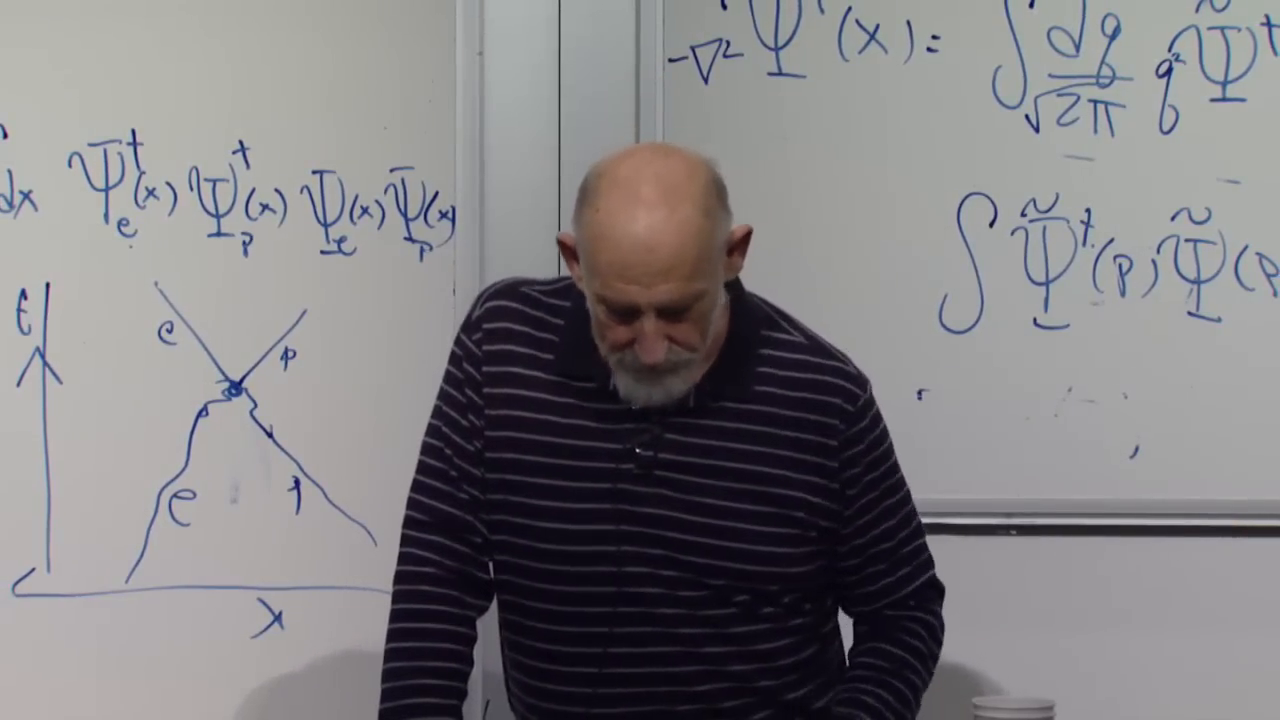
\includegraphics[width=0.94\linewidth]{lecture_09_frame_02.png}
\caption{Контактное взаимодействие на доске. Четыре локальных полевых оператора показаны над пространственно-временной схемой; точка встречи — единственное место, где действует идеализованное взаимодействие.}
\lectureframe{00:35:36}
\end{figure}

\begin{figure}[htbp]
\centering
\begin{tikzpicture}[x=1.2cm,y=1.0cm,>=Latex]
\draw[->] (-3.0,0) -- (3.0,0) node[right] {$x$};
\draw[->] (0,-0.2) -- (0,4.2) node[above] {$t$};
\coordinate (v) at (0,2.0);
\fill (v) circle (1.8pt);
\draw[thick,->] (-2.2,0.4) -- (v);
\draw[thick,->] (2.0,0.4) -- (v);
\draw[thick,->] (v) -- (-1.6,3.7);
\draw[thick,->] (v) -- (2.2,3.7);
\node[left] at (-1.65,0.7) {$e$};
\node[right] at (1.55,0.7) {$p$};
\node[left] at (-1.15,3.3) {$e$};
\node[right] at (1.65,3.3) {$p$};
\node[right] at (0.12,2.05) {$g$};
\end{tikzpicture}
\caption{Четкая реконструкция картины локального рассеяния. Вершина — это сокращенное обозначение оператора в уравнении~\eqref{eq:l9-contact}, а не классический закон столкновения.}
\end{figure}

Реальные электроны и протоны взаимодействуют на расстоянии через кулоновский потенциал. Контактная модель — лишь первый небольшой шаг: если бы эксперимент показал, что два вида частиц рассеиваются только при перекрытии, то в гамильтониан мы включили бы член вида ~\eqref{eq:l9-contact}.

\begin{classroomqa}
\lecturetimestamp{00:35:40}
\audiencequestion{Почему этот оператор рассеяния входит в гамильтониан, если энергия не меняется?}
\lecturerresponse{Гамильтониан — это и оператор энергии, и генератор, изменяющий состояние. Потенциальная энергия взаимодействия между двумя частицами порождает рассеяние при эволюции во времени. Сохранение полной энергии не означает, что состояние или отдельные импульсы частиц остаются неизменными.}
\end{classroomqa}

Это дает практическое правило. Сначала выясните из эксперимента, каким локальным процессам могут подвергаться частицы. Затем закодируйте эти процессы в операторе, который изменяет состояние. Произведения полей — не декоративная алгебра: множители с даггером и без него задают, какие виды частиц появляются и исчезают.

\section{Распад, обратный процесс и эрмитовость}

Предположим, что пузырьковая камера обнаруживает трек частицы вида \(A\), оканчивающийся в точке, из которой выходят треки \(B\) и \(C\). Локальный процесс имеет вид
\begin{equation}
A\longrightarrow B+C.
\end{equation}
Оператор, который его осуществляет, имеет вид
\begin{equation}
V=g\int dx\,
\psi_B^\dagger(x)\psi_C^\dagger(x)\psi_A(x).
\label{eq:l9-decay-half}
\end{equation}
Поле уничтожения уничтожает \(A\); два поля рождения создают \(B\) и \(C\) в одной и той же точке. Интегрирование с одинаковым весом по всем \(x\) выражает инвариантность относительно пространственных трансляций и сразу дает
\begin{equation}
p_A=p_B+p_C.
\end{equation}

Гамильтониан должен быть эрмитовым. Именно это делает \(e^{-itH}\) унитарным и обеспечивает сохранение полной вероятности. Выражение ~\eqref{eq:l9-decay-half} само по себе неэрмитово, поэтому мы должны добавить к нему эрмитово-сопряженный член:
\begin{equation}
H_{\mathrm{int}}
=\int dx\left[
g\,\psi_B^\dagger\psi_C^\dagger\psi_A
+g^*\,\psi_A^\dagger\psi_C\psi_B
\right](x).
\label{eq:l9-hermitian-vertex}
\end{equation}
Для вещественной константы связи \(g\) оба коэффициента совпадают. Эрмитово сопряжение не только заменяет поля с даггером на поля без него и наоборот, но и обращает порядок операторов. В этой игрушечной бозонной модели поля разных видов коммутируют, так что такое обращение не вызывает дополнительных осложнений.

Второй член осуществляет обратный процесс,
\begin{equation}
B+C\longrightarrow A.
\end{equation}
Следовательно, унитарный гамильтониан замкнутой системы, допускающий распад, также содержит амплитуду рекомбинации. Это не обещает, что оба направления реализуются для любого выбранного набора внешних импульсов; законы сохранения энергии и других величин могут сделать одно из направлений кинематически недоступным. Это означает, что и оператор, и его эрмитово-сопряженный член входят в динамику.

\begin{classroomqa}
\lecturetimestamp{00:42:48}
\audiencequestion{Может ли быть исключение из правила, что обратный процесс тоже разрешен?}
\lecturerresponse{Не на уровне эрмитова гамильтониана замкнутой системы: сопряженное взаимодействие обязательно. Конкретная обратная реакция все же может быть запрещена кинематикой или другим сохраняющимся квантовым числом, но сопряженный матричный элемент присутствует.}
\end{classroomqa}

Величина \(g\) — это константа связи. Если \(g\) мало, то встретившиеся частицы взаимодействуют лишь слабо; если оно велико, амплитуда перехода больше. Константы связи обычно являются параметрами, измеряемыми в экспериментах, хотя симметрии могут связывать несколько на вид различных констант связи.

Та же грамматика применима и к более сложным реакциям. В бета-распаде,
\begin{equation}
n\longrightarrow p+e^-+\bar\nu_e,
\end{equation}
схематический локальный член содержит четыре поля: одно уничтожает нейтрон, а три создают протон, электрон и электронное антинейтрино, вместе с эрмитово-сопряженным процессом. Этого достаточно, чтобы увидеть, как небольшой набор операторных мономов начинает задавать квантовую теорию поля.

\section{Почему важен квадрат гамильтониана}

В формуле для малого времени \eqref{eq:l9-short-update} сохранялся только первый порядок по \(\epsilon\). Полное разложение имеет вид
\begin{equation}
e^{-i\epsilon H}
=1-i\epsilon H-\frac{\epsilon^2}{2}H^2
+\frac{i\epsilon^3}{3!}H^3+\cdots.
\label{eq:l9-exponential}
\end{equation}
Во втором порядке гамильтониан действует дважды. В этом состоит алгебраическое происхождение первых изображений составных процессов.

Для вершины \(A\leftrightarrow B+C\) одно действие может объединить \(B+C\) в \(A\), а второе — снова превратить этот \(A\) в \(B+C\):
\begin{equation}
B+C\longrightarrow A\longrightarrow B+C.
\label{eq:l9-bc-scattering}
\end{equation}
В итоге получается вклад в амплитуду рассеяния \(B+C\to B+C\). Промежуточное \(A\) не является дополнительным наблюдаемым событием; оно обозначает состояние, по которому ведется суммирование между двумя действиями взаимодействия.

\begin{classroomqa}
\lecturetimestamp{00:49:54}
\audiencequestion{Должно ли поле \(C\) в записанном произведении второго порядка стоять с даггером?}
\lecturerresponse{Да, порядок операторов должен соответствовать указанной последовательности. Первая вершина уничтожает \(B\) и \(C\) и создает \(A\); вторая уничтожает \(A\) и вновь создает \(B\) и \(C\). Правильная расстановка даггеров восстанавливает именно эту интерпретацию.}
\end{classroomqa}

\begin{figure}[htbp]
\centering
\includegraphics[width=0.94\linewidth]{lecture_09_frame_05.png}
\caption{Две ориентации элементарной вершины \(A\leftrightarrow B+C\) на доске. Их расположение рядом — наглядная сокращенная запись процесса второго порядка из ~\eqref{eq:l9-bc-scattering}.}
\lectureframe{00:48:56}
\end{figure}

Теперь добавим спектаторную частицу \(B\). Одно действие позволяет \(A\) испустить \(C\) и превратиться в \(B\); последующее действие позволяет этому \(C\) соединиться с исходным \(B\) и образовать \(A\). Внешние частицы снова имеют виды \(A+B\), но их импульсы могут измениться. Мы описываем это как рассеяние \(A\) и \(B\) за счет обмена \(C\).

\begin{figure}[htbp]
\centering
\includegraphics[width=0.94\linewidth]{lecture_09_frame_06.png}
\caption{Построение обменного процесса на доске. Правая диаграмма соединяет две элементарные вершины внутренней линией \(C\), тогда как внешние частицы \(A\) и \(B\) рассеиваются.}
\lectureframe{00:51:22}
\end{figure}

\begin{figure}[htbp]
\centering
\begin{tikzpicture}[x=1.1cm,y=1cm,>=Latex]
\draw[->] (-3.7,-0.2) -- (-3.7,4.2) node[above] {$t$};
\coordinate (v1) at (-0.9,1.25);
\coordinate (v2) at (0.9,2.95);
\fill (v1) circle (1.7pt);
\fill (v2) circle (1.7pt);
\draw[thick,->] (-2.6,0.2) -- (v1) node[midway,below left] {$A$};
\draw[thick,->] (2.6,0.2) -- (v2) node[midway,below right] {$B$};
\draw[thick,->] (v1) -- (-2.4,4.0) node[midway,left] {$B$};
\draw[thick,->] (v2) -- (2.5,4.0) node[midway,right] {$A$};
\draw[thick,->,dashed] (v1) -- (v2) node[midway,above left] {$C$};
\node[below] at (0,-0.05) {$A+B\rightarrow A+B$};
\end{tikzpicture}
\caption{Аккуратная реконструкция обмена \(C\). Каждая точка вносит один множитель \(g\), так что этот член второго порядка пропорционален \(g^2\).}
\end{figure}

Каждая локальная точка взаимодействия называется вершиной. Каждая вершина вносит множитель своей константы связи, так что вклад с двумя вершинами несет \(g^2\), с тремя вершинами — \(g^3\) и так далее. Поэтому один-единственный член в гамильтониане связывает большое семейство реакций. Эта экономность — одна из причин, почему квантовая теория поля столь мощна: малое число локальных взаимодействий организует огромный массив данных о рассеянии.

\begin{classroomqa}
\lecturetimestamp{00:53:14}
\audiencequestion{Как называется процесс \(A\to B+C\to A\)?}
\lecturerresponse{Это вклад в собственную энергию. Наблюдаемое \(A\) — не просто голое одночастичное базисное состояние; у взаимодействующего состояния есть также амплитуда для близких компонент \(B+C\). Рассеяние на нем может выявить эту одетую структуру.}
\end{classroomqa}

Квантовая электродинамика дает знакомый пример. Локальная электрон--фотонная вершина может уничтожить электрон, вновь создать электрон и создать фотон. Во втором порядке электрон может испустить фотон и затем снова его поглотить. Заманчиво рассказывать об этом как о маленьком фильме, но в строгом смысле это член в пертурбативном разложении. Физический электрон — это одетое состояние с компонентами, содержащими фотон.

Оценка, приведенная на лекции, что эта компонента составляет ``около одного процента'', указывает на масштаб, задаваемый постоянной тонкой структуры, \(\alpha_{\mathrm{em}}\simeq 1/137\). Точная вероятность фоковской компоненты с фотоном зависит от энергетического разрешения и от того, как определено взаимодействующее состояние; это не универсальное свойство изолированного электрона на уровне одного процента. Надежное утверждение состоит в том, что взаимодействие изменяет измеримую структуру электрона.

\section{Что диаграмма говорит и чего она не говорит}

Диаграммы — это вычислительная сокращенная запись степеней гамильтониана взаимодействия. Они не являются надежными классическими историями, в которых частица определенно совершает одно событие, а затем другое. Попытка заглянуть внутрь и решить, какая промежуточная альтернатива ``действительно произошла'', меняет эксперимент и разрушает когерентную сумму, как и в обычной квантовой интерференции.

\begin{classroomqa}
\lecturetimestamp{00:56:52}
\audiencequestion{Сохраняются ли и энергия, и импульс в первой вершине?}
\lecturerresponse{В выполненной здесь гамильтоновой конструкции на равных временах пространственный интеграл сразу дает дельта-функцию по импульсу. Никакой интеграл по времени для этой отдельной вставки еще не дал дельта-функции по энергии. Полная амплитуда рассеяния, инвариантная относительно трансляций по времени, сохраняет полную энергию, тогда как промежуточные линии не обязаны удовлетворять соотношению на массовой поверхности, которому подчиняются наблюдаемые частицы. В ковариантном языке диаграмм четырехимпульс сохраняется в каждой вершине, но внутренние частицы могут быть вне массовой поверхности.}
\end{classroomqa}

Кажущееся отсутствие энергии в наивной картине вершины — еще одно предупреждение не отбрасывать энергию взаимодействия. Полный гамильтониан — это нечто большее, чем сумма энергий свободных частиц. Если возникает путаница, вернитесь к ~\eqref{eq:l9-exponential}: картинка обозначает член в разложении унитарной временной эволюции. Полная техника диаграмм Фейнмана систематически задает упорядочение по времени, пропагаторы, интегрирования и симметрийные множители, но базовая физика начинается уже здесь.

Развернутый вопрос слишком буквально трактует диаграмму, сравнивая испущенный фотон с электрическим полем, окружающим медленно движущийся электрон.

\begin{classroomqa}
\lecturetimestamp{00:58:26}
\audiencequestion{Создаётся ли электрическое поле электрона на расстоянии буквально испускаемыми фотонами? Как это согласуется с интерференцией и эффектом Ааронова--Бома?}
\lecturerresponse{Статическое, или индукционное, поле не является потоком реальных излучённых фотонов. Квантовая электродинамика описывает и излучение, и электромагнитное облачение электрона одним и тем же полем, но соответствующие квантовые состояния и кинематика различны. Для ультрарелятивистского электрона некоторые компоненты поля бывает полезно рассматривать как поток почти реальных фотонов; для медленного электрона модель буквальной траектории фотона неверна. Интерференция в опыте с двумя щелями и эффект Ааронова--Бома тоже являются неклассическими полевыми явлениями, но они не превращают эту диаграмму собственной энергии в механический фильм.}
\end{classroomqa}

\begin{classroomqa}
\lecturetimestamp{01:01:28}
\audiencequestion{Почему именно классическая модель диаграммы не работает?}
\lecturerresponse{Потому что вычисление когерентно суммирует амплитуды всех разрешённых промежуточных альтернатив. Опыт делает эти изображения интуитивно понятными, но их буквальное содержание никогда не выходит за пределы определяющего их операторного разложения. Это компактный способ вычислять \(H^2,H^3,\ldots\), а не запись наблюдаемых промежуточных событий.}
\end{classroomqa}

\begin{classroomqa}
\lecturetimestamp{01:03:04}
\audiencequestion{Может ли обычное кулоновское взаимодействие возникать как классический предел обмена фотонами?}
\lecturerresponse{Да. Вычисление соответствующей амплитуды, опосредованной фотоном, и переход к нерелятивистскому статическому пределу дают кулоновский потенциал. Этот вывод более техничен, чем настоящий операторный набросок, и его всё равно не следует понимать как буквальный прыжок фотона между двумя классическими частицами.}
\end{classroomqa}

\begin{classroomqa}
\lecturetimestamp{01:03:44}
\audiencequestion{Вычисляются ли константы связи из произведений полей?}
\lecturerresponse{Обычно их численные значения берутся из эксперимента. Симметрия может накладывать на них ограничения или связывать константы связи, которые иначе были бы независимыми. Когда такое соотношение предсказывает относительные интенсивности различных реакций и эксперимент это подтверждает, такое согласие особенно информативно.}
\end{classroomqa}

\begin{classroomqa}
\lecturetimestamp{01:04:48}
\audiencequestion{Какова роль случайной симметрии по сравнению с калибровочной симметрией?}
\lecturerresponse{Калибровочная симметрия напрямую ограничивает допустимую структуру и соотношения между константами связи. Случайная симметрия не задаётся на фундаментальном уровне, а возникает потому, что все разрешённые взаимодействия низшего порядка случайно ей удовлетворяют. Она всё же может иметь важные следствия, хотя её происхождение и устойчивость отличаются от таковых у калибровочной симметрии.}
\end{classroomqa}

На этом с нерелятивистской теорией поля пока достаточно. Мы обещали фермионы. Вместо того чтобы сразу перейти к их вторичному квантованию, мы сначала разберём релятивистское одночастичное уравнение, которому должны удовлетворять их полевые операторы.

\section{Почему для электрона необходима теория относительности}

Начнём с одного пространственного измерения. Это нереалистичное ограничение, но оно устраняет геометрическую сложность трёхмерного спина, сохраняя при этом существенную алгебру. Электрон настолько лёгок, что релятивистские эффекты важны даже в атомах. В водороде его характерная скорость имеет порядок
\begin{equation}
v\sim\alpha_{\mathrm{em}}c\approx 0.007c,
\end{equation}
то есть примерно 1 процент скорости света. Для внутренних электронов в тяжёлом атоме характерный масштаб становится \(v\sim Z\alpha_{\mathrm{em}}c\), так что релятивистские поправки могут быть существенными. Что бы ни стало решающим мотивом — историческое любопытство или точность в атомной физике, — релятивистское уравнение типа Schr\"odinger физически необходимо.

Обычная процедура квантования начинается с классического соотношения между энергией и импульсом. В нерелятивистском случае
\begin{equation}
E=\frac{p^2}{2m},
\end{equation}
а подстановки
\begin{equation}
E\mapsto i\partial_t,
\qquad
p\mapsto-i\partial_x
\end{equation}
дают
\begin{equation}
i\partial_t\varphi(x,t)
=-\frac{1}{2m}\partial_x^2\varphi(x,t).
\end{equation}

Вместо этого теория относительности даёт, при \(c=1\),
\begin{equation}
E^2=p^2+m^2.
\label{eq:l9-rel-dispersion}
\end{equation}

\begin{figure}[htbp]
\centering
\includegraphics[width=0.94\linewidth]{lecture_09_frame_07.png}
\caption{Переход на доске от \(E=p^2/2m\) к релятивистскому соотношению \(E^2=p^2+m^2\) при \(c=1\).}
\lectureframe{01:10:30}
\end{figure}

Применяя подстановки к квадратному соотношению, получаем
\begin{equation}
-\partial_t^2\varphi
=\left(-\partial_x^2+m^2\right)\varphi,
\label{eq:l9-klein-gordon}
\end{equation}
или, что эквивалентно,
\begin{equation}
\left(\partial_t^2-\partial_x^2+m^2\right)\varphi=0.
\end{equation}
Это уравнение Клейна--Гордона. Это вполне осмысленное релятивистское полевое уравнение, особенно для полей со спином 0. Но искомое уравнение для электрона должно быть первого порядка по времени,
\begin{equation}
i\partial_t\Psi=H\Psi,
\end{equation}
чтобы эволюцию порождал сам \(H\), а не только \(H^2\).

Можно было бы формально выбрать
\begin{equation}
H=\sqrt{-\partial_x^2+m^2}.
\end{equation}
Квадратный корень можно корректно определить в импульсном пространстве, где он действует умножением на \(\sqrt{p^2+m^2}\), но в координатном пространстве это нелокальный псевдодифференциальный оператор. Он технически осмыслен, но эстетически бесполезен для локального уравнения, которое мы ищем. Поэтому начнём сначала.

\section{Безмассовая волна, движущаяся вправо}

Сначала рассмотрим безмассовую частицу, движущуюся вправо. Для её положительных энергии и импульса имеем
\begin{equation}
E=p
\qquad (c=1).
\end{equation}
Квантование даёт
\begin{equation}
i\partial_t\psi=-i\partial_x\psi,
\end{equation}
или
\begin{equation}
(\partial_t+\partial_x)\psi=0.
\label{eq:l9-right-mover}
\end{equation}
Любое решение имеет вид
\begin{equation}
\psi(x,t)=f(x-t).
\end{equation}
Профиль не меняет формы и движется вправо со скоростью света.

Сразу возникают две трудности. Во-первых, если допустить, чтобы уравнение ~\eqref{eq:l9-right-mover} действовало на произвольные фурье-моды, то отрицательный импульс имеет энергию \(E=p<0\), так что гамильтониан не ограничен снизу. Ручное ограничение условием \(p>0\) сохранило бы только праводвижущиеся состояния и ещё не дало бы той теории электрона, которая нам нужна. Во-вторых, это уравнение — дорога с односторонним движением: в нём нет обычного электрона, движущегося влево. Сначала мы решим проблему левого и правого движения, а отрицательные энергии пока оставим как есть.

\section{Две компоненты и матрица альфа}

Введём две амплитуды,
\begin{equation}
\Psi(x,t)=
\begin{pmatrix}
\psi_1(x,t)\\[3pt]
\psi_2(x,t)
\end{pmatrix},
\end{equation}
где \(\psi_1\) соответствует движению вправо, а \(\psi_2\) — движению влево в безмассовом пределе:
\begin{align}
(\partial_t+\partial_x)\psi_1&=0,
&
(\partial_t-\partial_x)\psi_2&=0.
\end{align}
Квантовая механика также допускает их произвольные суперпозиции. Поэтому частица может иметь амплитуды для обоих направлений, а не нести классическую метку, выбранную раз и навсегда.

Эта дополнительная двузначная степень свободы алгебраически напоминает спин, но в одном измерении это не обычный угловой момент. Определим
\begin{equation}
\alpha=
\begin{pmatrix}
1&0\\
0&-1
\end{pmatrix}
=\sigma_3.
\label{eq:l9-alpha}
\end{equation}
Её собственный вектор с собственным значением \(+1\) выделяет праводвижущуюся компоненту, а с собственным значением \(-1\) — леводвижущуюся. В безмассовой теории гамильтониан просто равен
\begin{equation}
H=\alpha p,
\end{equation}
и оба уравнения объединяются в
\begin{equation}
i\partial_t\Psi=-i\alpha\partial_x\Psi.
\label{eq:l9-massless-dirac}
\end{equation}

\begin{classroomqa}
\lecturetimestamp{01:22:44}
\audiencequestion{Как называется диагональная матрица, различающая две компоненты?}
\lecturerresponse{Как матрица Паули это \(\sigma_3\), а не \(\sigma_1\). В обозначениях Дирака для данной конструкции мы называем её \(\alpha\). Её алгебра — это привычная алгебра Паули, хотя физическая метка здесь обозначает направление, а не спиновый угловой момент.}
\end{classroomqa}

\begin{classroomqa}
\lecturetimestamp{01:23:32}
\audiencequestion{Приобретает ли эта конструкция более геометрический смысл в трёх измерениях, где направление является вектором?}
\lecturerresponse{Да. Трёхмерная задача требует по одной матрице для каждого пространственного направления и приводит к более богатой спинорной структуре. Тем не менее одномерная модель точна в своих рамках и выделяет существенную лево-правую алгебру без этой дополнительной сложности.}
\end{classroomqa}

\begin{figure}[htbp]
\centering
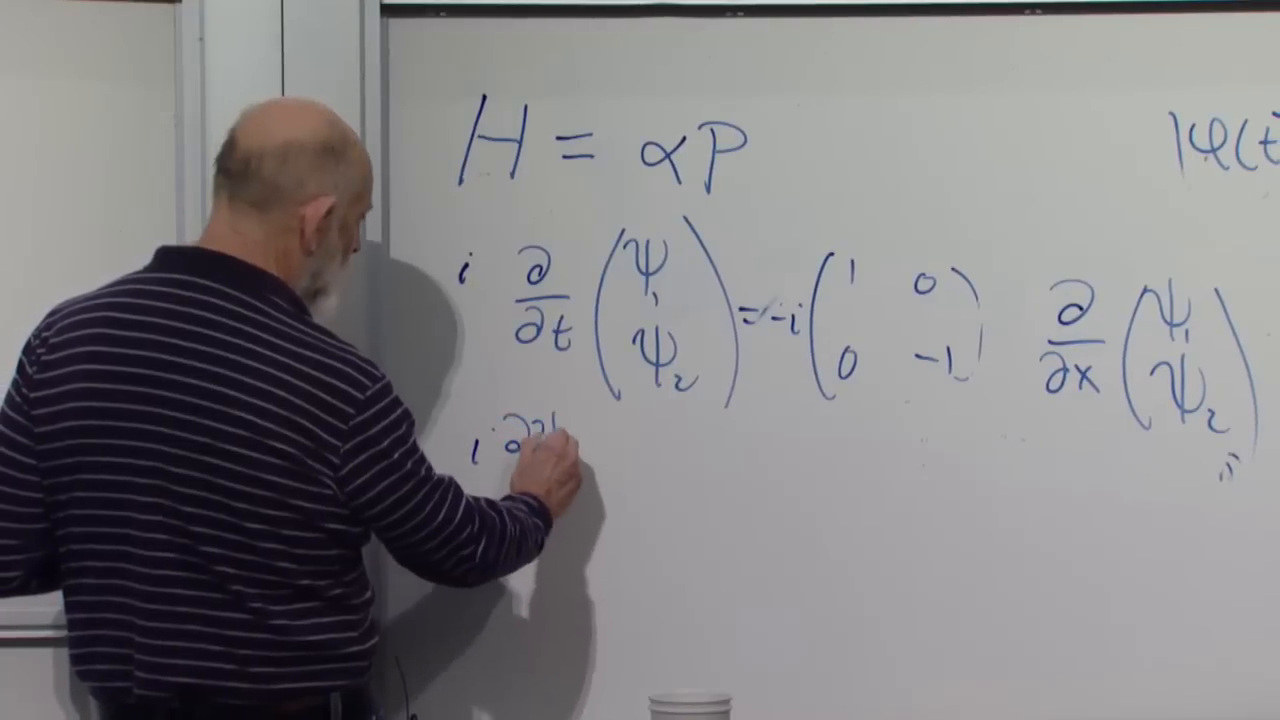
\includegraphics[width=0.94\linewidth]{lecture_09_frame_03.png}
\caption{Безмассовое двухкомпонентное уравнение на доске: \(H=\alpha P\), где диагональная матрица задаёт противоположные направления распространения для \(\psi_1\) и \(\psi_2\).}
\lectureframe{01:26:00}
\end{figure}

Проблема односторонности исчезла. Спектр с отрицательными энергиями остаётся, и мы обнаружили третий недостаток: обе компоненты по-прежнему безмассовы и распространяются со скоростью света. Следующий шаг должен ввести энергию покоя и связать эти направления.

\section{Добавление массы и открытие алгебры Дирака}

Добавим наиболее общий простой член, пропорциональный массе,
\begin{equation}
H=\alpha p+\beta m,
\label{eq:l9-dirac-hamiltonian}
\end{equation}
где \(\beta\) действует только на двухкомпонентный индекс. Это могла быть единичная матрица или какая-нибудь другая; предоставим выбор релятивистскому дисперсионному соотношению.

Поскольку \(H^2\) должно равняться \(p^2+m^2\), возведём в квадрат уравнение ~\eqref{eq:l9-dirac-hamiltonian}:
\begin{align}
H^2
&=(\alpha p+\beta m)^2\\
&=\alpha^2p^2+\beta^2m^2
+(\alpha\beta+\beta\alpha)pm.
\label{eq:l9-square-dirac}
\end{align}
Эти матрицы коммутируют с \(p\), потому что действуют во внутреннем двухкомпонентном пространстве, тогда как \(p\) действует на пространственную волновую функцию. Согласование с уравнением ~\eqref{eq:l9-rel-dispersion} требует
\begin{equation}
\alpha^2=\mathbb{1},
\qquad
\beta^2=\mathbb{1},
\qquad
\{\alpha,\beta\}
=\alpha\beta+\beta\alpha=0.
\label{eq:l9-dirac-algebra}
\end{equation}
Первое условие уже выполнено для \(\alpha=\sigma_3\). Любая другая матрица Паули антикоммутирует с ней и при возведении в квадрат даёт единичную матрицу. Выберем
\begin{equation}
\beta=
\begin{pmatrix}
0&1\\
1&0
\end{pmatrix}
=\sigma_1.
\label{eq:l9-beta}
\end{equation}
Выбор \(\sigma_1\) вместо \(\sigma_2\) — это вопрос соглашения о базисе; обе реализуют одну и ту же алгебру после унитарной замены базиса.

\begin{classroomqa}
\lecturetimestamp{01:33:00}
\audiencequestion{Неужели Дирак просто заметил, что матрицы Паули удовлетворяют этим алгебраическим условиям?}
\lecturerresponse{Исторически вывод сразу проводился в трёх измерениях и вводил матрицы, удовлетворяющие требуемым соотношениям. Как только условия записаны, алгебра Паули делает одномерное решение немедленным: достаточно выбрать две разные матрицы Паули.}
\end{classroomqa}

\begin{classroomqa}
\lecturetimestamp{01:34:24}
\audiencequestion{Является ли \(\beta\) релятивистским параметром скорости \(v/c\)?}
\lecturerresponse{Нет. Это матрица, действующая на компоненты спинора. Повторно используемая буква — всего лишь обозначение Дирака; она не имеет никакого отношения к кинематической величине \(v/c\).}
\end{classroomqa}

В трех пространственных измерениях матриц \(2\times2\) недостаточно для полного набора требуемых антикоммутирующих матриц. Это расширение отложено. В одном измерении уравнений~\eqref{eq:l9-alpha} и \eqref{eq:l9-beta} достаточно.

\section{Связанное одномерное уравнение Дирака}

Подстановка \(p=-i\partial_x\) дает одномерное уравнение Дирака в гамильтоновой форме:
\begin{equation}
i\partial_t\Psi
=\left(-i\alpha\partial_x+\beta m\right)\Psi.
\label{eq:l9-one-dimensional-dirac}
\end{equation}
Поскольку \(\alpha\) диагональна, ее член с производной оставляет две компоненты раздельными. Поскольку \(\beta\) внедиагональна, массовый член меняет их местами. Покомпонентно это записывается так:
\begin{align}
i\partial_t\psi_1
&=-i\partial_x\psi_1+m\psi_2,
\label{eq:l9-dirac-component-one}\\
i\partial_t\psi_2
&=+i\partial_x\psi_2+m\psi_1.
\label{eq:l9-dirac-component-two}
\end{align}

\begin{figure}[htbp]
\centering
\includegraphics[width=0.94\linewidth]{lecture_09_frame_08.png}
\caption{Связанные покомпонентные уравнения на доске. Противоположные знаки при производной кодируют движение вправо и влево; внедиагональный массовый член меняет местами \(\psi_1\) и \(\psi_2\).}
\lectureframe{01:37:44}
\end{figure}

Компоненты перестают эволюционировать независимо, как только \(m\ne0\). Возведение уравнения первого порядка в квадрат восстанавливает оператор Klein--Gordon для каждой компоненты,
\begin{equation}
\left(\partial_t^2-\partial_x^2+m^2\right)\psi_a=0,
\qquad a=1,2,
\end{equation}
а плоские волны удовлетворяют \(E^2=p^2+m^2\). Их групповая скорость равна
\begin{equation}
v_g=\frac{dE}{dp}=\frac{p}{E},
\end{equation}
модуль которой меньше единицы при ненулевой массе.

Связь между массой и смешением правого и левого секторов не случайна. Безмассовое праводвижущееся состояние остается праводвижущимся при любом собственном бусте Лоренца; никакой досветовой наблюдатель не может обогнать свет и обратить его направление. Массивную частицу можно привести в состояние покоя, а затем рассматривать из более быстрой системы отсчета, движущейся в том же направлении, где ее скорость кажется обращенной. Поэтому массивная релятивистская теория не может сохранять правый и левый секторы постоянно изолированными. Внедиагональный массовый член как раз и обеспечивает требуемую связь.

\begin{classroomqa}
\lecturetimestamp{01:40:01}
\audiencequestion{Является ли перестановка двух компонент хиральной осцилляцией?}
\lecturerresponse{В этом одномерном базисе \(\alpha\) различает два безмассовых хиральных направления. Массовый член внедиагонален и смешивает их, так что хиральность больше не сохраняется. В этом смысле массовый член является источником хиральной осцилляции.}
\end{classroomqa}

\begin{classroomqa}
\lecturetimestamp{01:40:46}
\audiencequestion{Почему уравнение фермиона должно быть квадратным корнем из уравнения бозона?}
\lecturerresponse{Так понимать это не следует. Дисперсионное соотношение \(E^2=p^2+m^2\) применимо к любой свободной релятивистской частице, независимо от статистики. Оператор Дирака просто дает матричную факторизацию оператора Klein--Gordon, но это алгебраическое соотношение не выводит фермионы из бозонов.}
\end{classroomqa}

\begin{classroomqa}
\lecturetimestamp{01:41:31}
\audiencequestion{Можно ли свести уравнение к простой скалярной факторизации на отдельные леводвижущиеся и праводвижущиеся множители?}
\lecturerresponse{Только в безмассовом пределе два хиральных уравнения расцепляются на независимые скалярные множители. При \(m\ne0\) полезна матричная факторизация: именно антикоммутирующие матрицы \(\alpha\) и \(\beta\) устраняют нежелательный перекрестный член.}
\end{classroomqa}

\begin{classroomqa}
\lecturetimestamp{01:42:04}
\audiencequestion{Составляют ли эти два связанных уравнения уже уравнение Дирака?}
\lecturerresponse{Да. Вместе они образуют уравнение Дирака в одном пространственном измерении; эквивалентно, оно записывается в компактной форме уравнения~\eqref{eq:l9-one-dimensional-dirac}. Более симметричную ковариантную запись можно получить, умножив на \(\beta\), но рассмотрение этой формы отложено.}
\end{classroomqa}

Две задачи намеренно оставлены незавершенными. Эта конструкция не устранила отрицательные энергии; она дала решения с отрицательной энергией в обоих секторах направлений движения, так что теперь эта проблема стала скорее более заметной, а не менее. Теория по-прежнему ограничена одним пространственным измерением. Следующие шаги — интерпретация решений с отрицательной энергией и расширение матричной алгебры до \(3+1\) измерений.

\chapter{Фермионы, матрицы Дирака и море Дирака}

Море Дирака — наша цель, но путь к нему тоже важен. Прежде чем столкнуться с отрицательной энергией в релятивистской теории электрона, нам понадобятся два элемента формализма. Сначала идет операторная алгебра, отличающая фермионы от бозонов. Затем — обзор одномерного уравнения Дирака, где любое расширение волновой функции можно проследить без геометрии трех пространственных измерений. Когда эти элементы будут на месте, трехмерное уравнение само потребует матричной структуры, а начальное обсуждение заполненных и пустых фермионных состояний вернется как ключ к позитронам.

Мы используем \(c=\hbar=1\). Заглавная \(P\) обозначает оператор импульса, строчная \(p\) — собственное значение импульса, а полужирные символы — их трехмерные версии.

\section{Обмен задается операторной алгеброй}

Рассмотрим две тождественные частицы, одну в \(x\) и другую в \(y\). Метки \(x\) и \(y\) обозначают полные положения; это не две декартовы координаты одной частицы. Действуя на вакуум двумя операторами рождения, получаем
\begin{equation}
\lvert x,y\rangle
=
\psi^\dagger(x)\psi^\dagger(y)\lvert0\rangle.
\label{eq:l10-two-particle-state}
\end{equation}

Для бозонов перестановка двух аргументов не меняет состояние:
\begin{equation}
\lvert x,y\rangle=\lvert y,x\rangle.
\end{equation}
Операторное утверждение, гарантирующее эту симметрию, имеет вид
\begin{equation}
\psi^\dagger(x)\psi^\dagger(y)
=
\psi^\dagger(y)\psi^\dagger(x).
\label{eq:l10-boson-exchange}
\end{equation}
Два бозонных оператора рождения коммутируют, поэтому мы можем менять их порядок, не изменяя создаваемое ими состояние.

Для фермионов перестановка меняет знак:
\begin{equation}
\lvert x,y\rangle=-\lvert y,x\rangle.
\label{eq:l10-fermion-state-exchange}
\end{equation}
Общий знак изолированного вектора состояния ненаблюдаем, но относительные знаки между альтернативами наблюдаемы, поэтому этот минус нужно последовательно сохранять. Из уравнения~\eqref{eq:l10-fermion-state-exchange} следует
\begin{equation}
\psi^\dagger(x)\psi^\dagger(y)
=
-\,\psi^\dagger(y)\psi^\dagger(x).
\label{eq:l10-fermion-operator-exchange}
\end{equation}

\begin{figure}[htbp]
\centering
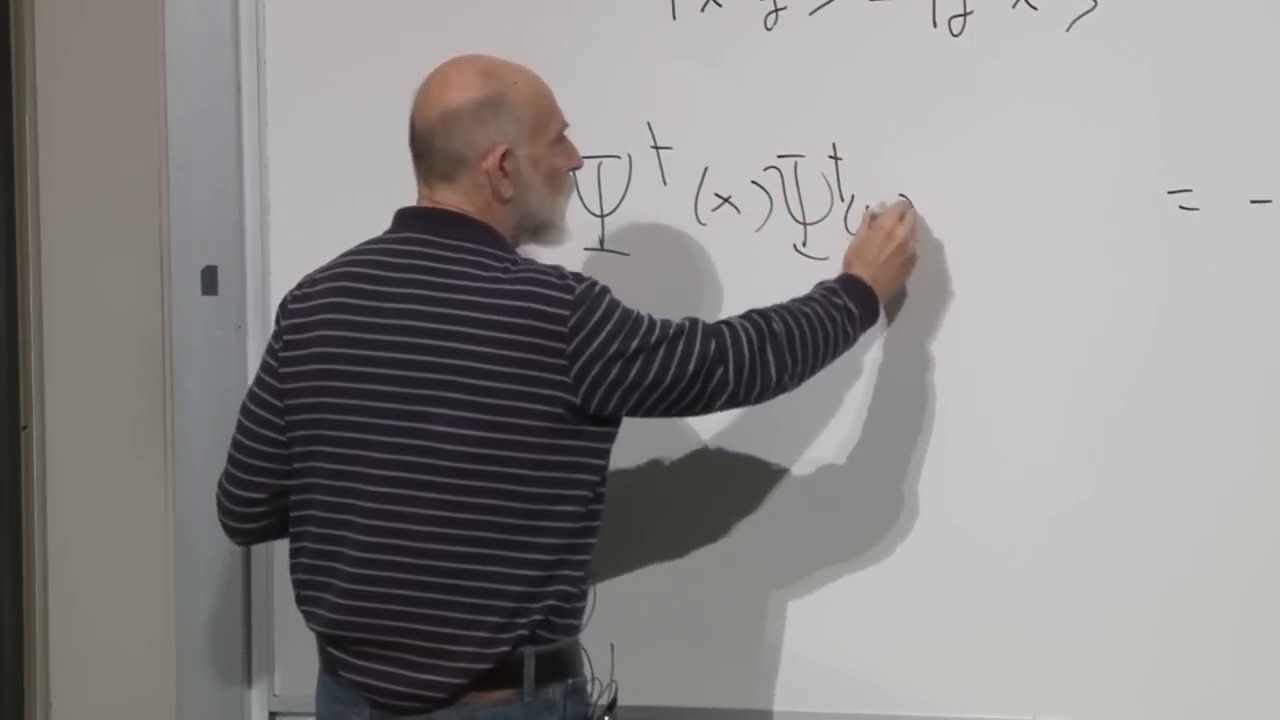
\includegraphics[width=0.94\linewidth]{lecture_10_figure_02.png}
\caption{Соотношение на доске, реализующее фермионный обмен. При перестановке операторов рождения знак двухчастичного состояния меняется на противоположный.}
\lectureframe{00:05:50}
\end{figure}

Для любых двух операторов \(A\) и \(B\) определим антикоммутатор как
\begin{equation}
\{A,B\}:=AB+BA.
\end{equation}
Поэтому правило обмена имеет вид
\begin{equation}
\{\psi^\dagger(x),\psi^\dagger(y)\}=0.
\label{eq:l10-creation-anticommutator}
\end{equation}
Соответствующая алгебра фермионного поля заменяет бозонные коммутаторы антикоммутаторами. Нужно различать два употребления этого термина: полевые операторы антикоммутируют в силу статистики Ферми, тогда как матрицы позднее будут антикоммутировать, чтобы устранить перекрестные члены в релятивистском дисперсионном соотношении.

Теперь положим \(y=x\) в уравнении~\eqref{eq:l10-creation-anticommutator}. Оба произведения становятся одинаковыми:
\begin{align}
0
&=\{\psi^\dagger(x),\psi^\dagger(x)\}\\
&=2\,\psi^\dagger(x)\psi^\dagger(x).
\end{align}
Следовательно,
\begin{equation}
\bigl(\psi^\dagger(x)\bigr)^2=0.
\label{eq:l10-exclusion}
\end{equation}
Попытка создать два тождественных фермиона в одном и том же одночастичном состоянии дает нулевой вектор. Это и есть принцип исключения в операторной форме.

\begin{figure}[htbp]
\centering
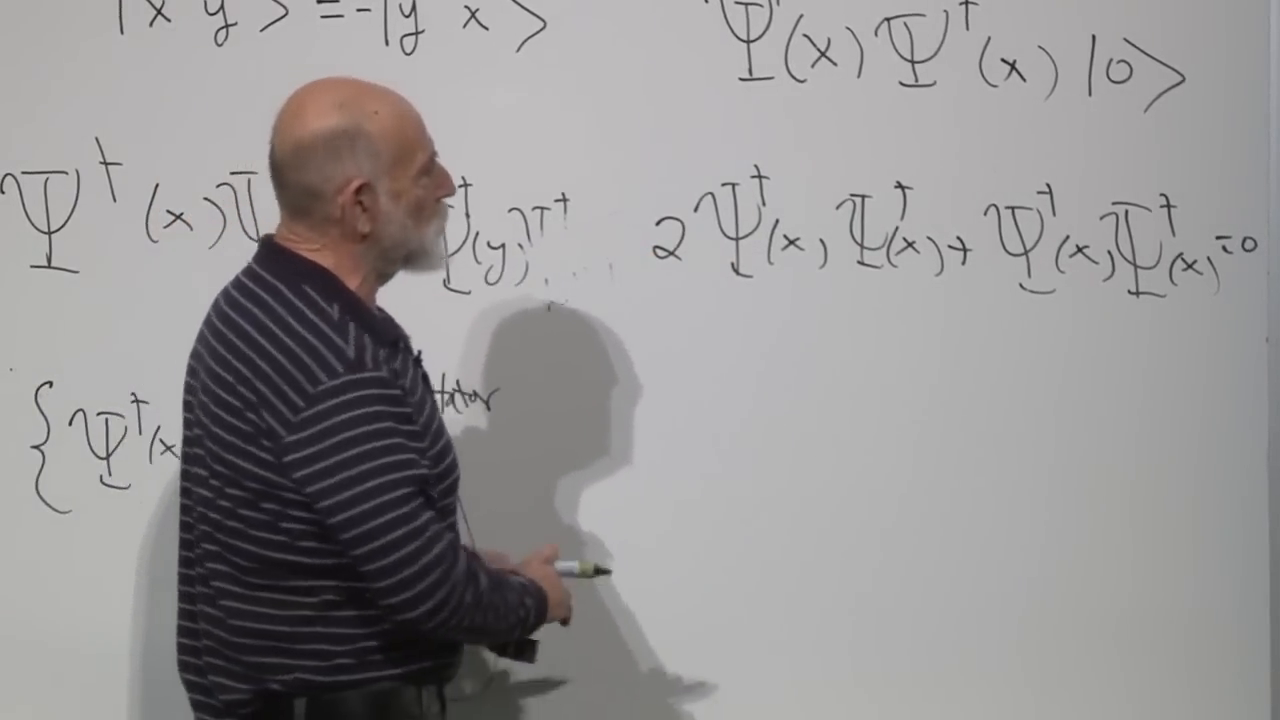
\includegraphics[width=0.94\linewidth]{lecture_10_figure_03.png}
\caption{Специализация на случай одинаковых состояний на доске. Произведение одного и того же оператора рождения появляется дважды и поэтому должно обращаться в нуль.}
\lectureframe{00:08:04}
\end{figure}

\begin{figure}[htbp]
\centering
\begin{adjustbox}{max width=\linewidth}
\begin{tikzpicture}[node distance=1.25cm,>=Latex]
\node[draw,rounded corners,align=center,inner sep=7pt] (a)
  {$\{\psi^\dagger(x),\psi^\dagger(x)\}=0$};
\node[draw,rounded corners,align=center,inner sep=7pt,right=of a] (b)
  {$2(\psi^\dagger(x))^2=0$};
\node[draw,rounded corners,align=center,inner sep=7pt,right=of b] (c)
  {$(\psi^\dagger(x))^2=0$};
\draw[->,thick] (a) -- (b);
\draw[->,thick] (b) -- (c);
\end{tikzpicture}
\end{adjustbox}
\caption{Вывод принципа исключения, восстановленный без частично стёртых промежуточных записей на доске.}
\end{figure}

\section{Почему заполненное и пустое симметричны для фермиона}

Есть и второе различие между бозонными и фермионными операторами, более тонкое, чем принцип исключения, и важное для дальнейшего. Для одной бозонной моды,
\begin{equation}
[a,a^\dagger]=1,
\qquad
n=0,1,2,\ldots.
\end{equation}
Перестановка \(a\) и \(a^\dagger\) меняет знак коммутатора. Даже если бы операторы просто назывались \(A\) и \(B\), алгебра сказала бы нам, какое упорядочение повышает число заполнения, а какое понижает его.

У бозонной лестницы заполнения тоже есть ориентация. Оператор уничтожения в конце концов доходит до \(\lvert0\rangle\) и дает нуль, тогда как оператор рождения может действовать неограниченно:
\begin{align}
a\lvert0\rangle&=0,\\
a^\dagger\lvert n\rangle&\propto\lvert n+1\rangle,
\qquad n=0,1,2,\ldots.
\end{align}
Если перевернуть эту лестницу вверх ногами, тот же спектр не получится. У нее есть низ, но нет верха.

Для одной фермионной моды,
\begin{equation}
\{a,a^\dagger\}=1,
\qquad
a^2=(a^\dagger)^2=0,
\qquad
n=0,1.
\label{eq:l10-fermion-mode}
\end{equation}
Оператор рождения переводит пустое состояние в заполненное, а затем останавливается:
\begin{equation}
a^\dagger\lvert0\rangle=\lvert1\rangle,
\qquad
a^\dagger\lvert1\rangle=0.
\end{equation}
Оператор уничтожения выполняет обратное:
\begin{equation}
a\lvert1\rangle=\lvert0\rangle,
\qquad
a\lvert0\rangle=0.
\end{equation}
Состояний только два, поэтому схема симметрична относительно замены заполненного на пустое и \(a\) на \(a^\dagger\). Физические смыслы операторов по-прежнему различны, но их алгебра уже не выделяет один как рождение, а другой как уничтожение. Эта формальная симметрия — зерно переинтерпретации частица–дырка.

\begin{classroomqa}
\lecturetimestamp{00:13:54}
\audiencequestion{Если \((a^\dagger)^2=0\), то это противоречие или отсюда следует, что \(a^\dagger=0\)?}
\lecturerresponse{Ни то ни другое. Ненулевой оператор может иметь обращающийся в нуль квадрат. Здесь \(a^\dagger\) переводит \(\lvert0\rangle\) в \(\lvert1\rangle\), но выше \(\lvert1\rangle\) допустимого состояния нет, поэтому двукратное применение дает нуль. То же рассуждение дает \(a^2=0\).}
\end{classroomqa}

Сохраним эту симметрию заполненного и пустого про запас. Когда электрон с отрицательной энергией удаляется, оператор уничтожения будет переобозначен как оператор рождения позитрона. Этот шаг — не произвольная смена обозначений; он использует в точности ту двухсостоянную фермионную алгебру, которая установлена здесь.

\section{Одномерная конструкция Дирака}

Теперь вернемся к одной частице в одном пространственном измерении. Простейшее релятивистское волновое уравнение первого порядка имеет вид
\begin{equation}
i\partial_t\psi=-\,i\partial_x\psi.
\label{eq:l10-right-mover}
\end{equation}
При \(P=-i\partial_x\) это
\begin{equation}
H=P.
\end{equation}
Для собственного состояния импульса имеем \(E=p\), а его групповая скорость равна
\begin{equation}
v_g=\frac{dE}{dp}=1.
\end{equation}
Положительный или отрицательный импульс, а значит, и положительная или отрицательная энергия, все равно дает волну, движущуюся вправо без изменения формы. Знак \(p\) меняет фазовый рисунок, а не направление распространения.

Массивная частица должна иметь возможность двигаться в любом направлении. Введем вторую компоненту, удовлетворяющую
\begin{equation}
H\psi_1=P\psi_1,
\qquad
H\psi_2=-P\psi_2.
\label{eq:l10-two-directions}
\end{equation}
Первая компонента движется вправо, вторая — влево. Объединим их в столбец,
\begin{equation}
\Psi=
\begin{pmatrix}
\psi_1\\
\psi_2
\end{pmatrix},
\end{equation}
и определим
\begin{equation}
\alpha=
\begin{pmatrix}
1&0\\
0&-1
\end{pmatrix}.
\end{equation}
Тогда оба уравнения принимают вид
\begin{equation}
H\Psi=\alpha P\Psi.
\label{eq:l10-massless-one-d}
\end{equation}
Цена включения обоих направлений — новая внутренняя степень свободы с двумя значениями.

Само по себе направление не порождает массу. Введем вторую матрицу,
\begin{equation}
\beta=
\begin{pmatrix}
0&1\\
1&0
\end{pmatrix},
\end{equation}
и попробуем
\begin{equation}
H=\alpha P+\beta m.
\label{eq:l10-massive-one-d}
\end{equation}
Эти матрицы удовлетворяют соотношениям
\begin{equation}
\alpha^2=\beta^2=\mathbb{1},
\qquad
\{\alpha,\beta\}=0.
\label{eq:l10-one-d-algebra}
\end{equation}
Возведение гамильтониана в квадрат дает
\begin{align}
H^2
&=(\alpha P+\beta m)^2\\
&=\alpha^2P^2+\beta^2m^2
  +(\alpha\beta+\beta\alpha)Pm\\
&=P^2+m^2.
\label{eq:l10-one-d-dispersion}
\end{align}
Антикоммутатор в уравнении~\eqref{eq:l10-one-d-algebra} устраняет нежелательный член, линейный и по \(P\), и по \(m\).

Недиагональная матрица \(\beta\) связывает две направленные компоненты. Полезно представлять массовый член как непрерывно смешивающий амплитуды, движущиеся вправо и влево. Эту картину не следует понимать буквально как частицу, отскакивающую туда-сюда по микроскопической траектории, но она передает, почему массивный волновой пакет может иметь среднюю скорость меньше скорости света и собственную систему отсчета, тогда как изолированная безмассовая хиральная компонента — нет.

\begin{classroomqa}
\lecturetimestamp{00:23:37}
\audiencequestion{Есть ли более глубокая физическая интерпретация введения обеих направленных компонент?}
\lecturerresponse{Есть, но яснее она проявится в трех измерениях. На этом этапе это просто две компоненты, необходимые для описания противоположных направлений распространения и для того, чтобы допустить недиагональную массовую связь. Их более поздняя интерпретация — лево- и праворукость, то есть хиральность.}
\end{classroomqa}

\section{Три измерения требуют матриц Паули}

В трех пространственных измерениях импульс является вектором. Поэтому гамильтониан, линейный по импульсу и скалярный относительно вращений, подсказывает другой вектор — теперь вектор, компонентами которого являются матрицы:
\begin{equation}
H=\boldsymbol{\alpha}\cdot\mathbf P
=\alpha_xP_x+\alpha_yP_y+\alpha_zP_z.
\label{eq:l10-three-d-ansatz}
\end{equation}

\begin{figure}[htbp]
\centering
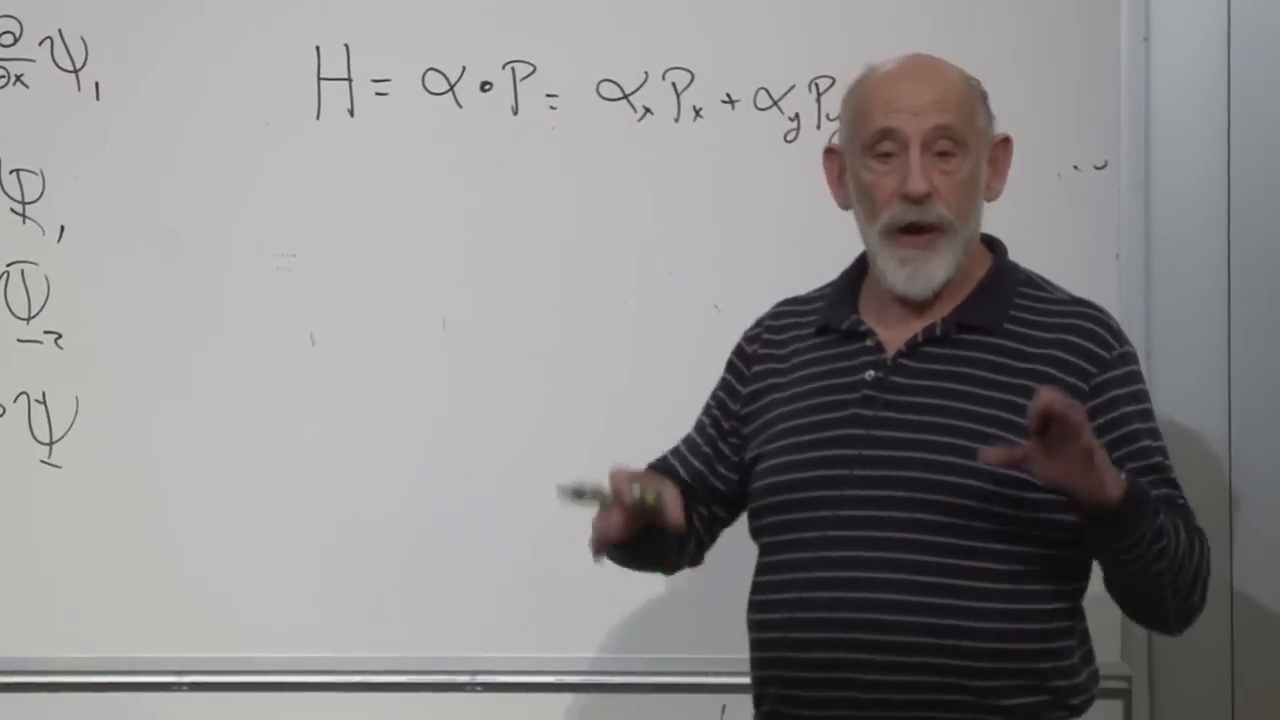
\includegraphics[width=0.94\linewidth]{lecture_10_figure_04.png}
\caption{Трехмерный безмассовый анзац \(H=\boldsymbol{\alpha}\cdot\mathbf P\) в тот момент, когда одна матрица становится вектором из трех матриц.}
\lectureframe{00:26:00}
\end{figure}

Снова начнем с безмассового случая. Мы требуем, чтобы
\begin{equation}
H^2=\mathbf P^2=P_x^2+P_y^2+P_z^2.
\end{equation}
Раскрывая квадрат уравнения~\eqref{eq:l10-three-d-ansatz},
\begin{align}
H^2
&=\alpha_x^2P_x^2+\alpha_y^2P_y^2\\
&\quad+\alpha_z^2P_z^2\\
&\quad+\{\alpha_x,\alpha_y\}P_xP_y\\
&\quad+\{\alpha_x,\alpha_z\}P_xP_z\\
&\quad+\{\alpha_y,\alpha_z\}P_yP_z.
\end{align}
Диагональные члены правильны, если
\begin{equation}
\alpha_x^2=\alpha_y^2=\alpha_z^2=\mathbb{1},
\end{equation}
а все перекрестные члены исчезают, если
\begin{equation}
\{\alpha_i,\alpha_j\}=0,
\qquad i\ne j.
\label{eq:l10-alpha-anticommutation}
\end{equation}

Три знакомые матрицы \(2\times2\) делают ровно это:
\begin{equation}
\sigma_x=
\begin{pmatrix}
0&1\\
1&0
\end{pmatrix},
\quad
\sigma_y=
\begin{pmatrix}
0&-i\\
i&0
\end{pmatrix},
\quad
\sigma_z=
\begin{pmatrix}
1&0\\
0&-1
\end{pmatrix}.
\label{eq:l10-pauli-matrices}
\end{equation}
Таким образом, одним из решений является
\begin{equation}
\alpha_i=\sigma_i,
\qquad
H=\boldsymbol{\sigma}\cdot\mathbf P.
\label{eq:l10-weyl-hamiltonian}
\end{equation}

\begin{figure}[htbp]
\centering
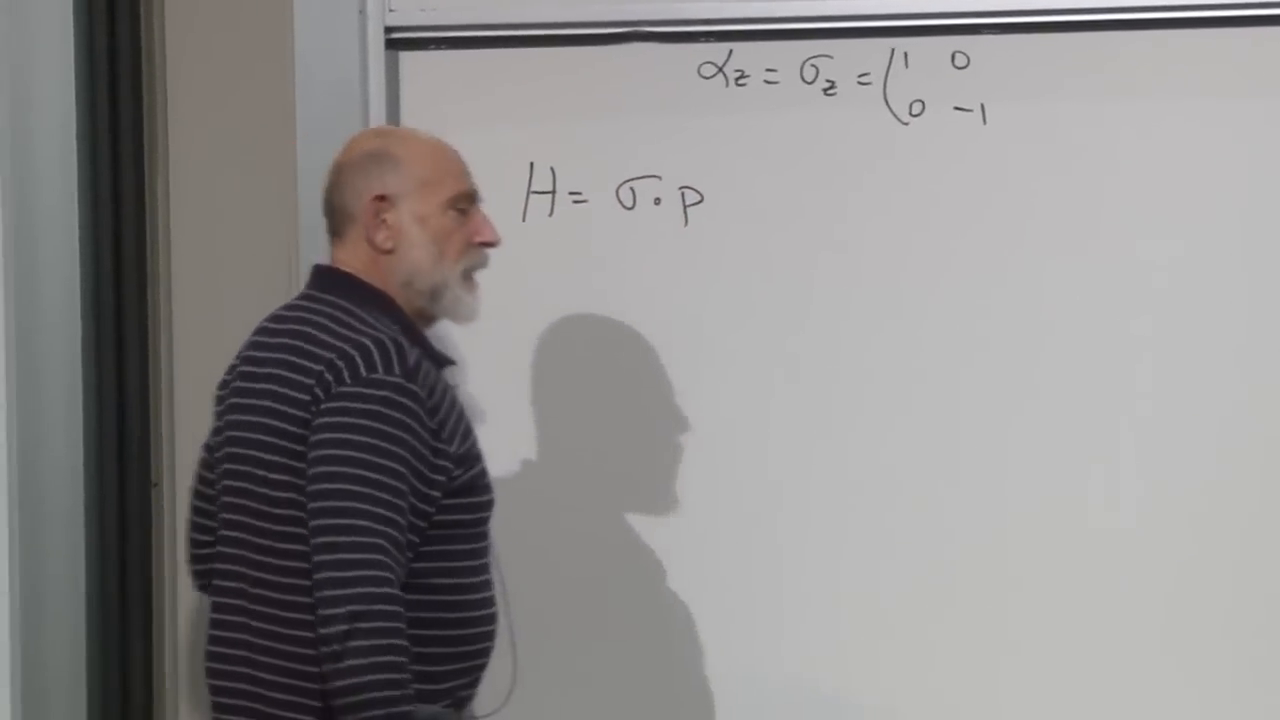
\includegraphics[width=0.94\linewidth]{lecture_10_figure_05.png}
\caption{Компактный безмассовый гамильтониан \(H=\boldsymbol{\sigma}\cdot\mathbf P\); над ним по-прежнему видна запись \(\alpha_z=\sigma_z\).}
\lectureframe{00:28:16}
\end{figure}

Для собственного состояния импульса,
\begin{equation}
\boldsymbol{\sigma}\cdot\mathbf p
=
|\mathbf p|\,\boldsymbol{\sigma}\cdot\widehat{\mathbf p}.
\end{equation}
Оператор \(\boldsymbol{\sigma}\cdot\widehat{\mathbf p}\) имеет собственные значения \(+1\) и \(-1\), так что
\begin{equation}
E=\pm|\mathbf p|.
\end{equation}
В этой двухкомпонентной теории положительной энергии соответствует степень свободы Паули, сонаправленная с импульсом, а отрицательной — направленная противоположно ему. Эта сонаправленность фиксирована; это не независимо выбираемое направление спина при фиксированном знаке энергии.

\begin{classroomqa}
\lecturetimestamp{00:30:10}
\audiencequestion{Спин «выпадает» из уравнения Дирака, или он был внесен потому, что уже известно, что у электрона есть магнитный момент?}
\lecturerresponse{Здесь «выпадает» означает «появляется как следствие», а не «исчезает». Исходным требованием был гамильтониан, линейный по импульсу, квадрат которого равен \(\mathbf P^2\). Обычные числа не могут удовлетворить требуемым алгебраическим соотношениям, а матрицы Паули могут. Поэтому их двухкомпонентная структура появляется вместе с самой линеаризацией. Это не доказывает, что каждая частица обязана иметь спин; это говорит о том, что частицы, описываемые уравнением дираковского типа, несут соответствующую спинорную степень свободы.}
\end{classroomqa}

Это один из центральных уроков данного построения. Матрицы — не декоративные метки, добавляемые после того, как найдено релятивистское уравнение. Их порождает попытка локально извлечь квадратный корень из релятивистского дисперсионного соотношения.

\section{Почему для массы нужны четыре компонента}

Попробуем повторить одномерное построение массы, не расширяя теорию \(2\times2\):
\begin{equation}
H=\boldsymbol{\sigma}\cdot\mathbf P+\beta m.
\label{eq:l10-failed-mass}
\end{equation}
Предположим, что \(\beta^2=\mathbb{1}\). Квадрат содержит требуемые члены \(\mathbf P^2+m^2\), но также содержит
\begin{equation}
m\sum_i\{\sigma_i,\beta\}P_i.
\end{equation}
Чтобы устранить этот член, матрица \(\beta\) должна была бы удовлетворять
\begin{equation}
\{\sigma_x,\beta\}
=
\{\sigma_y,\beta\}
=
\{\sigma_z,\beta\}
=0.
\label{eq:l10-impossible-beta}
\end{equation}
Ни одна матрица \(2\times2\) этому не удовлетворяет. Единичная матрица коммутирует со всеми тремя матрицами Паули, а всякая бесследовая матрица \(2\times2\) является линейной комбинацией матриц Паули. Любая такая комбинация не антикоммутирует с компонентой, параллельной ей. В алгебре \(2\times2\) нет четвёртой независимой матрицы требуемого вида.

Выход состоит в том, чтобы увеличить спинор. Четыре попарно антикоммутирующие матрицы, квадраты которых равны единичной матрице, впервые появляются в комплексном представлении \(4\times4\). Этот размер матриц выбирается не потому, что пространство-время четырёхмерно; это наименьшее матричное пространство, способное реализовать требуемую алгебру.

Существует много эквивалентных представлений. Унитарная замена спинорного базиса изменяет элементы всех матриц, не меняя ни одного физического предсказания. Существен лишь абстрактный набор соотношений
\begin{equation}
\{\alpha_i,\alpha_j\}=2\delta_{ij}\mathbb{1},
\qquad
\{\alpha_i,\beta\}=0,
\qquad
\beta^2=\mathbb{1}.
\label{eq:l10-dirac-algebra}
\end{equation}

\begin{classroomqa}
\lecturetimestamp{00:37:38}
\audiencequestion{Можно ли рассматривать \(\beta\) как временную компоненту \(\alpha_t\)?}
\lecturerresponse{Не напрямую. Три \(\alpha_i\) не образуют вместе с \(\beta\) четыре компоненты одного лоренцева вектора. В ковариантной записи вместо этого определяют \(\beta=\gamma^0\) и \(\alpha_i=\gamma^0\gamma^i\); четыре матрицы \(\gamma^\mu\) удовлетворяют пространственно-временной алгебре Клиффорда.}
\end{classroomqa}

Удобное блочное представление имеет вид
\begin{equation}
\alpha_i=
\begin{pmatrix}
\sigma_i&0\\
0&-\sigma_i
\end{pmatrix},
\qquad
\beta=
\begin{pmatrix}
0&I_2\\
I_2&0
\end{pmatrix}.
\label{eq:l10-block-representation}
\end{equation}
Матрицы Паули в диагональных блоках гарантируют, что различные \(\alpha_i\) антикоммутируют. Внедиагональные единичные блоки в \(\beta\) гарантируют, что \(\beta\) антикоммутирует с каждым \(\alpha_i\).

\begin{figure}[htbp]
\centering
\includegraphics[width=0.94\linewidth]{lecture_10_figure_06.png}
\caption{Блочное представление \(4\times4\), выписанное на доске. Верхние уравнения задают требуемые антикоммутаторы; полные матрицы набраны в уравнении~\eqref{eq:l10-block-representation}.}
\lectureframe{00:41:10}
\end{figure}

Массивный гамильтониан теперь имеет вид
\begin{equation}
H=\boldsymbol{\alpha}\cdot\mathbf P+\beta m
=
\begin{pmatrix}
\boldsymbol{\sigma}\cdot\mathbf P&mI_2\\
mI_2&-\boldsymbol{\sigma}\cdot\mathbf P
\end{pmatrix}.
\label{eq:l10-massive-dirac}
\end{equation}
Используя уравнение~\eqref{eq:l10-dirac-algebra},
\begin{equation}
H^2=\mathbf P^2+m^2.
\end{equation}
Следовательно, четырёхкомпонентная структура — не необязательное украшение. Это наименьшая структура, допускающая и трёхмерный импульс, и массовый член при сохранении уравнения первого порядка.

\section{Хиральность и смысл дополнительных компонент}

Какое физическое различие добавило это расширение? Начнём с безмассового верхнего блока,
\begin{equation}
H_R=\boldsymbol{\sigma}\cdot\mathbf P,
\end{equation}
и безмассового нижнего блока,
\begin{equation}
H_L=-\boldsymbol{\sigma}\cdot\mathbf P.
\end{equation}
Для состояний с положительной энергией у первого спин сонаправлен с импульсом, а у второго — антинаправлен. Это противоположные спиральности. В безмассовой теории спиральность инвариантна относительно собственных преобразований Лоренца, потому что ни один наблюдатель не может обогнать светоподобную частицу и обратить её импульс, оставив её спин неизменным. Поэтому два блока описывают противоположные хиральные секторы.

\begin{classroomqa}
\lecturetimestamp{00:41:28}
\audiencequestion{В одном измерении для введения массы требовалась дополнительная двоичная степень свободы. Какому физическому различию она соответствует в трёх измерениях?}
\lecturerresponse{Это хиральность спинора. Два блока \(2\times2\) задают противоположные соотношения между спином и импульсом. Один правохирален, другой левохирален. Теория \(4\times4\) содержит оба.}
\end{classroomqa}

Массовый член в уравнении~\eqref{eq:l10-massive-dirac} внедиагонален. Он переводит амплитуду верхнего блока в нижний и наоборот:
\begin{equation}
\beta m
\begin{pmatrix}
\Psi_R\\
\Psi_L
\end{pmatrix}
=
m
\begin{pmatrix}
\Psi_L\\
\Psi_R
\end{pmatrix}.
\end{equation}
Следовательно, масса представляет собой связь между противоположными хиральностями.

\begin{classroomqa}
\lecturetimestamp{00:43:58}
\audiencequestion{Может ли безмассовая частица изменить хиральность?}
\lecturerresponse{Не в свободном безмассовом гамильтониане, выписанном здесь. Два блока развязаны, так что состояние, начавшееся как правохиральное или левохиральное, таким и остаётся. Именно внедиагональный массовый член смешивает их при \(m\ne0\).}
\end{classroomqa}

Этот язык точен для блочного представления, но картину частицы, механически перескакивающей между двумя стрелками, не следует понимать слишком буквально. Физическое содержание состоит в матричной связи в волновом уравнении.

\begin{classroomqa}
\lecturetimestamp{00:44:50}
\audiencequestion{Содержатся ли эти матрицы уже в кватернионах?}
\lecturerresponse{Матрицы Паули тесно связаны с кватернионными единицами: матрицы \(-i\sigma_i\) возводятся в \(-\mathbb{1}\) и перемножаются по кватернионному правилу с точностью до соглашений об ориентации. Полные матрицы Дирака требуют большей алгебры Клиффорда, и для следующего рассуждения связь с кватернионами не нужна.}
\end{classroomqa}

\begin{classroomqa}
\lecturetimestamp{00:46:34}
\audiencequestion{Если спин — это момент импульса, есть ли здесь отдельный энергетический член, связанный с ним?}
\lecturerresponse{Нет, никакого независимого члена для свободной частицы не добавляется. Спинорная структура уже входит в кинетический гамильтониан через матрицы. Связь спина с внешним магнитным полем ввела бы дополнительные члены взаимодействия, но это другая задача.}
\end{classroomqa}

\section{Матрицы альфа — это скорость, а не спин}

У каждой \(\alpha_i\) есть два собственных значения \(+1\) и два собственных значения \(-1\). Различные компоненты не коммутируют, поэтому их нельзя все одновременно измерить точно. Чтобы определить, что представляет собой одна из компонент, воспользуемся уравнением Гейзенберга. Для оператора \(L\) без явной зависимости от времени,
\begin{equation}
\dot L=i[H,L].
\label{eq:l10-heisenberg}
\end{equation}
Здесь соглашение о знаке фиксируется эволюцией Schr\"odinger \(e^{-iHt}\).

Применим уравнение~\eqref{eq:l10-heisenberg} к оператору положения \(x\). Матрицы действуют на спинорные индексы и коммутируют с положением, тогда как только \(P_x\) не коммутирует с \(x\):
\begin{align}
\dot x
&=i[\boldsymbol{\alpha}\cdot\mathbf P+\beta m,x]\\
&=i\alpha_x[P_x,x]\\
&=\alpha_x,
\label{eq:l10-velocity}
\end{align}
поскольку \([P_x,x]=-i\). Следовательно, \(\alpha_x\) — это \(x\)-компонента оператора скорости; аналогично,
\begin{equation}
\dot{\mathbf x}=\boldsymbol{\alpha}.
\end{equation}

\begin{classroomqa}
\lecturetimestamp{00:51:50}
\audiencequestion{Неужели измерение компоненты скорости действительно даёт только \(+1\) или \(-1\)?}
\lecturerresponse{Да, для мгновенного оператора \(\alpha_i\) в единицах \(c=1\). Общее состояние не обязано быть собственным состоянием, поэтому его среднее значение может лежать где угодно между этими значениями. У гладко распространяющегося волнового пакета средняя скорость меньше световой, когда частица массивна.}
\end{classroomqa}

Скорость не сохраняется:
\begin{equation}
\dot\alpha_x=i[H,\alpha_x]\ne0.
\end{equation}
Слагаемые, содержащие \(\alpha_y\), \(\alpha_z\) и \(\beta\), не коммутируют с \(\alpha_x\). Поэтому состояние, содержащее компоненты как с положительной, так и с отрицательной энергией, даёт быстро осциллирующий вклад в положение. Это \emph{zitterbewegung}, буквально — дрожащее движение.

После усреднения по временам, большим по сравнению с быстрыми осцилляциями, ожидаемая релятивистская скорость равна
\begin{equation}
\overline{\mathbf v}=\frac{\mathbf p}{E},
\end{equation}
что для медленного электрона сводится к \(\mathbf p/m\).

\begin{classroomqa}
\lecturetimestamp{00:54:40}
\audiencequestion{Нарушает ли свободный электрон, дрожащий без внешней силы, закон Ньютона?}
\lecturerresponse{Нет. Трансляционная инвариантность сохраняет импульс, так что \(\dot{\mathbf P}=0\). Оператор скорости Дирака — не просто \(\mathbf P/m\), и его быстро осциллирующая часть может изменяться, тогда как импульс остаётся фиксированным. Усреднённое по времени движение подчиняется ожидаемому соотношению для свободной частицы.}
\end{classroomqa}

\begin{classroomqa}
\lecturetimestamp{00:55:22}
\audiencequestion{Всегда ли скорость равна \(c\)?}
\lecturerresponse{Мгновенное измерение одного \(\alpha_i\) имеет собственные значения \(\pm c\), но массивный волновой пакет, вообще говоря, является суперпозицией и имеет среднее значение меньше скорости света. Его средняя групповая скорость равна \(\mathbf p/E\).}
\end{classroomqa}

\begin{classroomqa}
\lecturetimestamp{00:55:30}
\audiencequestion{Можно ли понимать эти осцилляции так, будто масса изменяет скорость?}
\lecturerresponse{Нет. Масса — фиксированный параметр. Осцилляции возникают из-за некоммутирующих операторов скорости и гамильтониана, или, что эквивалентно, из-за интерференции между энергетическими секторами, а не из-за флуктуирующей массы.}
\end{classroomqa}

\begin{classroomqa}
\lecturetimestamp{00:56:22}
\audiencequestion{Может ли мгновенное измерение обнаружить скорость, направленную в одну сторону, даже если среднее движение направлено в другую?}
\lecturerresponse{Да. Оператор компоненты имеет два точных собственных значения, тогда как повторные или усреднённые по времени измерения восстанавливают более плавный дрейф.}
\end{classroomqa}

Слово спин тоже нужно употреблять осторожно. \(\alpha_i\) преобразуются как компоненты скорости, то есть обычного вектора. Подлинный оператор спина в этом представлении имеет вид
\begin{equation}
\mathbf S=\frac12\boldsymbol{\Sigma},
\qquad
\Sigma_i=
\begin{pmatrix}
\sigma_i&0\\
0&\sigma_i
\end{pmatrix}.
\label{eq:l10-spin-operator}
\end{equation}
Он отличается от \(\alpha_i\) знаком нижнего блока. Эти матрицы тесно связаны, но скорость и спин — не одна и та же наблюдаемая величина.

\section{Отрицательная энергия и вакуум с наименьшей энергией}

Проблема отрицательной энергии возникает уже до всего этого матричного аппарата. Вернёмся к одномерному праводвижущемуся состоянию,
\begin{equation}
H=P.
\end{equation}
Поскольку \(p\) пробегает всю вещественную ось, у \(E=p\) нет нижней границы.

Вакуум не может означать просто состояние без частиц. Он должен быть состоянием, из которого уже нельзя извлечь никакой дополнительной энергии. Если пустое состояние позволяет нам добавить частицу с отрицательной энергией, понизить энергию, добавить ещё одну и продолжать так бесконечно, то такое пустое состояние не является стабильным вакуумом.

Статистика Ферми исторически даёт выход. Поместим по одному электрону в каждое состояние с отрицательной энергией. Каждый добавленный электрон понижает полную энергию, но принцип запрета допускает только один электрон в каждом одночастичном состоянии. Когда все состояния с отрицательной энергией заполнены, никакой дополнительный электрон уже не может упасть в этот сектор. Дирак отождествил эту заполненную конфигурацию с вакуумом.

Та же конструкция не сработала бы для бозонов. Сколь угодно много бозонов может занимать одно состояние, так что бозонная мода с отрицательной энергией могла бы без ограничений поглощать частицы. Именно фермионное ограничение \(n=0,1\), введённое в начале лекции, и останавливает этот спуск.

\begin{figure}[htbp]
\centering
\includegraphics[width=0.94\linewidth]{lecture_10_figure_07.png}
\caption{Историческая картина моря Дирака на доске: лестница уровней отрицательной энергии, заполненных до разделяющей линии, а выше — состояния с положительной энергией.}
\lectureframe{01:02:45}
\end{figure}

\begin{figure}[htbp]
\centering
\begin{adjustbox}{max width=\linewidth}
\begin{tikzpicture}[x=1.05cm,y=0.72cm,>=Latex]
\draw[->] (0,-4.8) -- (0,4.8) node[above] {$E$};
\draw[thick] (-2.9,0) -- (3.2,0) node[right] {$E=0$};
\foreach \y in {-4,-3.3,...,-0.5} {
  \draw (-2.3,\y) -- (2.3,\y);
  \foreach \x in {-1.8,-1.2,...,1.8} {
    \fill[blue!65!black] (\x,\y) circle (1.6pt);
  }
}
\foreach \y in {0.8,1.6,...,4.0} {
  \draw (-2.3,\y) -- (2.3,\y);
}
\draw[red,very thick] (0.6,-2.6) circle (5pt);
\draw[red,->,very thick] (0.6,-2.35) .. controls (1.4,-0.4) and (1.2,1.6) .. (1.5,2.4);
\fill[red] (1.5,2.4) circle (2.5pt);
\node[right,red] at (0.85,-2.6) {hole};
\node[right,red] at (1.7,2.4) {$e^-$};
\node[left] at (-2.5,-2.2) {filled negative-energy states};
\end{tikzpicture}
\end{adjustbox}
\caption{Наглядная реконструкция возбуждения над заполненным морем: перевод одного электрона с отрицательной энергией оставляет дырку с положительной энергией.}
\end{figure}

Картина моря — это исторический язык для корректного переупорядочения операторов. Её буквальные бесконечные заряд и энергия не следует принимать за непосредственно наблюдаемые величины; современная переформулировка устранит необходимость представлять себе материальные электроны, заполняющие пространство.

\section{Дырка — это позитрон}

Когда все состояния с отрицательной энергией заняты, возможны два вида возбуждений. Можно добавить электрон с положительной энергией над морем. Или можно удалить один электрон с отрицательной энергией и оставить дырку.

Дырка имеет заряд, противоположный заряду отсутствующего электрона. Удаление заряда \(-e\) изменяет заряд на \(+e\). Она также имеет положительную энергию возбуждения. Если удалённый электрон имел \(E_-<0\), то энергия, измеренная относительно заполненного вакуума, изменяется на
\begin{equation}
E_{\mathrm{hole}}=-E_->0.
\end{equation}
Следовательно, дырка представляет собой возбуждение с положительной энергией и положительным зарядом: позитрон.

Фотон может перевести электрон из моря в состояние с положительной энергией. Относительно вакуума конечное состояние содержит электрон и позитрон. На диаграмме с временным упорядочением принято изображать поток электронного числа для электрона направленным вверх, а линию позитрона — со стрелкой в противоположную сторону. Эти стрелки отслеживают поток фермионного числа или заряда; это не маленькие классические векторы скорости.

\begin{classroomqa}
\lecturetimestamp{01:05:14}
\audiencequestion{Требует ли эта картина одинакового числа электронов и позитронов?}
\lecturerresponse{Не для произвольного состояния. Если начать с вакуума и создать нейтральную пару, получится по одному того и другого, но состояние уже может содержать избыток электронов или избыток позитронов. Сохранение заряда накладывает ограничения на реакции; оно не требует, чтобы в каждом допустимом состоянии их числа были равны.}
\end{classroomqa}

Дирак поначалу не знал, что дырка окажется частицей, тождественной электрону по массе и противоположной ему лишь по заряду и другим аддитивным квантовым числам. Уравнение и конструкция дырки привели к этому предсказанию ещё до того, как позитрон был включён в привычный каталог частиц.

\section{Одно фермионное поле содержит электроны и позитроны}

Оператор поля переводит историческую картину на язык современной алгебры. Пока опустим спинорные индексы, нормировочные множители и временную зависимость. Одномерное поле можно схематически разложить в виде
\begin{equation}
\psi(x)
\sim
\int_{-\infty}^{\infty}dp\,a(p)e^{ipx}.
\label{eq:l10-full-field-integral}
\end{equation}
Для праводвижущейся дисперсии \(E=p\) положительные значения \(p\) соответствуют положительной энергии, а отрицательные значения \(p\) — отрицательной. Разобьём интеграл:
\begin{equation}
\psi(x)
\sim
\int_0^\infty dp\,a(p)e^{ipx}
+
\int_{-\infty}^0 dp\,a(p)e^{ipx}.
\end{equation}
Во втором слагаемом положим \(p=-q\), где \(q>0\), и переинтерпретируем уничтожение заполненного электрона с отрицательной энергией как рождение позитрона:
\begin{equation}
b^\dagger(q):=a(-q).
\end{equation}
Тогда
\begin{equation}
\psi(x)
\sim
\int_0^\infty dp\,
\left[
a(p)e^{ipx}
+
b^\dagger(p)e^{-ipx}
\right].
\label{eq:l10-electron-positron-split}
\end{equation}
Точные знаки фаз плоских волн зависят от соглашения о пространстве-времени; инвариантное содержание состоит в том, что \(\psi\) содержит оператор уничтожения электрона и оператор рождения позитрона.

\begin{figure}[htbp]
\centering
\includegraphics[width=0.94\linewidth]{lecture_10_figure_08.png}
\caption{Интеграл по полю разделён на секторы положительной и отрицательной энергии. В нижней строке оператор электрона с отрицательной энергией переобозначается как оператор рождения позитрона.}
\lectureframe{01:11:35}
\end{figure}

Именно здесь оказывается полезной симметрия между занятым и пустым состояниями в ~\eqref{eq:l10-fermion-mode}. Для фермионов операторная алгебра допускает такое переобозначение без изменения её антикоммутационной структуры.

Схематически электромагнитное взаимодействие имеет вид
\begin{equation}
H_{\mathrm{int}}
\sim
\int dx\,\psi^\dagger(x)\psi(x)A(x),
\label{eq:l10-qed-schematic}
\end{equation}
где \(A\) обозначает фотонное поле. Поскольку каждое фермионное поле содержит электронную и позитронную части, один локальный оператор включает несколько каналов:
\begin{align}
e^-&\longrightarrow e^-+\gamma,\\
e^-+e^+&\longrightarrow\gamma,\\
\gamma&\longrightarrow e^-+e^+,
\end{align}
вместе с их обратными и скрещёнными процессами. Сохранение энергии и импульса решает, какой канал кинематически возможен в конкретной ситуации. Например, изолированный реальный фотон в вакууме не может создать пару без другого участника, который поглотил бы отдачу, хотя локальная вершина во взаимодействии присутствует.

\begin{figure}[htbp]
\centering
\includegraphics[width=0.94\linewidth]{lecture_10_figure_09.png}
\caption{На доске сопоставлены испускание фотона электроном, аннигиляция пары и схематическое взаимодействие \(\psi^\dagger\psi A\). Разные выборы из одних и тех же операторов поля порождают разные каналы.}
\lectureframe{01:13:30}
\end{figure}

Таким образом, одно компактное произведение полей охватывает множество на первый взгляд различных реакций. Позднее Фейнман дал систематические диаграммные правила для вычисления амплитуд, но значительная часть операторной структуры уже видна здесь.

\section{Современный язык вакуума и аналогия с морем Ферми}

\begin{classroomqa}
\lecturetimestamp{01:14:20}
\audiencequestion{Как современные физики описывают это, не рассматривая вакуум как буквальное море Дирака?}
\lecturerresponse{Они непосредственно выполняют операторную переинтерпретацию. Уничтожение электрона с отрицательной энергией переобозначается как рождение позитрона с положительной энергией, а вакуум определяется как состояние, уничтожаемое всеми операторами уничтожения электронов и позитронов. Получающаяся формулировка симметрична относительно частиц и античастиц и не нуждается ни в каком материальном море.}
\end{classroomqa}

Историческое море остаётся полезным, потому что его логика имеет близкий аналог в физике конденсированного состояния. В кристалле фиксированное число электронов заполняет самые низкие доступные одночастичные состояния вплоть до уровня Ферми. Заполненное основное состояние не пусто. Перевод одного электрона выше этого уровня оставляет под ним незанятое состояние. Относительно заполненного фона дырка несёт положительную энергию возбуждения и может вести себя как положительный носитель заряда.

Однако есть важные различия. Дырка в твёрдом теле живёт в среде, и её эффективная масса и зарядовый отклик зависят от зонной структуры. Позитрон — элементарная античастица в релятивистском квантовом поле. Тем не менее общая алгебра частица–дырка делает эту аналогию мощной.

\begin{classroomqa}
\lecturetimestamp{01:17:14}
\audiencequestion{Страдает ли теория Клейна--Гордона для бозонов тем же самым каскадным уходом в состояния с отрицательной энергией?}
\lecturerresponse{Нет. Правильно квантованное комплексное поле Клейна--Гордона строится из частиц и античастиц с положительной энергией без заполнения бозонного моря. Его уравнение второго порядка и каноническая структура отличаются от конструкции гамильтониана Дирака, поэтому исторический аргумент о фермионном море сюда без изменений не переносится.}
\end{classroomqa}

\begin{classroomqa}
\lecturetimestamp{01:17:30}
\audiencequestion{Откуда у бозонов берётся спин 1?}
\lecturerresponse{Не из линеаризации с помощью матриц Паули, использованной здесь. Поля со спином 1 имеют собственный закон преобразования Лоренца и собственные уравнения поля. Настоящий вывод объясняет спинорную структуру фермионов Дирака, а не все возможные спины частиц.}
\end{classroomqa}

\begin{classroomqa}
\lecturetimestamp{01:17:46}
\audiencequestion{Почему статистика Ферми была существенна для решения проблемы отрицательных энергий?}
\lecturerresponse{Потому что принцип запрета ограничивает каждое состояние одним электроном. Когда все состояния с отрицательной энергией заняты, ни один дальнейший электрон уже не может в них упасть. Для бозонной заселённости такого ограничения нет, так что буквальное море бозонов с отрицательной энергией всё равно не имело бы дна.}
\end{classroomqa}

\begin{classroomqa}
\lecturetimestamp{01:20:02}
\audiencequestion{Является ли различие между электроном и позитроном просто ещё одной двоичной степенью свободы, подобно заряду?}
\lecturerresponse{С точки зрения счёта состояний массивное поле Дирака имеет два спиновых состояния электрона и два спиновых состояния позитрона, так что две двоичные метки — полезная мнемоника. Но частица и античастица не являются независимо поворачиваемым внутренним кубитом одного электрона: каждый электрон имеет заряд \(-e\), каждый позитрон — \(+e\), и это различие возникает из секторов положительной и отрицательной частоты после квантования.}
\end{classroomqa}

Бесконечное море ставит напоследок ещё один вопрос.

\begin{classroomqa}
\lecturetimestamp{01:20:54}
\audiencequestion{Порождало бы бесконечное море Дирака бесконечную космологическую постоянную?}
\lecturerresponse{Здесь проявляется проблема энергии вакуума. Бозонные моды нулевых колебаний дают вклад \(+\tfrac12\hbar\omega\), тогда как фермионные моды дают вклад противоположного знака. Формальные компенсации возможны, когда спектры совпадают, но спектры электрона и фотона не совпадают, и ожидается огромный остаток. Без гравитации постоянный сдвиг гамильтониана можно вычесть, потому что имеют значение только разности энергий. При наличии гравитации абсолютная энергия вакуума гравитирует, так что такое вычитание становится физической проблемой, а не просто вопросом учёта.}
\end{classroomqa}

Последнее, к чему мы возвращаемся, — это смысл массы.

\begin{classroomqa}
\lecturetimestamp{01:22:56}
\audiencequestion{Можем ли мы сказать больше о том, как масса связывает левые и правые киральные компоненты?}
\lecturerresponse{Точное утверждение уже содержится в гамильтониане: внедиагональный член \(m\beta\) переводит один киральный блок в другой. Любая более механистическая картина такого микроскопического переключения необязательна и неизбежно неполна.}
\end{classroomqa}

\end{document}